%%%%%% Run at command line, run
%%%%%% xelatex grad-sample.tex 
%%%%%% for a few times to generate the output pdf file
\documentclass[12pt,oneside,openright,a4paper]{cpe-english-project}
\usepackage{algorithm}
\usepackage{algpseudocode}
\usepackage{polyglossia}
\usepackage{tabularx}
\usepackage{array}
\usepackage{float}
\usepackage{placeins}
\usepackage{hyperref}
\usepackage{listings}
\usepackage{color}
\setdefaultlanguage{english}
\setotherlanguage{thai}
\newfontfamily\thaifont[Script=Thai,Scale=1.23]{TH Sarabun New}
\defaultfontfeatures{Mapping=tex-text,Scale=1.0,LetterSpace=0.0}
\setmainfont[Scale=1.0,LetterSpace=0,WordSpace=1.0,FakeStretch=1.0]{Times New Roman}
\emergencystretch=10pt
%\XeTeXlinebreaklocale "th_TH"	
%\XeTeXlinebreakskip = 0pt plus 1pt
%\setmathfont(Digits)[Scale=1.0,LetterSpace=0,FakeStretch=1.0]{Times New Roman}
\lstloadlanguages{C,C++,csh,Java}
\definecolor{keywordcolor}{rgb}{0.1,0.3,0.6}
\definecolor{stringcolor}{rgb}{0.2,0.4,0.2}
\definecolor{commentcolor}{rgb}{0.4,0.4,0.4}
\definecolor{identifiercolor}{rgb}{0.1,0.1,0.1}
\definecolor{bgcolor}{rgb}{0.96,0.96,0.96}
\definecolor{framecolor}{rgb}{0.85,0.85,0.85}
\definecolor{captionbg}{rgb}{0.3,0.3,0.3}
\definecolor{gray}{gray}{0.5}

\lstset{
  language=csh,
  basicstyle=\footnotesize\ttfamily,
  numbers=left,
  numberstyle=\tiny\color{gray},
  numbersep=5pt,
  tabsize=2,
  extendedchars=true,
  breaklines=true,
  frame=b,
  stringstyle=\color{stringcolor}\ttfamily,
  showspaces=false,
  showtabs=false,
  xleftmargin=17pt,
  framexleftmargin=17pt,
  framexrightmargin=5pt,
  framexbottommargin=4pt,
  commentstyle=\color{commentcolor}\itshape,
  morecomment=[l]{//},
  morecomment=[s]{/*}{*/},
  showstringspaces=false,
  morekeywords={
    abstract, event, new, struct, as, explicit, null, switch,
    base, extern, object, this, bool, false, operator, throw,
    break, finally, out, true, byte, fixed, override, try,
    case, float, params, typeof, catch, for, private, uint,
    char, foreach, protected, ulong, checked, goto, public, unchecked,
    class, if, readonly, unsafe, const, implicit, ref, ushort,
    continue, in, return, using, decimal, int, sbyte, virtual,
    default, interface, sealed, volatile, delegate, internal,
    short, void, do, is, sizeof, while, double, lock, stackalloc,
    else, long, static, enum, namespace, string
  },
  keywordstyle=\color{keywordcolor}\bfseries,
  identifierstyle=\color{identifiercolor},
  backgroundcolor=\color{bgcolor},
  frame=single,
  rulecolor=\color{framecolor}
}


%%%%%%%%%%%%%%%%%%%%%%%%%%%%%%%%%%%%%%%%%%%%%%%%%%%%%%%%%%%%%%%%%%%
% Customize below to suit your needs 
% The ones that are optional can be left blank. 
%%%%%%%%%%%%%%%%%%%%%%%%%%%%%%%%%%%%%%%%%%%%%%%%%%%%%%%%%%%%%%%%%%%
% First line of title
\def\disstitleone{Adaptive Artificial Intelligence Agent for 2D Platformer Game Development}   
% Second line of title
\def\disstitletwo{}   
% Your first name and lastname
\def\dissauthor{Mr. Tanatanee Ponark}   % 1st member
%%% Put other group member names here ..
\def\dissauthortwo{Mr. Intouch Yusoh}   % 2nd member (optional)
\def\dissauthorthree{}   % 3rd member (optional)


% The degree that you're persuing..
\def\dissdegree{Bachelor of Engineering} % Name of the degree
\def\dissdegreeabrev{B.Eng} % Abbreviation of the degree
\def\dissyear{2024}                   % Year of submission
\def\thaidissyear{2567}               % Year of submission (B.E.)

%%%%%%%%%%%%%%%%%%%%%%%%%%%%%%%%%%%%%%%%%%%%
% Your project and independent study committee..
%%%%%%%%%%%%%%%%%%%%%%%%%%%%%%%%%%%%%%%%%%%%
\def\dissadvisor{Assoc.Prof. Natasha Dejdumrong, D.Tech.Sci.}  % Advisor
%%% Leave it empty if you have no Co-advisor
\def\disscoadvisor{}  % Co-advisor
%%% Leave it empty if you have no Co-advisor 2
\def\disscoadvisortwo{}  % Co-advisor 2 (if any)
\def\disscoadvisorthree{}  % Co-advisor 3 (You better be building space rocket or curing cancer at this point)
\def\disscommitteetwo{Asst.Prof. Nuttanart Muansuwan, Ph.D.}  % 3rd committee member (optional)
\def\disscommitteethree{Mr. Naveed Sultan}   % 4th committee member (optional) 
\def\disscommitteefour{Jaturon Harnsomburana, Ph.D.}    % 5th committee member (optional) 

\def\worktype{Project} %%  Project or Independent study
\def\disscredit{3}   %% 3 credits or 6 credits


\def\fieldofstudy{Computer Engineering} 
\def\department{Computer Engineering} 
\def\faculty{Engineering}

\def\thaifieldofstudy{วิศวกรรมคอมพิวเตอร์} 
\def\thaidepartment{วิศวกรรมคอมพิวเตอร์} 
\def\thaifaculty{วิศวกรรมศาสตร์}
 
\def\appendixnames{Appendix} %%% Appendices or Appendix

\def\thaiworktype{ปริญญานิพนธ์} %  Project or research project % 
\def\thaidisstitleone{ปัญญาประดิษฐ์ที่ปรับตัวได้สำหรับการพัฒนาเกม}
\def\thaidisstitletwo{}
\def\thaidissauthor{นายธนธานี โพธิ์นาค}
\def\thaidissauthortwo{นายอินทัช ยูโซะ} %Optional
\def\thaidissauthorthree{} %Optional

\def\thaidissadvisor{รศ.ดร.ณัฐชา เดชดำรง}
%% Leave this empty if you have no co-advisor
\def\thaidisscoadvisor{} %Optional
\def\thaidisscoadvisortwo{}  % Co-advisor 2 (if any)
\def\thaidisscoadvisorthree{} % Co-advisor 3 (You better be building space rocket or curing cancer at this point)
\def\thaidissdegree{วิศวกรรมศาสตรบัณฑิต}

% Change the line spacing here...
\linespread{1.15}

%%%%%%%%%%%%%%%%%%%%%%%%%%%%%%%%%%%%%%%%%%%%%%%%%%%%%%%%%%%%%%%%
% End of personal customization.  Do not modify from this part 
% to \begin{document} unless you know what you are doing...
%%%%%%%%%%%%%%%%%%%%%%%%%%%%%%%%%%%%%%%%%%%%%%%%%%%%%%%%%%%%%%%%


%%%%%%%%%%%% Dissertation style %%%%%%%%%%%
%\linespread{1.6} % Double-spaced  
%%\oddsidemargin    0.5in
%%\evensidemargin   0.5in
%%%%%%%%%%%%%%%%%%%%%%%%%%%%%%%%%%%%%%%%%%%
%\renewcommand{\subfigtopskip}{10pt}
%\renewcommand{\subfigbottomskip}{-5pt} 
%\renewcommand{\subfigcapskip}{-6pt} %vertical space between caption
%                                    %and figure.
%\renewcommand{\subfigcapmargin}{0pt}

\renewcommand{\topfraction}{0.85}
\renewcommand{\textfraction}{0.1}

\newtheorem{theorem}{Theorem}
\newtheorem{lemma}{Lemma}
\newtheorem{corollary}{Corollary}

\def\QED{\mbox{\rule[0pt]{1.5ex}{1.5ex}}}
\def\proof{\noindent\hspace{2em}{\itshape Proof: }}
\def\endproof{\hspace*{\fill}~\QED\par\endtrivlist\unskip}
%\newenvironment{proof}{{\sc Proof:}}{~\hfill \blacksquare}
%% The hyperref package redefines the \appendix. This one 
%% is from the dissertation.cls
%\def\appendix#1{\iffirstappendix \appendixcover \firstappendixfalse \fi \chapter{#1}}
%\renewcommand{\arraystretch}{0.8}
%%%%%%%%%%%%%%%%%%%%%%%%%%%%%%%%%%%%%%%%%%%%%%%%%%%%%%%%%%%%%%%%
%%%%%%%%%%%%%%%%%%%%%%%%%%%%%%%%%%%%%%%%%%%%%%%%%%%%%%%%%%%%%%%%


\begin{document}
\pdfstringdefDisableCommands{%
\let\MakeUppercase\relax
}
\begin{center}
  
\includegraphics[width=2.8cm]{logo02.jpg}
\end{center}
\vspace*{-1cm}

\maketitlepage
\makesignaturepage 

%%%%%%%%%%%%%%%%%%%%%%%%%%%%%%%%%%%%%%%%%%%%%%%%%%%%%%%%%%%%%%
%%%%%%%%%%%%%%%%%%%%%% English abstract %%%%%%%%%%%%%%%%%%%%%%%
%%%%%%%%%%%%%%%%%%%%%%%%%%%%%%%%%%%%%%%%%%%%%%%%%%%%%%%%%%%%%%
\abstract

In recent years, the application of artificial intelligence (AI) in game development has garnered significant attention, particularly in enhancing gameplay and automating testing processes. However, most existing AI systems are tailored for specific games or tasks, limiting their adaptability and reusability across different projects. This study proposes the development of an adaptive AI agent for 2D platformer games using reinforcement learning. The agent is trained within a Unity-based environment to learn essential player behaviors, such as movement, jumping, and obstacle avoidance. Leveraging the Proximal Policy Optimization (PPO) algorithm, the system is designed with modular components to promote flexibility, scalability, and ease of integration. By separating action execution from decision-making, the architecture facilitates the extension of the agent’s capabilities to support additional actions or mechanics. The trained AI model is packaged as a reusable Unity asset, intended for deployment in similar 2D games either as an intelligent NPC or an automated game tester. This approach aims to reduce development time and technical barriers for indie developers seeking to integrate intelligent behavior into their games. The results demonstrate the potential of reinforcement learning in constructing adaptable game agents and contribute toward making AI tools more accessible in the domain of game development.


\begin{flushleft}
\begin{tabular*}{\textwidth}{@{}lp{0.8\textwidth}}
\textbf{Keywords}: & Game Development / Artificial Intelligence / Enemy AI / Reusable Assets / Non-Player Characters / Adaptive AI / Reinforcement Learning / Procedural Learning / Game AI Training / AI Assets
\end{tabular*}
\end{flushleft}
\endabstract

%%%%%%%%%%%%%%%%%%%%%%%%%%%%%%%%%%%%%%%%%%%%%%%%%%%%%%%%%%%%%%
%%%%%%%%%% Thai abstract here %%%%%%%%%%%%%%%%%%%%%%%%%%%%%%%%%
%%%%%%%%%%%%%%%%%%%%%%%%%%%%%%%%%%%%%%%%%%%%%%%%%%%%%%%%%%%%%%
{
%\begin{thai}
\XeTeXlinebreaklocale "th_TH"	
\XeTeXlinebreakskip = 0pt plus 1pt
\thaifont
\thaiabstract

ในช่วงไม่กี่ปีที่ผ่านมา การประยุกต์ใช้ปัญญาประดิษฐ์ (AI) ในการพัฒนาเกมได้รับความสนใจอย่างมาก โดยเฉพาะในด้านการยกระดับประสบการณ์การเล่นเกมและการทดสอบระบบแบบอัตโนมัติ อย่างไรก็ตาม ระบบ AI ส่วนใหญ่ในปัจจุบันมักถูกออกแบบมาเพื่อใช้กับเกมหรือภารกิจเฉพาะเจาะจง ทำให้ขาดความยืดหยุ่นและไม่สามารถนำกลับมาใช้ซ้ำในโครงการอื่นได้อย่างมีประสิทธิภาพ งานวิจัยนี้นำเสนอการพัฒนาเอเจนต์ AI ที่สามารถปรับตัวได้สำหรับเกมแนวแพลตฟอร์มแบบ 2 มิติ โดยใช้เทคนิคการเรียนรู้เสริม (Reinforcement Learning) โดยเอเจนต์จะถูกฝึกในสภาพแวดล้อมที่พัฒนาบน Unity เพื่อเรียนรู้พฤติกรรมพื้นฐานของผู้เล่น เช่น การเคลื่อนที่ การกระโดด และการหลบหลีกสิ่งกีดขวาง ระบบนี้ใช้โครงข่ายนโยบายแบบ Proximal Policy Optimization (PPO) และออกแบบเชิงโมดูล เพื่อเพิ่มความยืดหยุ่น ขยายขอบเขตการใช้งาน และความสะดวกในการบูรณาการเข้ากับระบบอื่น โดยแยกกระบวนการตัดสินใจออกจากการดำเนินการ ทำให้สามารถต่อยอดเพื่อรองรับพฤติกรรมหรือกลไกเพิ่มเติมได้ง่ายขึ้น โมเดล AI ที่ผ่านการฝึกฝนแล้วจะถูกจัดทำเป็น Unity Asset ที่สามารถนำกลับมาใช้ซ้ำได้ในเกม 2 มิติที่มีลักษณะคล้ายกัน ไม่ว่าจะเป็นในบทบาทของตัวละคร NPC ที่มีความชาญฉลาด หรือเครื่องมือสำหรับการทดสอบเกมแบบอัตโนมัติ ซึ่งแนวทางนี้มีเป้าหมายเพื่อลดระยะเวลาในการพัฒนาและลดอุปสรรคทางเทคนิคสำหรับนักพัฒนาเกมอิสระที่ต้องการผสานพฤติกรรมอัจฉริยะเข้าสู่เกมของตน โดยผลการวิจัยแสดงให้เห็นถึงศักยภาพของการเรียนรู้เสริมในการสร้างเอเจนต์เกมที่สามารถปรับตัวได้ และสนับสนุนการเข้าถึงเครื่องมือ AI อย่างแพร่หลายในวงการพัฒนาเกม


\begin{flushleft}
\begin{tabular*}{\textwidth}{@{}lp{0.8\textwidth}}
 & \\

\textbf{คำสำคัญ}: & การพัฒนาเกม / ปัญญาประดิษฐ์ / ระบบศัตรูอัจฉริยะ / ทรัพยากรที่นำกลับมาใช้ได้ / ตัวละครที่ไม่ใช่ผู้เล่น / AI ที่ปรับตัวได้ / การเรียนรู้เสริม / การเรียนรู้แบบมีขั้นตอน / การฝึกสอน AI สำหรับเกม / ทรัพยากร AI
\end{tabular*}
\end{flushleft}
\endabstract
%\end{thai}
}

%%%%%%%%%%%%%%%%%%%%%%%%%%%%%%%%%%%%%%%%%%%%%%%%%%%%%%%%%%%%
%%%%%%%%%%%%%%%%%%%%%%% Acknowledgments %%%%%%%%%%%%%%%%%%%%
%%%%%%%%%%%%%%%%%%%%%%%%%%%%%%%%%%%%%%%%%%%%%%%%%%%%%%%%%%%%
\preface
\quad This research project, Adaptive Artificial Intelligence Agent in Game Development, was conducted as part of the academic curriculum of the Department of Computer Engineering, King Mongkut’s University of Technology Thonburi (KMUTT). The work presented in this report is the result of a collaborative effort between the authors, Mr. Intouch Yuso and Mr. Tanatanee Ponark, who have contributed equally to the research, design, and development of the system.\par

\quad We would first like to express our deepest gratitude to our advisor, \textbf {Assoc. Prof. Natasha Dejdumrong, D. Tech. Sci.,} for her exceptional guidance, continuous support, and insightful feedback throughout the entire project. Her expertise in artificial intelligence and game development served as a critical foundation for our research. Her mentorship not only helped shape the technical scope of the project but also encouraged us to pursue innovative and practical solutions.\par

\quad We would also like to extend our sincere thanks to our project committee members: \textbf {Asst. Prof. Nuttanart Muansuwan, Ph.D.,}, \textbf {Asst. Prof. Phond Phunchongharn, Ph.D.,} and \textbf {Dr. Jaturon Harnsomburana}, for their thoughtful evaluations, constructive criticisms, and valuable suggestions that greatly improved the overall quality of our work. Their diverse academic perspectives challenged us to think critically and approach the problem with greater depth and precision.\par

\quad We are grateful to the Department of Computer Engineering at KMUTT for providing the necessary infrastructure, software tools, and academic support that facilitated our experimentation and development processes. The collaborative environment and access to technical resources played a vital role in enabling us to execute our ideas effectively.\par

\quad Lastly, we would like to thank our families, friends, and classmates who offered their encouragement and moral support throughout the duration of the project. Their patience and motivation helped us stay focused and resilient, especially during difficult phases of development.To all who contributed to the success of this project directly or indirectly we offer our sincerest appreciation.\par

%%%%%%%%%%%%%%%%%%%%%%%%%%%%%%%%%%%%%%%%%%%%%%%%%%%%%%%%%%%%%
%%%%%%%%%%%%%%%% ToC, List of figures/tables %%%%%%%%%%%%%%%%
%%%%%%%%%%%%%%%%%%%%%%%%%%%%%%%%%%%%%%%%%%%%%%%%%%%%%%%%%%%%%
% The three commands below automatically generate the table 
% of content, list of tables and list of figures
\tableofcontents                    
\listoftables
\listoffigures                      

%%%%%%%%%%%%%%%%%%%%%%%%%%%%%%%%%%%%%%%%%%%%%%%%%%%%%%%%%%%%%%
%%%%%%%%%%%%%%%%%%%%% List of symbols page %%%%%%%%%%%%%%%%%%%
%%%%%%%%%%%%%%%%%%%%%%%%%%%%%%%%%%%%%%%%%%%%%%%%%%%%%%%%%%%%%%
% You have to add this manually..
\listofsymbols
\begin{flushleft}
\begin{tabular}{@{}p{0.07\textwidth}p{0.7\textwidth}p{0.1\textwidth}}
\textbf{SYMBOL}  & & \textbf{UNIT} \\[0.2cm]
$\alpha$ & Test variable\hfill & m$^2$ \\
$\lambda$ & Interarival rate\hfill &  jobs/second\\
$\mu$ & Service rate\hfill & jobs/second\\
\end{tabular}
\end{flushleft}
%%%%%%%%%%%%%%%%%%%%%%%%%%%%%%%%%%%%%%%%%%%%%%%%%%%%%%%%%%%%%%
%%%%%%%%%%%%%%%%%%%%% List of vocabs & terms %%%%%%%%%%%%%%%%%
%%%%%%%%%%%%%%%%%%%%%%%%%%%%%%%%%%%%%%%%%%%%%%%%%%%%%%%%%%%%%%
% You also have to add this manually..
\listofvocab
\begin{flushleft}
\begin{tabular}{@{}p{1in}@{=\extracolsep{0.5in}}p{0.73\textwidth}}
AI & Artificial Intelligence \\
NPC & Non Player Characters  \\
RL & Reinforcement Learning \\
\end{tabular}
\end{flushleft}

%\setlength{\parskip}{1.2mm}

%%%%%%%%%%%%%%%%%%%%%%%%%%%%%%%%%%%%%%%%%%%%%%%%%%%%%%%%%%%%%%%
%%%%%%%%%%%%%%%%%%%%%%%% Main body %%%%%%%%%%%%%%%%%%%%%%%%%%%%
%%%%%%%%%%%%%%%%%%%%%%%%%%%%%%%%%%%%%%%%%%%%%%%%%%%%%%%%%%%%%%%


\chapter{Introduction}

\section{Background}

Platformer games, characterized by side-scrolling environments, real-time control, and obstacle navigation, have remained a cornerstone of the video game industry. From early classics like Super Mario Bros. to modern indie titles such as Celeste and Hollow Knight, 2D platformers continue to thrive due to their accessible mechanics, expressive level design, and broad audience appeal. These games often serve as entry points for indie developers due to their design simplicity and well-established conventions.\par

A central component of platformer gameplay lies in the design of intelligent agents. Whether as playable characters or non-player characters (NPCs), these agents must exhibit responsive, believable behavior within dynamic environments. Traditionally, such behavior is implemented using finite state machines or behavior trees, rule-based systems that are straightforward to construct and maintain. However, these methods often produce rigid, predictable behavior that lacks adaptability in complex scenarios.\par

In contrast, reinforcement learning (RL), a subfield of machine learning, offers a more flexible and scalable approach to agent behavior. By learning through trial-and-error interaction with the environment, RL agents discover policies that maximize long-term cumulative rewards. This paradigm enables AI agents to adapt autonomously to changes in game conditions, mechanics, and objectives. RL has shown great potential in various domains such as robotics, autonomous navigation, and advanced gameplay systems.\par

Despite these advantages, the adoption of reinforcement learning in commercial game development remains limited. RL-based systems are typically confined to academic research or high-budget productions, primarily due to their steep learning curve, extensive training requirements, and lack of accessible tooling. Small studios and indie developers often lack the machine learning expertise, compute resources, and development time required to implement RL solutions effectively. Furthermore, most existing RL agents are purpose-built for specific games and environments, making them difficult to reuse or extend across projects.\par

This project aims to address these challenges by developing a modular, reusable AI framework tailored for 2D platformer games. The system is built within the Unity engine and leverages reinforcement learning to enable agents to perform essential platformer actions, such as walking, jumping, dashing, and obstacle avoidance, using a flexible, extensible architecture. The core design supports integration with external mechanics, custom environments, and retraining workflows\par

Although the focus is on 2D platformers, the framework is built with generalizability in mind. It aims to establish a foundation for developing scalable, adaptable AI agents that can be integrated into a range of game genres. By doing so, it addresses the gap between academic RL research and practical AI deployment in commercial game development, especially within the indie development space.\par

\section{Problem Statement}

Artificial intelligence is a critical component of modern video games, influencing enemy behavior, environmental interactivity, and automated testing. Yet for many small-scale and independent game studios, building intelligent, adaptive AI remains a significant hurdle. Traditional methods such as finite state machines and behavior trees dominate game AI implementation due to their ease of use and predictability. However, these approaches offer limited adaptability and scalability, often resulting in scripted, repetitive behaviors that require manual tuning and maintenance.\par

Reinforcement learning presents a compelling alternative by enabling agents to learn optimal behaviors through experience rather than predefined rules. However, RL implementations are typically developed for narrow use cases and tightly coupled to specific environments. This specialization limits their transferability, an agent trained for one game cannot easily be applied to another without extensive retraining or reengineering. This lack of generalization undermines RL's practical value for indie developers seeking flexible solutions that can adapt to different mechanics and level designs.\par

Furthermore, most existing RL toolkits and models are not designed with reusability in mind. They often lack modularity, documentation, or support for customization. Developers must invest considerable effort to integrate RL agents into existing projects, let alone extend them with new mechanics such as double-jumping or combat behavior.\par

This project seeks to address these limitations by delivering a reinforcement learning-based AI agent for 2D platformers that is not only pretrained but also modular, extensible, and easy to integrate. The agent learns to “solve” a platformer level by performing core gameplay actions, including traversal, object collection, and hazard avoidance, within a training environment constructed in Unity. Once trained, the model is exported as a Unity-compatible asset bundle that includes support components such as perception systems, action modules, and configuration files.\par

Importantly, the system is built to mimic the way human players generalize mechanical skills across games: a player who learns jumping and timing in one platformer can often apply that knowledge to another with similar mechanics. Likewise, this project aims to enable developers to reuse the pretrained agent across multiple games with comparable design principles, reducing training time, improving reliability, and supporting modular extension.\par

By lowering the barrier to entry for reinforcement learning in game development, this project provides a practical AI framework that supports not just a single application, but a family of games within a genre. It offers an efficient, scalable alternative to handcrafted AI systems for small teams working under constrained development resources.\par

\section{Objectives}
The primary goal of this project is to develop reusable, pretrained AI agents for 2D platformer games, delivered as a modular Unity asset that is easy to integrate, customize, and extend. The solution is designed to address the practical needs of indie developers by offering scalable AI functionality without requiring extensive machine learning expertise. The specific objectives are outlined as follows:
\subsection{Train Adaptive AI Agents for Platformer Mechanics}
\begin{itemize}
\item Train reinforcement learning (RL) agents capable of performing essential platformer behaviors, such as walking, jumping, dashing, and hazard avoidance, across varied level designs and gameplay scenarios.
\item Enable the AI agents to adapt to different environments and tasks without requiring full retraining.
\end{itemize}
\subsection{Develop a Modular and Reusable Unity Package}
\begin{itemize}
\item Package the trained AI models and support systems into a Unity-compatible asset that can be easily imported into other projects.
\item Design the architecture to be modular, allowing developers to add or remove functionality without modifying the core agent logic.
\end{itemize}
\subsection{Support Customization and Scalability}
\begin{itemize}
\item Implement an Action Module system that acts as a middleware layer, enabling developers to integrate their own control scripts with the pretrained agent through a standardized interface
\item Ensure the system is scalable to support additional mechanics such as double-jumping or ranged attacks by adding modular components.
\end{itemize}
\subsection{Establish a Generalizable AI Development Framework}
\begin{itemize}
\item Provide a structured framework that outlines best practices for training, evaluating, and extending AI agents in Unity-based projects.
\item Design the architecture for extensibility to future game genres beyond platformers.
\end{itemize}
\subsection{Deliver Comprehensive Documentation and Developer Resources}
\begin{itemize}
\item Include thorough documentation covering setup, customization workflows, and integration steps for different use cases.
\item Provide example scenes, tutorials, and retraining guides to support developers with varying levels of experience.
\end{itemize}

\section{Scope of Work}
This project is focused on the development of a reusable, pretrained AI framework for 2D platformer games using reinforcement learning techniques. The scope is defined by the genre, intended users, tools used, and practical boundaries that shape the project's direction.\par

\subsection{Project Focus}

The project is limited to the domain of 2D platformer games, chosen for their popularity, accessibility, and relevance to small and indie game development teams. The AI framework developed is intended to be integrated into Unity-based games, where agents must perform core platformer tasks such as movement, jumping, and hazard avoidance.

\subsection{Development Scope}

The scope includes the design of:
\begin{itemize}
\item A reinforcement learning-based AI agent capable of learning and performing platformer mechanics.
\item A modular system for integrating trained agents into different Unity projects with minimal adjustments.
\item A packaged Unity asset containing pretrained models, example environments, and documentation to support ease of use and further customization.
\end{itemize}

The project is designed with reusability, adaptability, and developer accessibility in mind, with a particular emphasis on supporting small game teams that may lack machine learning expertise.

\subsection{Boundaries and Limitations}

\begin{itemize}
\item The system is developed and tested solely for 2D platformer environments within Unity. Other genres or engines (e.g., 3D games, Unreal Engine) are not included in this scope.
\item Only the player agent is trained in this phase. While the system is extensible to enemy agents, adversarial training is reserved for future work.
\item The training process focuses on general platformer behavior rather than game-specific strategies, ensuring broad applicability at the expense of specialized behaviors.
\item The reinforcement learning approach is based on the Proximal Policy Optimization (PPO) algorithm provided by the Unity ML-Agents toolkit. Alternative algorithms are not explored in this work.
\end{itemize}

This scope provides a practical and clearly bounded framework for delivering a usable AI solution, while acknowledging limitations that define the context of the project's outcomes.

\section{Project Schedule}
The Gantt chart below (Figure \ref{fig:Gantt Chart}) illustrates the planned timeline for the project.
\begin{figure}[H]
\centering
\fbox{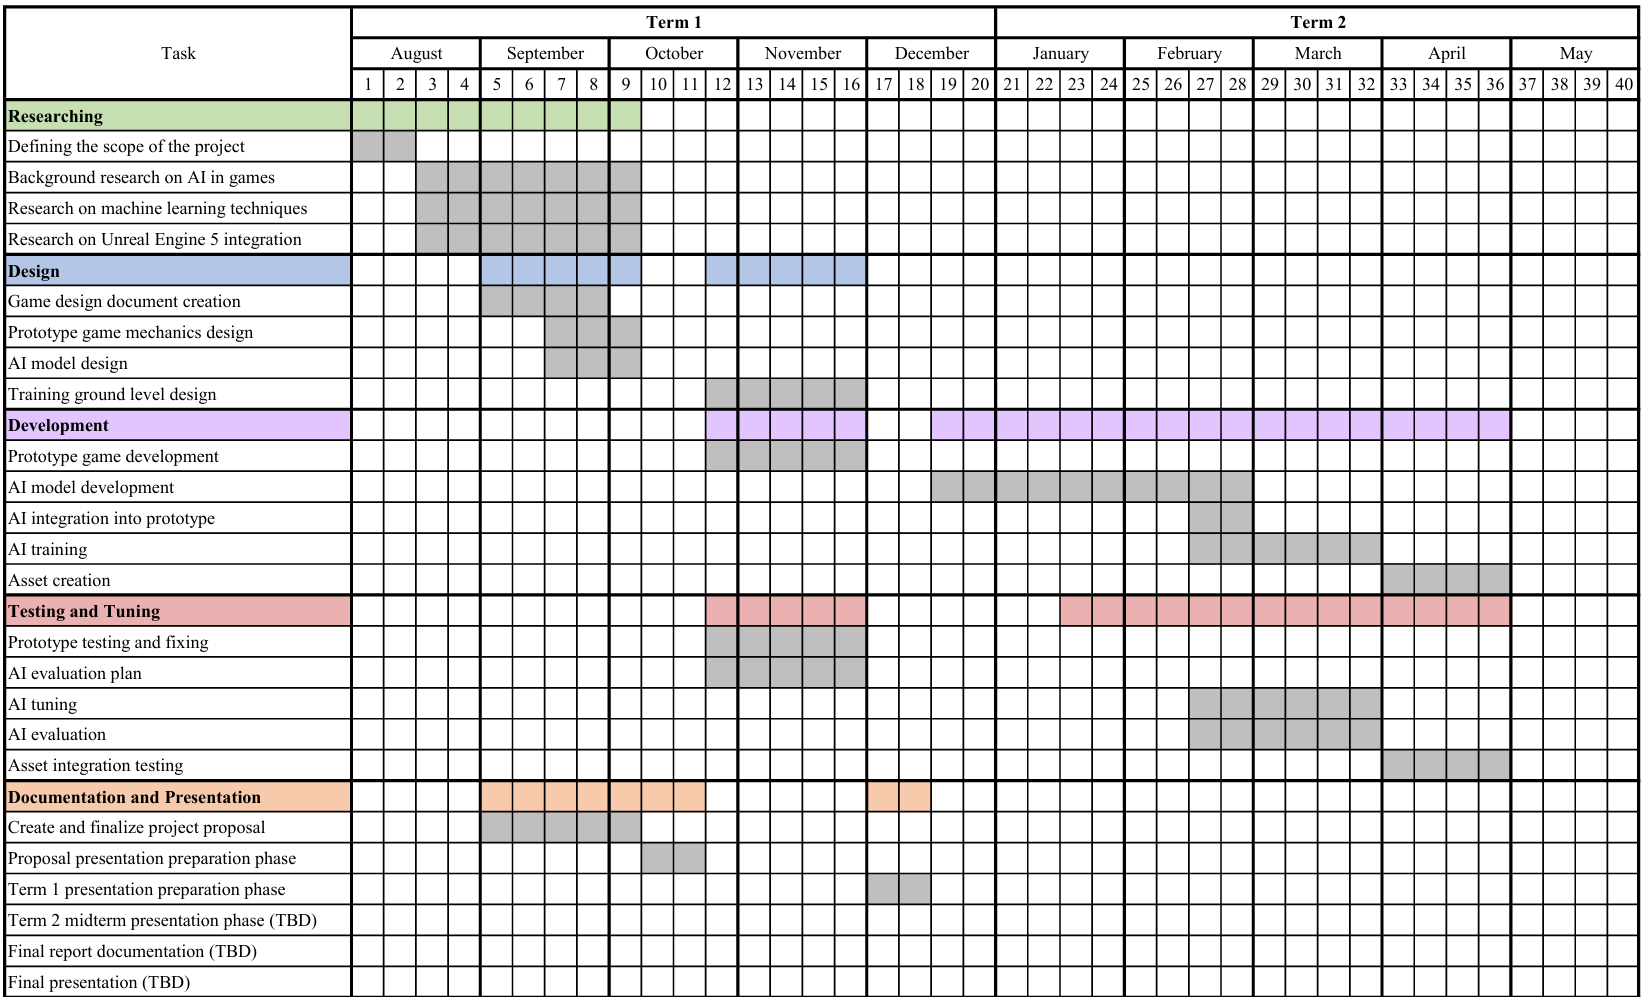
\includegraphics[width=15cm]{./Attachments/GanttChart.png}}
\caption{Gantt Chart}\label{fig:Gantt Chart}
\end{figure}
%%%%%%%%%%%%%%%%%%%%%%%%%%%%%%%%%%%%%%%%%%%%%%%%%%%%%%%%%%%%
%%%%%%%%%%%%%%  Literature Review %%%%%%%%%%%%%%%%%%%%%%%%%%
%%%%%%%%%%%%%%%%%%%%%%%%%%%%%%%%%%%%%%%%%%%%%%%%%%%%%%%%%%%%
\chapter{Background Theory and Related Work}
\section{Introduction}
This chapter presents the foundational theories and background knowledge required to understand the development of adaptive artificial intelligence (AI) agents within game environments. It covers essential machine learning concepts, particularly reinforcement learning, as well as the design principles relevant to interactive and dynamic gameplay. Additionally, the chapter introduces the development tools and frameworks used in this project, followed by a review of related research in the field. By examining existing AI methodologies and comparing them to the proposed system, this chapter highlights the technological context and motivation behind the project's design choices.

%This is how you add website url. -> \url{http://www.cpe.kmutt.ac.th}
%Explain theory, algorithms, protocols, or existing research works and tools related to your work.
%You can cite your references like this -> \cite{santi05b}  or multiplie cite like this -> \cite{bworld,hypersense}

\section{Theories and Core Concepts}
\subsection{Game Development}
Game development is a multidisciplinary process involving design, art, programming, and testing to create interactive digital experiences. This project focuses on 2D platformer games, a genre characterized by structured level design, real-time movement, and timing-based mechanics. Understanding how games are developed provides essential context for designing AI agents capable of functioning effectively in such environments.
\subsubsection{Game Development Lifecycle}
The process of developing a game typically consists of several phases, each building upon the previous:
\begin{itemize}
\item  \textbf{Pre-production:} This phase involves defining the game’s concept, genre, mechanics, art style, and development scope. It also includes creating design documentation and planning technical requirements.
\item  \textbf{Production:} The core development phase where game assets and systems are built. This includes character controllers, UI, level design, animations, physics, and audio integration.
\item  \textbf{Testing:} Debugging, performance testing, and gameplay balancing. AI behavior, especially if it is not deterministic, must be evaluated for reliability and consistency across different playthroughs.
\item  \textbf{Post-production:} Final refinements, bug fixes, performance optimizations, and user feedback integration. This stage also includes publishing, updates, and maintenance.
\end{itemize}
Game development often involves teams of varying sizes, from large studios with specialized departments to small indie teams handling multiple roles.
\subsubsection{Game Design}
Game design defines the systems and elements that shape a player's experience. Core areas include:
\begin{itemize}
\item  \textbf{Game Mechanics:}
The rules and interactions that define gameplay, movement, physics, progression, scoring, and objectives.
\item  \textbf{Narrative Design:}
Story elements that guide player engagement, from minimalistic setups to expansive, character-driven narratives.
\item  \textbf{Level Design:}
Crafting environments that balance pacing, challenge, and progression. Good level design introduces new elements incrementally and encourages exploration.
\item  \textbf{Assets:}
Game assets refer to the components used to build the visual, auditory, and interactive elements of a game. These include:
\begin{itemize}
\item  \textbf{Visual Assets:} Textures, 3D models, 2D sprites, animations, and visual effects that define the game's appearance.
\item  \textbf{Audio Assets:} Sound effects, background music, and character voices that create the auditory experience.
\item  \textbf{Code Assets:} Scripts and algorithms that govern game mechanics, AI behavior, and interactive elements.
\item  \textbf{UI Assets:} Menus, HUDs, buttons, feedback indicators, and other user interface components.
\end{itemize}
Assets are the building blocks of any game, providing the necessary materials to bring concepts to life. Their quality and integration play a significant role in defining the overall aesthetic and functionality of the game.
\item  \textbf{User Interface (UI) and User Experience (UX):}
The design of menus, HUDs (heads-up displays), and the interaction flow. A clean and intuitive UI is critical for keeping players immersed in the game.
\end{itemize}
\subsubsection{Game Design in 2D Platformers}
2D platformers are structured around character movement through levels composed of platforms, hazards, collectibles, and enemies. These games typically emphasize responsive controls, spatial awareness, timing, and feedback. Their mechanical clarity and visual simplicity make them ideal candidates for applying reinforcement learning techniques. Because platformers focus heavily on movement, navigation, and interaction with environmental objects, they provide a natural environment for testing AI performance in real-time gameplay contexts.\par
This genre is particularly relevant for this project because it is often chosen by indie developers due to its approachable development scope and strong potential for innovation. Solving AI challenges in this context can yield reusable and broadly applicable solutions.\par
\subsubsection{Game Teseting and Automation}
Game testing is critical to ensuring gameplay functionality, balance, and quality. It involves systematic evaluation of mechanics, interactions, and edge cases. Testing also plays a central role in identifying bugs, optimizing performance, and assessing the effectiveness of AI systems.\par
Traditionally, game testing is performed manually by QA testers or designers. This method is time-consuming and may not scale well with game complexity, especially for games with nonlinear progression, emergent behaviors, or multiple difficulty levels.\par
Automated testing tools have become increasingly useful, particularly for repeated simulation of gameplay scenarios. AI agents and scripted bots can be used to simulate playthroughs, identify unbalanced mechanics, and detect hard-to-find bugs. These agents also enable consistent data collection, such as completion time, failure points, or action frequencies, which supports more informed design decisions.\par
In recent years, machine learning has opened new possibilities for game testing. Reinforcement learning agents, for instance, can test levels by interacting adaptively with the environment, providing insight into player-like behavior. These methods are particularly valuable in open-ended or highly interactive games where traditional scripting approaches may fall short.\par
\subsubsection{Challenges Faced by Developers}
Game development, especially in small studios or solo efforts, presents several constraints:
\begin{itemize}
\item \textbf{Resource Limitations:} Small teams often lack access to advanced hardware, dedicated AI engineers, or large-scale testing capabilities.
\item \textbf{Complexity of Design:} Creating balanced mechanics and scalable systems becomes increasingly difficult as gameplay depth increases.
\item \textbf{Time Constraints:} Indie projects frequently operate under tight timelines, requiring efficient workflows and rapid iteration cycles.
\item \textbf{Market Competition:} High competition in the indie game market makes polish, responsiveness, and innovation essential for visibility and success.
\end{itemize}
\subsubsection{The Increasing Demand for Adaptive and Dynamic Gameplay}
Players today expect more than static, predictable game experiences. They want games to react to their choices in real-time, creating a more dynamic and immersive experience\cite{apnews_ai_npc}. This demand has led to the integration of more advanced AI systems that can adapt and respond to player behavior in meaningful ways.\par
Games like \emph{The Witcher 3}\cite{medium_witcher3_ai} and \emph{Horizon Zero Dawn}\cite{aiandgames_horizon} offer NPCs that respond realistically to the player’s actions, creating a sense of a living world. This trend toward dynamic and reactive gameplay is challenging for developers, especially smaller teams with limited resources, as it often requires implementing sophisticated AI and adaptive systems that can learn and evolve.

\subsection{Artificial Intelligence}

Artificial Intelligence (AI) in the context of game development refers to the simulation of intelligent behavior in non-player characters (NPCs), enemies, companions, or dynamic game systems\cite{fpgainsights_adaptive_ai}. AI systems allow games to respond to player actions, create believable worlds, and maintain a sense of challenge and immersion. While AI in games does not aim for human-level intelligence, it is designed to enhance interactivity and gameplay engagement by imitating decision-making and behavioral patterns.

\subsubsection{Roles of AI in Games}
AI serves various roles depending on the type and genre of the game. Common roles include:
\begin{itemize}
\item \textbf{Enemy Behavior:} In action and platformer games, AI controls enemy movements, attack patterns, and responses to the player. It creates tension and challenge throughout gameplay.
\item \textbf{Companions and Allies:} Some AI systems assist the player by following them, healing, or fighting alongside them. These behaviors often involve pathfinding and coordinated actions.
\item \textbf{Environmental Dynamics:} AI can govern ambient world behaviors, such as wildlife, crowd flow, or weather systems, contributing to environmental immersion.
\item \textbf{Procedural Content Generation:} AI can be used to dynamically generate terrains, levels, puzzles, or quests based on player progress and interaction.
\item \textbf{Adaptive Difficulty and Personalization:} AI may adjust game difficulty based on the player’s performance or learning curve to maintain balance and engagement.
\item  \textbf{Game Testing and QA:}AI agents can simulate player behaviors to help developers test game mechanics, uncover bugs, or evaluate gameplay balance.
\end{itemize}

\subsubsection{Traditional Game AI Techniques}
Historically, game AI has relied on rule-based systems due to their predictability, control, and ease of implementation. Common techniques include:
\begin{itemize}
\item \textbf{Finite State Machines (FSMs):} A widely used architecture where NPCs switch between states (e.g., idle, patrol, chase, attack) based on specific triggers or conditions. FSMs are simple to implement but become increasingly rigid and complex to maintain as behaviors grow.
\item \textbf{Behavior Trees (BTs):} A hierarchical decision model where nodes represent conditions and actions. BTs offer improved modularity and scalability over FSMs and are common in modern AAA games.
\item \textbf{Rule-Based Systems:} These use IF-THEN logic to determine actions based on predefined scenarios. Although they are transparent and interpretable, they are difficult to manage in dynamic or large-scale environments.
\item \textbf{Pathfinding Algorithms:} Algorithms such as A* and Dijkstra’s are core to NPC movement, enabling efficient navigation around obstacles in 2D and 3D environments.
\item \textbf{Scripting and Heuristics:} Custom scripts or scoring systems that allow designers to fine-tune behavior based on game-specific priorities.
\end{itemize}

\subsubsection{Limitations of Traditional Game AI}
Despite their popularity, traditional AI approaches have several limitations:
\begin{itemize}
\item \textbf{Lack of Adaptability:} Rule-based agents cannot learn from the player’s behavior or from the game world, resulting in repetitive and predictable responses.
\item \textbf{Poor Scalability:} Expanding FSMs or behavior trees for large games with complex mechanics can lead to brittle and unmanageable codebases.
\item \textbf{Limited Emergent Behavior:} Pre-scripted systems are unable to develop novel or surprising behaviors, reducing the depth of player-AI interactions.
\item \textbf{High Manual Effort:} Fine-tuning traditional AI requires extensive design time, playtesting, and ongoing maintenance, especially as content evolves.
\end{itemize}
These limitations have fueled the growing interest in data-driven and learning-based approaches, such as machine learning and reinforcement learning, which allow AI agents to learn from experience and adapt to dynamic environments. These modern approaches, while more demanding in terms of computational resources and expertise, offer new possibilities for creating intelligent, responsive, and reusable game AI.\par

\subsection{Machine Learning}

Machine learning (ML) is a subfield of artificial intelligence that enables computer systems to learn patterns and make decisions from data without being explicitly programmed. Instead of using rule-based instructions, machine learning models improve their performance over time by learning from experience or data examples \cite{mitchell1997machine}. The core principle behind ML is that given enough data and the right algorithms, a system can learn to predict outcomes, recognize patterns, or take optimal actions.

Machine learning can be broadly categorized into three main types:

\begin{itemize}
\item \textbf{Supervised Learning:} Involves training a model on a labeled dataset, where the input-output pairs are known. The model learns to map inputs to outputs based on error minimization techniques. Common applications include image classification, sentiment analysis, and spam detection.
\item \textbf{Unsupervised Learning:} The model is provided with unlabeled data and must identify hidden patterns or groupings. Techniques like clustering and dimensionality reduction fall into this category. Examples include customer segmentation and topic modeling.
\item \textbf{Reinforcement Learning:} An agent learns to make decisions by interacting with an environment and receiving feedback in the form of rewards or penalties. Unlike supervised learning, the agent is not told what actions to take but must discover strategies that yield maximum cumulative reward through trial and error.
\end{itemize}

\subsubsection{Core Components of a Machine Learning System}

Across these paradigms, most ML systems share common components:
\begin{itemize}
\item \textbf{Features and Labels:} Features are input variables used by the model to make predictions. Labels represent the expected output (used in supervised learning).
\item \textbf{Training and Inference:} Training refers to the phase where the model learns from data. Inference is the process of using the trained model to make predictions on new, unseen inputs.
\item \textbf{Evaluation Metrics:} Accuracy, precision, recall, and F1-score are common metrics used to evaluate how well a model performs.
\end{itemize}

In the context of game development, reinforcement learning is particularly relevant because it maps naturally to sequential decision-making and dynamic environments. It enables agents to adapt without the need for hand-coded logic, which is especially valuable in large or interactive game worlds. \cite{sutton2018reinforcement}.

\subsection{Reinforcement Learning}

Reinforcement Learning (RL) is a machine learning paradigm where an agent learns to make sequential decisions by interacting with an environment. At each time step, the agent observes the current state of the environment, chooses an action, and receives feedback in the form of a scalar reward. Through repeated interactions, the agent adjusts its behavior based on trial and error to maximize its cumulative reward. Over time, it develops a policy, a strategy for selecting actions based on environmental states, that improves decision-making performance across episodes \cite{sutton2018reinforcement}.

Reinforcement learning problems are commonly modeled using a Markov Decision Process (MDP), which consists of the following components \cite{MDPRohan}:
\begin{itemize}
\item \textbf{States (S):} The set of all possible configurations of the environment, denoted $s \in S$.
\item \textbf{Actions (A):} The set of all actions the agent can take, denoted $a \in A$.
\item \textbf{Transition Probability (P):} A probability distribution $P(s'∣s,a)$ that defines the likelihood of transitioning to a new state $s'$ given the current state $s$ and action $a$.
\item \textbf{Reward Function (R):} A function $R(s,a,s')$ or simply $R(s)$, which defines the scalar feedback the agent receives after taking action $a$ in state $s$ and landing in state $s'$.
\item \textbf{Policy ($\pi$):} A strategy or mapping from states to actions that the agent follows, $\pi(a∣s)$, indicating the probability of taking action $a$ given state $s$.
\item \textbf{Value Function (V):} The expected cumulative reward that an agent can achieve starting from a particular state under a given policy.
\item \textbf{Environment:} The external system or simulator that provides observations, accepts actions from the agent, and returns new states and rewards. It defines the dynamics and constraints of the learning problem.
\end{itemize}

\begin{figure}[H]
\centering
\fbox{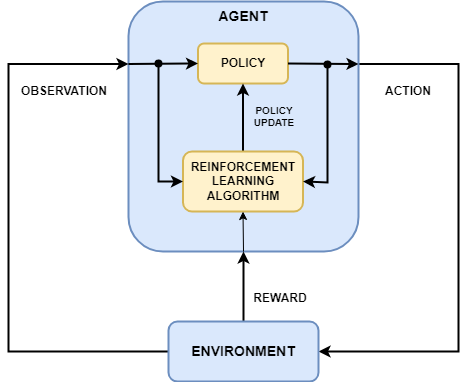
\includegraphics[width=8cm]{./Attachments/ReinforceModelDia.png}}
\caption{RL Process Diagram illustrating the interaction between the Agent and Environment.}\label{fig:ReinforceModelDia}
Source:
\href{https://www.mathworks.com/help/reinforcement-learning/ug/what-is-reinforcement-learning.html} {https://www.mathworks.com/help/reinforcement-learning/ug/what-is-reinforcement-learning.html}
\end{figure}

As shown in Figure \ref{fig:ReinforceModelDia}, the environment provides observations and rewards based on the agent’s actions, completing the learning loop. The reinforcement learning algorithm updates the policy to favor actions that lead to higher expected rewards.

\subsubsection{Reinforcement Learning in Video Games}

In video games, RL enables agents to learn complex behaviors by trial and error, without the need for manually scripted rules. For instance, in a 2D platformer environment, the agent may learn to walk, jump, dash, avoid enemies, and collect items. The state might include the player’s position, velocity, health status, or proximity to obstacles. Actions could involve movement directions or ability triggers, and rewards can be tied to reaching checkpoints, avoiding damage, or completing levels.

\subsubsection{Temporal Credit Assignment}

One unique aspect of RL is handling delayed rewards. Agents must learn to associate long-term outcomes with earlier decisions, a challenge known as the temporal credit assignment problem. For example, a jump executed early in a level may lead to avoiding death several seconds later, and the RL system must discover that causal link through repeated exploration.

\subsubsection{Exploration vs. Exploitation}

A fundamental challenge in RL is the trade-off between exploration (trying new actions to discover rewards) and exploitation (choosing known actions that yield high rewards). Effective training strategies balance these two aspects to ensure the agent continues to discover optimal behaviors without getting stuck in local minima.

\subsubsection{Episode-Based Learning and Reset Logic}

RL training typically occurs across episodes, bounded simulations of gameplay that end upon success, failure, or time limit. After each episode, the environment is reset, allowing the agent to explore new sequences and refine its strategy over time.

These characteristics make RL an ideal candidate for training adaptive game agents that can handle non-deterministic conditions and learn effective strategies without explicit programming.

\section{Proximal Policy Optimization (PPO)}

Proximal Policy Optimization (PPO) is a reinforcement learning algorithm introduced by Schulman et al. \cite{schulman2017ppo} as a more efficient and practical alternative to earlier policy optimization methods such as Trust Region Policy Optimization (TRPO). PPO strikes a balance between theoretical robustness and implementation simplicity, making it highly suitable for complex and high-dimensional environments such as video games.

\subsubsection{Policy Gradient Methods and TRPO}

In standard policy gradient methods, the agent updates its policy by maximizing the expected return through gradient ascent. The surrogate objective for the policy gradient is given by:

\begin{equation}
\hat{g} = \mathbb{E}_t \left[ \nabla_{\theta} \log \pi_{\theta}(a_t | s_t) \hat{A}_t \right]
\end{equation}

Where:
\begin{itemize}
\item $s_t$: The state of the environment at time step $t$.
\item $a_t$: The action taken by the agent at time step $t$.
\item $\theta$: The parameter vector of the policy network (e.g., weights in a neural network).
\item $\hat{g}$: The estimated policy gradient. It determines the direction in which the policy parameters should be updated to improve expected rewards.
\item $\mathbb{E}t[\cdot]$: Expectation taken over timesteps $t$. This indicates that the gradient is averaged over a batch of sampled trajectories or steps.
\item $\nabla_{\theta}$: Gradient operator with respect to the policy parameters $\theta$.
\item $\pi_{\theta}(a_t | s_t)$: The stochastic policy. It defines the probability of taking action $a_t$ given the current state $s_t$ under the policy parameterized by $\theta$.
\item $\log \pi_{\theta}(a_t | s_t)$: The log-probability of selecting action $a_t$ in state $s_t$. This is used because its gradient provides an unbiased estimate for the policy update.
\item $\hat{A}_t$: The advantage estimate at time $t$, indicating how much better (or worse) an action is compared to the average performance at that state. A positive advantage encourages repeating the action, while a negative advantage discourages it.
\end{itemize}

While effective, naive gradient ascent may lead to excessively large updates that destabilize training. To address this, TRPO introduces a constraint based on the Kullback–Leibler (KL) divergence between the old and new policy distributions:

\begin{equation}
\max_{\theta} \ \mathbb{E}_t \left[ \frac{\pi_{\theta}(a_t \mid s_t)}{\pi_{\theta_{\text{old}}}(a_t \mid s_t)} \hat{A}_t \right] \quad \text{subject to} \quad \mathbb{E}_t \left[ KL\left[ \pi_{\theta_{\text{old}}}(\cdot \mid s_t) \,\|\, \pi_{\theta}(\cdot \mid s_t) \right] \right] \leq \delta
\end{equation}
\newpage
Where:
\begin{itemize}
\item $\theta$: Current parameters of the policy being optimized.
\item $\theta_{\text{old}}$: Parameters of the policy before the update (used as a baseline for measuring change).
\item $\pi_{\theta}(a_t \mid s_t)$: Probability of taking action $a_t$ in state $s_t$ under the current policy.
\item $\pi_{\theta_{\text{old}}}(a_t \mid s_t)$: Probability of taking the same action under the old policy.
\item $\hat{_A}t$: Estimated advantage function at time step $t$, which represents how much better or worse the taken action was compared to the average.
\item $\frac{\pi{\theta}(a_t \mid s_t)}{\pi_{\theta_{\text{old}}}(a_t \mid s_t)}$: Importance sampling ratio (also known as the probability ratio), which corrects for the fact that data was collected under the old policy.
\item $\mathbb{E}t[\cdot]$: Expectation over time steps or sampled trajectories.
\item $KL[\cdot ,|, \cdot]$: Kullback–Leibler divergence, a measure of how different two probability distributions are.
\item $KL\left[ \pi{\theta_{\text{old}}}(\cdot \mid s_t) ,|, \pi_{\theta}(\cdot \mid s_t) \right]$: KL divergence between the old policy and the new policy at a given state. This measures how much the new policy has changed relative to the old one.
\item $\delta$: A small positive threshold (hyperparameter) that bounds how much the new policy is allowed to deviate from the old policy. It serves as a trust region constraint.
\end{itemize}

This formulation ensures that the policy improvement step does not shift the agent's behavior too drastically, which helps maintain stable and reliable learning. Although effective, TRPO's reliance on second-order optimization and the need to compute the KL divergence make it relatively difficult to implement and compute-intensive.

\subsubsection{Clipped Surrogate Objective}
PPO simplifies the TRPO constraint by introducing a clipped surrogate objective that approximates trust region behavior without explicitly computing second-order derivatives. The clipped objective is defined as:

\begin{equation}
L^{\text{CLIP}}(\theta) = \mathbb{E}_t \left[ \min \left( r_t(\theta) \hat{A}_t, \ \text{clip}\left(r_t(\theta), 1 - \epsilon, 1 + \epsilon\right) \hat{A}_t \right) \right]
\end{equation}

Where:
\begin{itemize}
\item $r_t(\theta) = \frac{\pi_{\theta}(a_t | s_t)}{\pi_{\theta_{\text{old}}}(a_t | s_t)}$: Probability ratio between the new and old policy.
\item $\epsilon$: Clipping threshold (typically 0.1 to 0.2) controlling how much the policy is allowed to change per update.
\end{itemize}

This objective penalizes updates that cause large policy shifts, effectively constraining updates within a small neighborhood of the old policy, thereby maintaining stability while encouraging learning progress.

\subsubsection{Combined Objective and Additional Terms}
The final PPO objective combines the clipped policy loss with additional components: a value function loss for accurate reward estimation and an entropy bonus to encourage exploration. The complete loss function is:

\begin{equation}
L^{\text{PPO}} = \mathbb{E}_t \left[ L^{\text{CLIP}}_t(\theta) - c_1 L^{\text{VF}}_t(\theta) + c_2 S[\pi_{\theta}](s_t) \right]
\end{equation}

Where:
\begin{itemize}
\item $L^{\text{CLIP}}_t(\theta)$: Clipped surrogate policy loss at time step $t$.
\item $L^{\text{VF}}_t(\theta)$: Squared error between predicted and target value estimates (value loss).
\item $S\pi_{\theta}$: Entropy of the policy at state $s_t$ to promote exploration.
\item $c_1$, $c_2$: Coefficients that control the weighting of the value loss and entropy bonus, respectively.
\end{itemize}


\subsection{Advantages and Suitability for Game Environments}

PPO has demonstrated high empirical performance in both discrete and continuous control problems, including benchmark environments like Atari and MuJoCo. Key advantages include:
\begin{itemize}
\item Simplicity of implementation using standard deep learning frameworks.
\item High training stability and robustness across different hyperparameters.
\item Suitability for environments with high-dimensional or stochastic observations.
\end{itemize}

In the context of this project, PPO is used to train adaptive agents for 2D platformer games, where actions such as jumping, dashing, and avoiding hazards require both temporal coordination and spatial awareness. PPO’s clipping mechanism ensures that learning is stable and reliable, even in complex environments with diverse platforming mechanics and variable reward structures.

\section{Development Tools}

\subsection{Unity}
Unity is a widely-used game engine known for its support of both 2D and 3D game development, offering an extensive suite of tools for scene design, animation, physics, and cross-platform deployment. It provides a modular component-based architecture, enabling rapid prototyping and flexible gameplay development. Unity's support for custom scripting, asset import pipelines, and a rich ecosystem of packages makes it particularly well-suited for game AI experimentation and deployment. The Unity Editor also includes built-in visualization, profiler, and debugging tools that facilitate game iteration and performance tuning.

\subsection{ML-Agents Toolkit}
The Unity ML-Agents Toolkit is an open-source machine learning library designed to bridge Unity and modern reinforcement learning algorithms. It allows game developers to embed intelligent behavior into their games using machine learning, particularly reinforcement learning (RL). The toolkit includes:
\begin{itemize}
\item A Python training backend that integrates with libraries such as PyTorch for model training.
\item A set of Unity-side C\# components to define agents, behaviors, and sensors.
\item Support for both visual and vector-based observations, discrete and continuous action spaces, and reward signal configuration.
\item Export capabilities to convert trained models into ONNX format for inference inside Unity runtime.
\end{itemize}
The toolkit is highly extensible and supports training with multiple agents simultaneously in a shared or parallelized environment.

\subsection{Python}
Python is a high-level programming language widely used in scientific computing, machine learning, and automation. In this context, Python serves as the main language for configuring, executing, and managing the training process of reinforcement learning agents. Key reasons for its use include:
\begin{itemize}
\item Compatibility with ML-Agents' training pipeline.
\item Integration with machine learning libraries such as PyTorch for neural network optimization.
\item Access to data processing tools like NumPy and Pandas, which are useful for monitoring and evaluating model performance.
\item TensorBoard support for visualizing training metrics, including rewards, episode length, and loss trends.
\end{itemize}

\subsection{C\#}
C\# is the primary programming language used within Unity for developing game logic, agent control scripts, UI systems, and custom components. Its integration into Unity's scripting API allows developers to:
\begin{itemize}
\item Control gameplay mechanics and interactions between objects.
\item Define behavior parameters for ML agents, including state tracking, sensor input, and action execution.
\item Implement physics-based movement, animation controllers, and in-game event handling.
\item Interface with Unity's MonoBehaviour system to manage game loop events such as initialization, updates, and collisions.
\end{itemize}
C\# provides a balance of performance and expressiveness, making it well-suited for real-time game development.

\subsection{ONNX Runtime}
ONNX (Open Neural Network Exchange) is an open standard format for representing machine learning models. After training reinforcement learning agents using the ML-Agents toolkit, the resulting models are exported in ONNX format. Unity supports ONNX model inference through the Barracuda inference engine, enabling:
\begin{itemize}
\item Embedding trained models directly into game builds for real-time AI decision-making.
\item Hardware-agnostic execution across different platforms (Windows, macOS, WebGL, etc.).
\item Seamless deployment without requiring Python or ML libraries at runtime.
\end{itemize}
ONNX provides a robust and portable way to integrate learning-based AI into production Unity games.

\subsection{Development Environment}
The development workflow combines multiple software tools to streamline programming, training, and testing:
\begin{itemize}
\item \textbf{Visual Studio:} Used for writing and debugging C\# scripts in Unity.
\item \textbf{Python Environment:} Managed through Anaconda or virtual environments to isolate dependencies required for ML-Agents.
\item \textbf{Git:} Used for version control, backup, and collaborative development.
\item \textbf{Unity Editor Tools:} Includes physics simulators, asset organization tools, and visual debugging aids.
\end{itemize}
These tools contribute to a structured and maintainable development pipeline from prototyping to deployment.

\section{Related research}

\subsection{Automated Playtesting in Game Development}
Playtesting is an important part of game development since it ensures that the challenges are balanced, systems work properly, and the player experience remains enjoyable. Traditionally, this process has relied on manual testers, which may be time-consuming and costly. In response to these issues, Sriram (2019)\cite {playtesting} researches the use of deep reinforcement learning (DRL) and curriculum learning to automate playtesting in 2D platformer games. His research introduces an Automated Playtesting (APT) program that trains AI agents to explore game levels, discovering design defects and gameplay imbalances without the need for operator input. By gradually increasing level complexity, these AI agents learn to adapt and manage a wide range of in-game events, making them useful for assessing new levels.\par
\begin{figure}[!h]
\centering
\fbox{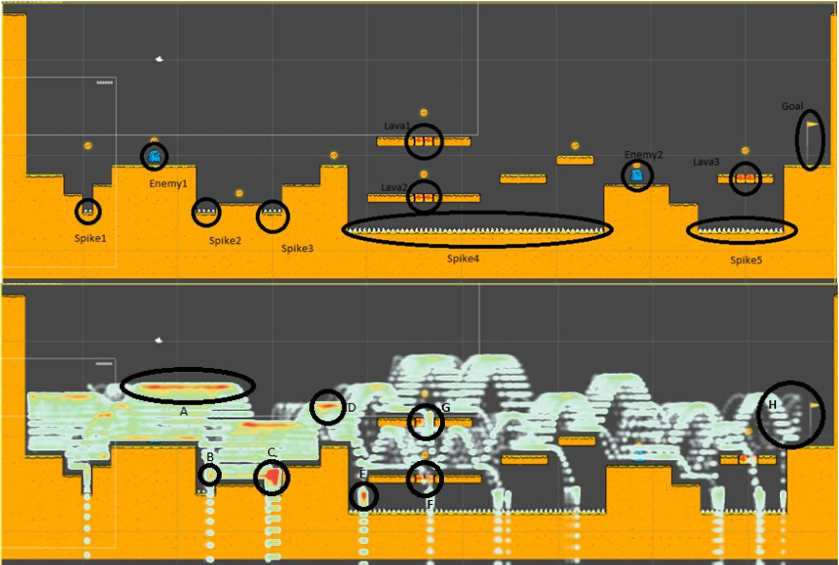
\includegraphics[width=10cm]{./Attachments/Automatebugtest.png}}
\caption{Unseen level and Unseen level with the agent heat map}\label{fig:UnseenLevel}
Source:
\href{https://repository.library.northeastern.edu/files/neu:m0455c95d/fulltext.pdf}{https://repository.library.northeastern.edu/files/neu:m0455c95d/fulltext.pdf} 
\end{figure}
Sriram's methodology provides a data-driven strategy for playtesting, but it is not the only option. Scripted AI agents are a more traditional approach, as they follow specific rules and behaviors rather than learning flexibly. These bots are easier to implement and use far less computational resources. However, they lack flexibility, which means they cannot generalize well across game levels or detect unexpected gameplay problems. In comparison, DRL-based playtesting is a versatile and scalable method that is especially helpful for games with automated generation or advanced level designs.\par
\newpage
\subsection{AI Techniques in 2D Platformer Games}
AI is an important tool for creating interesting yet challenging gameplay, particularly in platform games. In this area, AI behavior greatly influences player interest and difficulty. To improve AI behavior, Persson (2005)\cite {platformer_ai} studies three AI methods: pathfinding, image recognition, and line of sight. Their research focuses on AI movement and perception for more realistic interactions. The detection of line of sight ensures that the opponents will never see the player unless there are no obstacles in their path, preventing their irrational behavior. If they see changes in their environment with the aid of image recognition, then the AI will make appropriate changes to their actions. Finally, pathfinding algorithms enable AI to traverse complex levels, allowing for accurate movement while following or avoiding players.\par
\begin{figure}[!h]
\centering
\fbox{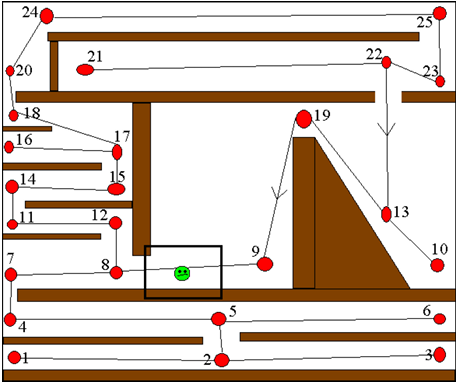
\includegraphics[width=10cm]{./Attachments/AITechniquesin2DPlatformerGames.png}}
\caption{In a 2D platform game, pathfinding nodes are shown as ellipse with corresponding indexes and connections on the map.}\label{fig:AITechniq}
Source:
\href{https://www.diva-portal.org/smash/get/diva2\%3A4762/FULLTEXT01.pdf?utm\_source=chatgpt.com}{https://www.diva-portal.org/smash/get/diva2\%3A4762/FULLTEXT01.pdf?utm}
\end{figure}
Behavior trees and FSMs make for an alternative pseudo-scientific contrast, they would be a fit in the context of game AI. FSMs provide a fixed, predictable AI behavior strategy, tending to have an extraordinarily rigid structure that requires much tuning to reproduce complex interactions. Behavior trees are about modularity and scalability, but still, they lack dynamically generated structures for decision making. Persson's solution offers a system that is more dynamic in character than pure FSM-based behavior systems but suffers from a downslope in computation.\par
\newpage
\subsection{Pathfinding and Navigation in Platformer AI}
One main issue within platformer AI is making an intelligent movement deemed natural and responsive. Smith (2021)\cite{physics_pathfinding} has proposed a physics-based pathfinding system that moves AI-controlled characters with a real-life dynamic principle for level navigation. The construction of a platform graph is established, with surfaces as nodes and possible movement trajectories as edges. AI agents use the A* pathfinding algorithm to determine optimal routes between platforms following the physics enforced by the game. This is not pure AI control since Smith's system translates movement decisions into simulated player inputs to guard against jerkiness and make motions feel natural.\par
\begin{figure}[!h]
\centering
\fbox{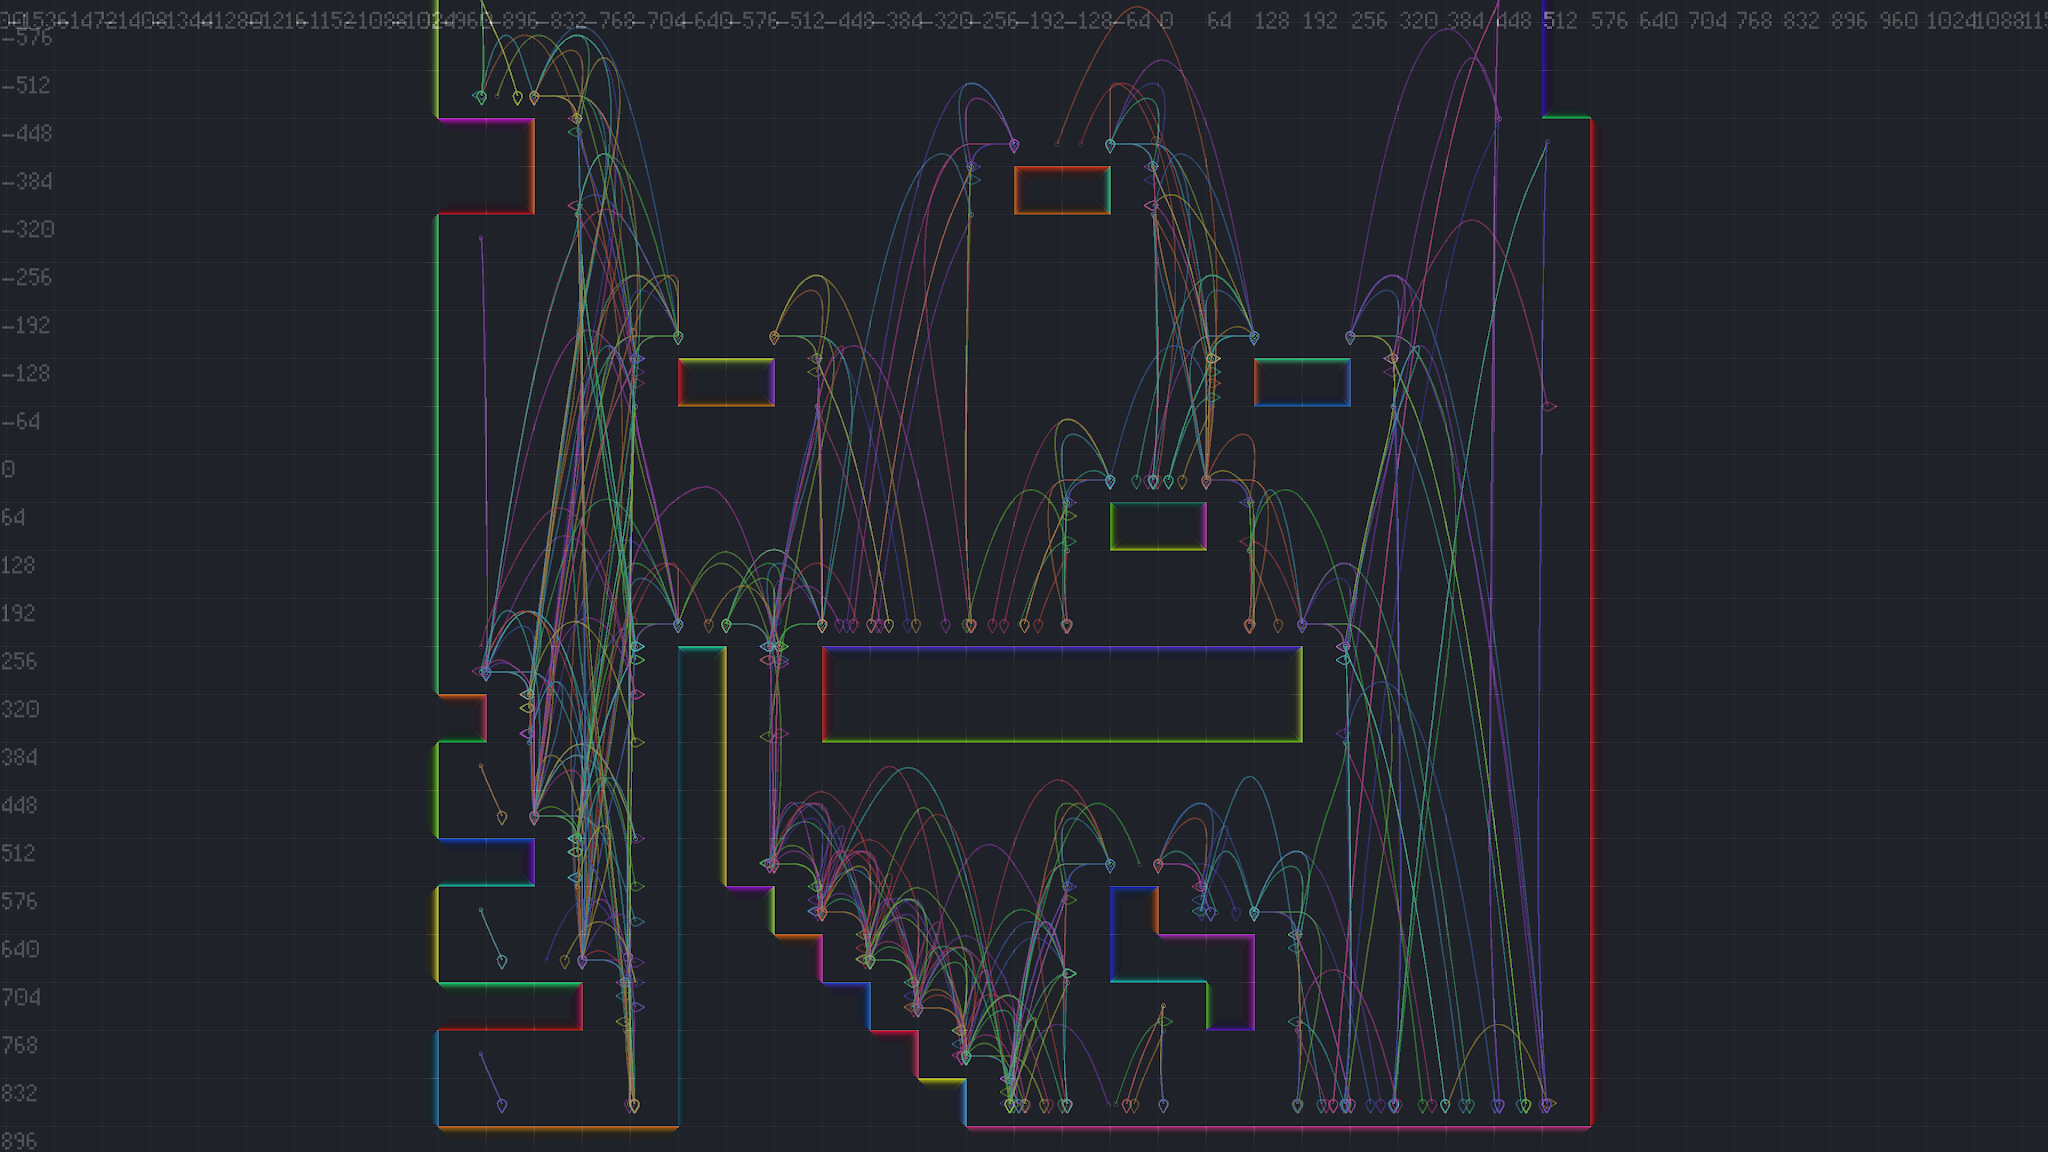
\includegraphics[width=10cm]{./Attachments/PathfindingandNavigationinPlatformerAI.png}}
\caption{Using A* search to find path through the graph}\label{fig:A*tofindPath}
Source:
\href{https://devlog.levi.dev/2021/09/building-platformer-ai-from-low-level.html?utm\_source=chatgpt.com}{https://devlog.levi.dev/2021/09/building-platformer-ai-from-low-level.html?utm\_source=chatgpt.com}  
\end{figure}
Smith's algorithmic approach, in contrast to machine learning-based navigation systems, allows for a greater degree of control and responsiveness. However, it is still limited. Deep reinforcement learning (DRL) would be an alternative approach to AI navigation, where agents would learn movement strategies through trial and error. On the one hand, the advantage of DRL-based AI is its adaptation to a dynamically changing environment; this, of course, comes alongside their requirement of extensive training and computation resources. Smith's method, conversely, is fast and reliable during runtime, for their physics-based paths are pre-calculated, yet they lack the adaptability of AI solutions based on DRL to tackle the unforeseen changes of levels.\par
\newpage
\section{Gap Analysis}
While artificial intelligence has made notable strides in 2D platformer games, several recurring limitations remain evident across the literature. For instance, in Sriram’s (2019) project on automated playtesting using reinforcement learning, the AI agent was trained to navigate platformer levels for the purpose of validating level design. Although the study effectively showcased how deep reinforcement learning (DRL) can be applied in testing environments, the focus remained on single-agent behavior in relatively static and simplified levels. There was no interaction with dynamic enemies or evolving objectives, and the system lacked the flexibility to handle more diverse or unpredictable challenges, conditions often present in real gameplay.Similarly, Persson (2005) presented a foundational overview of traditional AI techniques in 2D platformers, including pathfinding, line-of-sight mechanics, and behavior trees. These techniques were, and still are, widely used due to their efficiency and ease of implementation. However, they rely on rule-based logic, which tends to produce predictable and rigid behavior. These systems often fail to generalize well when faced with new level structures or gameplay rules, limiting their usefulness in adaptive game environments or procedural content systems.Smith (2021) explored physics-based pathfinding using A* algorithms and platform graphs, providing a practical method for navigating complex 2D spaces. His work contributes valuable insights into deterministic path planning, especially in tightly constrained levels. However, this approach assumes a largely fixed environment and doesn’t incorporate learning or adaptation over time. As a result, agents guided solely by static pathfinding algorithms struggle when unexpected gameplay changes occur, such as moving platforms, adversarial agents, or real-time hazards.Taken together, these studies highlight a clear opportunity for improvement: while each offers effective strategies for solving specific problems, they often fall short in handling dynamic gameplay, adapting to new challenges, or interacting with other agents. This is where our work seeks to contribute, by creating a reinforcement learning-driven framework that not only learns from experience but also adapts to a variety of gameplay elements through a modular, generalizable design.
\section{How our work differs}
This project builds upon the knowledge gained from the previous research while addressing the shortcomings of that research through a somewhat novel mixture of reinforcement learning, adversarial agent design, and modular asset creation. Sriram’s (2019) work was specific to the use of a single agent to automatically validate levels; this work instead looks at having two agents interact within an environment, both the player and the enemy agent are being trained together. Such an adversarial setup makes things more complicated and realistic from the perspective of the agent and thus allows for a richer framework for gameplay-testing and behavior emergence.
Our approach stands several other feet taller than Persson’s (2005) rule-based ones as it puts Proximal Policy Optimization (PPO) to work to allow agent training from scratch using feedback from the environment while being more adaptive and functioning under some measures of uncertainty. This design choice of switching from hard-coded behavior to trainable policies vastly improves an agent’s ability to function in procedurally varied or evolving levels.While Smith (2021) deals with deterministic navigation, what we have here is an integration of physics-aware decision-making into a learning framework, wherein an agent can compute a path but is also able to revise its traversal policy depending on the outcomes and depending on interactions with moving obstacles or enemies. Another major innovation is a modular and reusable asset design. In contrast to many prior approaches that custom-build AI systems for specific games or sets of use cases, this platformer AI is designed to be a stand-alone Unity asset, which can be plugged into all kinds of 2D games with very few modifications. This is, thus, a goldmine for indie developers and researchers.


% Can define this in the preamble..
%You can place the figure and refer to it as Figure~\ref{fig:model2}.
%The figure and table numbering will be run and updated automatically when you add/remove tables/figures from the document.

%\begin{figure}[!h]\centering
%\setlength{\fboxrule}{0.2mm} % can define this in the preamble
%\setlength{\fboxsep}{1cm}
%\fbox{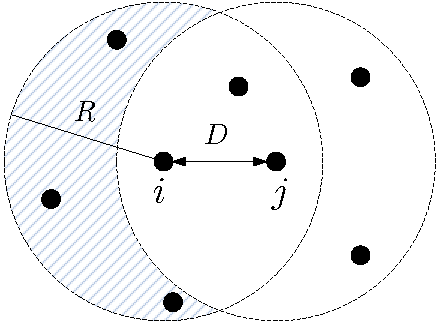
\includegraphics[width=5cm]{./model2.pdf}}
%\caption{The network model}\label{fig:model2}
%\end{figure}

%%%%%%%%%%%%%%%%%%%%%%%%%%%%%%%%%%%%%%%%%%%%%%%%%%%%%55
%%%%%%%%%%%%%%%%%%%%%%%%%%%%%%%%%%%%%%%%%%%%%%%%%%%%%
%%%%%%%%%%%%%%%%%%%%%%%%%%%%%%%%%%%%%%%%%%%%%%%%%%%%%
\chapter{Methodology And Design}

\section{Introduction}

This chapter outlines the methodology and design principles employed in the development of an adaptive artificial intelligence (AI) system tailored for 2D platformer games. The project integrates reinforcement learning into a modular AI framework, aiming to provide a reusable and easily extendable solution for game developers.\par

Building on the theoretical foundations established in the previous chapter, this section focuses on the practical aspects of system implementation. The goal is to bridge academic research in reinforcement learning with real-world game development tools and workflows. To achieve this, a structured, modular design was adopted to ensure flexibility, reusability, and compatibility across different 2D platformer projects.\par

This chapter will outline the key components of our methodology, including:

\begin{itemize}
\item \textbf{System Architecture:} An overview of the core system components, including Unity, ML-Agents, and the communication pipeline between the training environment and the reinforcement learning algorithm.
\item \textbf{Game Environment Design:} A description of the custom 2D platformer environment developed for training and evaluating AI behavior.
\item \textbf{AI Agents Development:} The structure and modular design of the player agent, including its perception setup, action abstraction, and behavior controls.
\item \textbf{AI Algorithms and Models:} The selection and application of Proximal Policy Optimization (PPO) as the learning algorithm.
\item \textbf{Training Process and Optimization:} Training setup, reward shaping strategies, curriculum learning stages, and monitoring tools.
\item \textbf{AI Integration and Packaging:} The deployment of the trained model into Unity for inference, along with steps for packaging and delivering it as a reusable Unity asset.
\end{itemize}

By following this methodology, the project aims to deliver a robust AI development framework that supports intelligent agent behavior, simplifies the adoption of reinforcement learning in indie projects, and lays the groundwork for future scalability and customization.
%Explain the design (how you plan to implement your work) of your project. Adjust the section titles below to suit the types of your work. Detailed physical design like circuits and source codes should be placed in the appendix.

\section{System Architecture}

The architecture of this project is designed to support modular, trainable reinforcement learning agents within a Unity-based 2D platformer game. It integrates Unity ML-Agents, a dual-camera perception system, custom action middleware, and a structured feedback loop for learning. The primary goal is to provide a scalable and adaptable framework that can be reused across various platformer game scenarios. Figure \ref{fig:TrainingArchitecture} illustrates the complete learning system.

\begin{figure}[H]
\centering
\fbox{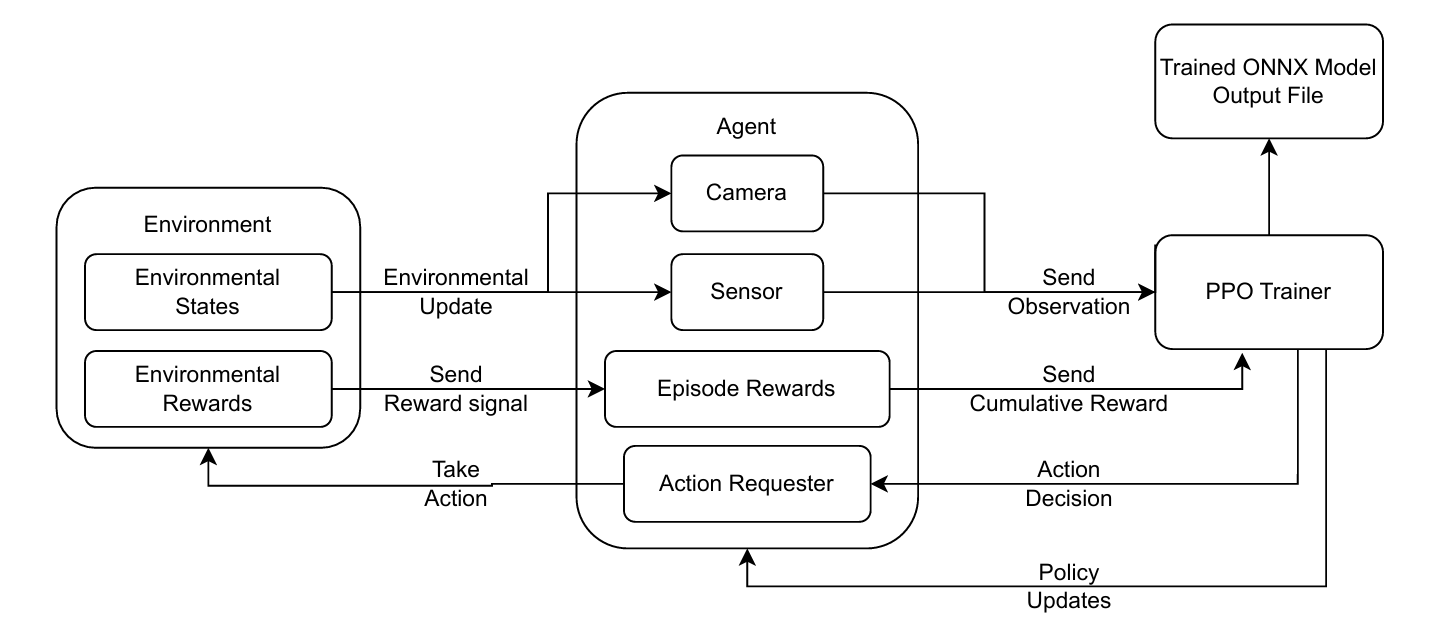
\includegraphics[width=14cm]{./Attachments/SystemDiagramNew.png}}
\caption{System Architecture and Reinforcement Learning Training Loop}\label{fig:TrainingArchitecture}
\end{figure}

\subsection{Component Overview}

\begin{itemize}
\item \textbf{Environment:} The game world is created using Unity’s 2D tools, featuring platformer elements such as platforms, hazards, coins, and checkpoints. The environment continuously updates based on the agent’s actions and physics rules.

\item \textbf{Agent:} The agent acts as the decision-making entity. It receives environmental states or camera observations and interacts with the world through a policy network trained using PPO. Its action requests are routed through a modular Action Requester layer.

\item \textbf{Sensor and Camera:} The agent receives observations via attached sensors. In visual training scenarios, a secondary camera renders a simplified, color-coded version of the environment exclusively for the agent. This visual feed is passed as input to the model to guide decision-making.

\item \textbf{Action Requester:} This middleware abstracts the communication between the model’s outputs and the actual in-game behaviors. It converts action indices into commands (e.g., jump, dash) and delegates them to appropriate character controller components. The character controller then executes the received commands, updating the agent's position, animation, and interaction within the game environment.

\item \textbf{Reward System:} A reward handler observes events like reaching goals, collecting items, taking damage, or idling. These trigger scalar feedback signals that are sent back to the model to guide future learning.

\item \textbf{Episode Feedback Loop:} The ML-Agents framework calculates the cumulative reward per episode. At the end of each episode, the agent's performance is logged, and training resets begin from a new randomized state.

\item \textbf{PPO Trainer:} Training occurs on an external Python environment using Unity ML-Agents. The PPO trainer optimizes the policy parameters to improve the agent’s decision-making over time.

\item \textbf{ONNX Model Export:} Once trained, the resulting neural policy is exported in ONNX format and deployed back into Unity for inference. This makes the model reusable across different platformer environments without additional training.
\end{itemize}

\subsection{System Highlights}

This architecture emphasizes:
\begin{itemize}
\item Decoupled design for modularity and extensibility
\item Real-time reward feedback for adaptive learning
\item Dual-camera support for efficient agent perception
\item Seamless transition between training and inference modes
\end{itemize}

The structured pipeline facilitates experimentation, debugging, and deployment, ensuring that the agent can be reused and adapted in other projects by indie developers or game designers without machine learning expertise.

\section{Game Environment Design}
The game environment constitutes the primary interactive space in which reinforcement learning (RL) agents are trained and evaluated. A well-structured environment is critical to effective agent learning, as it defines the sensory inputs, action possibilities, feedback mechanisms, and contextual challenges that guide behavioral adaptation. This section elaborates on the structure, components, and mechanics of the custom 2D platformer environment used for this study, with emphasis on level design, agent interaction capabilities, physics implementation, and system validation.
\subsection{Level Structure and Composition}
The environment is designed as a 2D platformer world, incorporating fundamental elements commonly found in platformer games, such as platforms, obstacles, hazards, collectibles, and enemies. The level is structured to balance exploration, platforming challenges, and enemy encounters, ensuring that the agent experiences a diverse range of situations during training.\par
\subsubsection{Platforming and Terrain}
The terrain system integrates a variety of platform types that influence agent decision-making and navigational strategies. Each terrain element contributes uniquely to the richness of the training experience:
\begin{itemize}
\item  \textbf{Wall Surfaces:} Walls allow for interactions such as wall jumps or wall slides, affecting navigation strategies.
\item  \textbf{Solid Platforms:} Standard ground elements on which the agent can walk and jump.
\begin{figure}[H]
\centering
\fbox{
\includegraphics[width=5cm]{./Attachments/SolidPlat.png}}
\caption{The image shows solid wall and platform.}\label{fig:SolidPlat}
\end{figure}
\item  \textbf{One-Way Platforms:} Platforms that can be landed on from above but allow the agent to jump through from below.
\begin{figure}[H]
\centering
\fbox{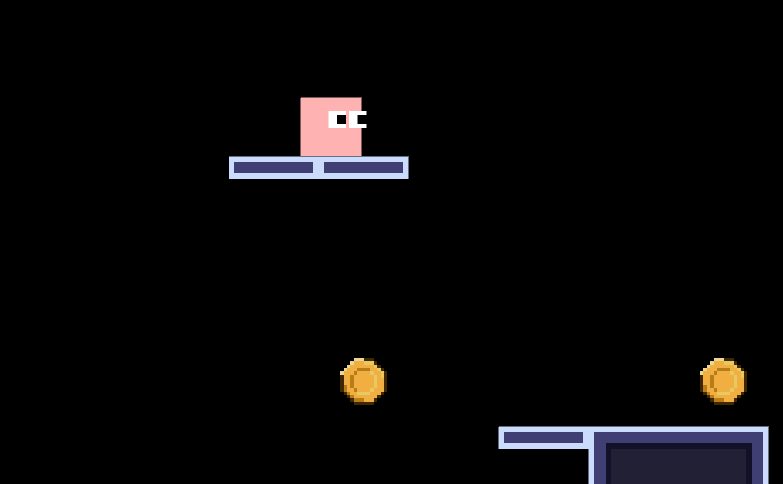
\includegraphics[width=5cm]{./Attachments/OneWayPlat.png}}
\caption{The image highlights one-way platforms.}\label{fig:OneWayPlat}
\end{figure}
\item  \textbf{Moving Platforms:} Dynamic platforms that require precise timing and positioning.
\begin{figure}[H]
\centering
\fbox{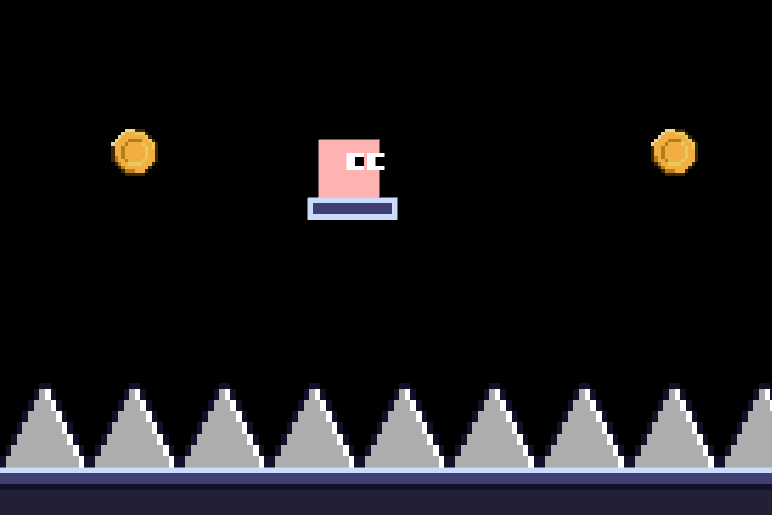
\includegraphics[width=5cm]{./Attachments/MovingPlat.png}}
\caption{The image highlights moving platforms over obstacle.}\label{fig:MovingPlat}
\end{figure}
\end{itemize}
\subsubsection{Interactive Elements}
To enrich the environment's interactivity and encourage exploration, a range of functional objects are distributed throughout the level:
\begin{itemize}
\item  \textbf{Goals:} Objects such as coins or checkpoints that act as positive reinforcement signals for the agent.
\begin{figure}[H]
\centering
\fbox{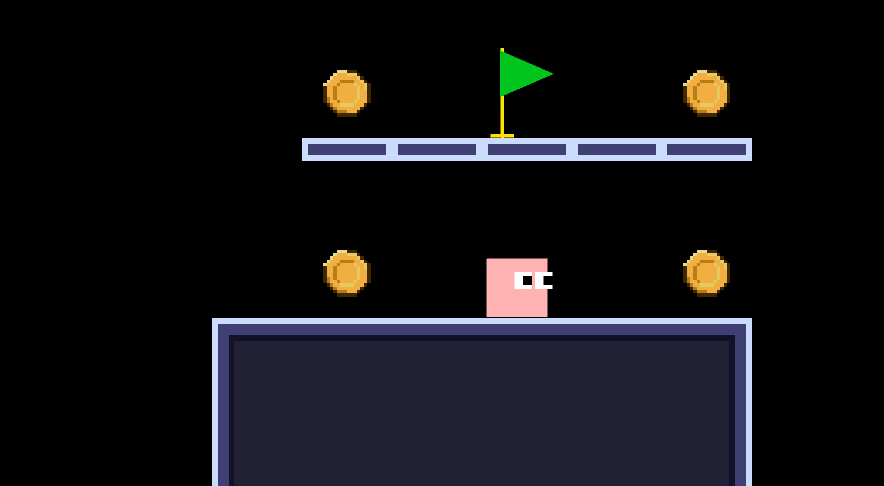
\includegraphics[width=5cm]{./Attachments/Goals.png}}
\caption{The image highlights coins and checkpoint as goals.}\label{fig:Goals}
\end{figure}
\item  \textbf{Hazards:} Spikes, traps, or pits that impose penalties and help the agent learn avoidance behaviors.
\begin{figure}[H]
\centering
\fbox{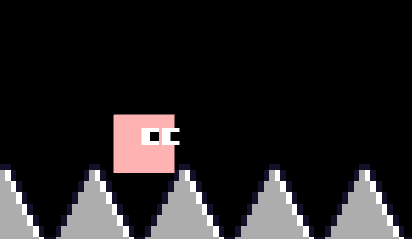
\includegraphics[width=5cm]{./Attachments/Hazards.png}}
\caption{The image highlights player falling into hazard.}\label{fig:Hazards}
\end{figure}
\item  \textbf{Enemies:} Opponents with basic AI that introduce combat-related decisions and temporal awareness.
\begin{figure}[H]
\centering
\fbox{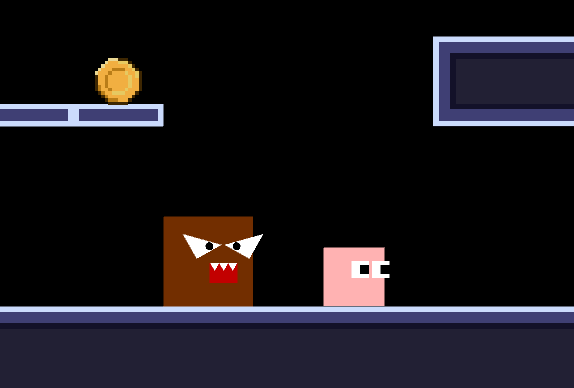
\includegraphics[width=5cm]{./Attachments/EnemyPic.png}}
\caption{The image highlights enemy chasing player.}\label{fig:EnemyPic}
\end{figure}
\end{itemize}
These elements are strategically placed to guide the agent’s learning, providing a structured environment that encourages skill acquisition through reinforcement learning.
\begin{figure}[H]
\centering
\fbox{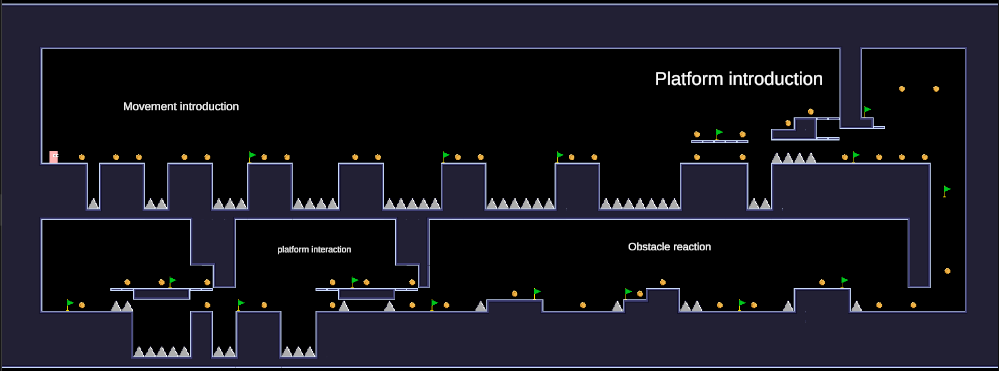
\includegraphics[width=10cm]{./Attachments/EnvironmentDesign.png}}
\caption{Environment Training Ground for the AI}\label{fig:EnvironmentDesign}
\end{figure}
\subsection{Agent Actions}
Table \ref{tbl:Agent Actions Table} outlines the available actions for Player and Enemy agents. These actions simulate the gameplay mechanics and ensure that the AI can engage with the environment and other agents meaningfully.
\begin{table}[H]
\caption{Agent Actions Table}\label{tbl:Agent Actions and Capabilities}
\begin{tabular}{|l|l|l|} \hline
& \textbf{Player Agent} & \textbf{Enemy Agent} \\ \hline
Actions & Walk and run & Walk and run \\ 
& Jump & Jump \\ 
& Attack (Melee) & Attack player (Melee)  \\ 
& Drop Down &  \\
& Dash &  \\ \hline
\end{tabular}
\end{table}
\subsubsection{Player Agent Actions}
\begin{itemize}
\item  \textbf{Walk and run:} Allows navigation of horizontal spaces.
\item  \textbf{Jump:} Essential for crossing gaps and reaching elevated platforms.
\item  \textbf{Attack (Melee):} Simulates combat mechanics where the player can engage with enemies or break objects.
\item  \textbf{Drop Down:} Enables traversal through one way platform accessing other places.
\item  \textbf{Dash:} Enables moving horizontally at a higher speed avoiding obstacles.
%\item  \textbf{Crouch:} Enables traversal through tight spaces or avoidance of overhead obstacles.%
\end{itemize}
\subsubsection{Enemy Agent}
\begin{itemize}
\item  \textbf{Walk and run:} Supports patrol or chase behaviors.
\item  \textbf{Jump:} Ensures enemies can traverse complex terrains.
\item  \textbf{Attack (Melee):} Adds combat mechanics, making the environment more dynamic.
%\item  \textbf{Crouch:} Enables traversal through tight spaces or avoidance of overhead obstacles.%
\end{itemize}
\subsection{Physics and Movement Constraints}
The movement and interaction mechanics of the game are governed by Unity’s built-in 2D physics engine, facilitated by the Rigidbody2D component and customized through script-based motion logic. This configuration enables realistic yet controllable movement responses, ensuring that the AI agent operates under consistent physical constraints. These constraints are crucial for promoting transferable behavior and narrowing the simulation-to-reality gap in reinforcement learning.

\subsubsection{Movement Mechanics}
Movement in the platformer environment is handled through a centralized input-processing system defined in the \texttt{HandleInput()} method of the \texttt{BasicPlayerMovement.cs} script. This function maps user or agent decisions into stateful input variables that drive the player’s actions across update cycles. Input is only processed when \texttt{inputEnabled} is set to true, ensuring synchronization between AI control and gameplay flow. 

\begin{lstlisting}[language={[Sharp]C}]
private void HandleInput()
{
	if (!inputEnabled) return;

	moveInput = new Vector2(Input.GetAxisRaw("Horizontal"), Input.GetAxisRaw("Vertical"));
	moveDir = moveInput.x;
	dropInput = moveInput.y;
	jumpInput = Input.GetKeyDown(KeyCode.Space);
	dashInput = Input.GetKeyDown(KeyCode.LeftShift);

	if (jumpInput)
	{
		Jump();
	}
	
	if (dashInput)
	{
		Dash();
	}
}
\end{lstlisting}
This method collects directional input using Unity's built-in \texttt{Input.GetAxisRaw()} system and stores it in the \texttt{moveDir} and \texttt{dropInput} variables. Action-based inputs such as jumping and dashing are mapped to boolean flags, \texttt{jumpInput} and \texttt{dashInput}, respectively. These are then passed to their corresponding methods (\texttt{Jump()} and \texttt{Dash()}) to initiate action events. This separation of input and behavior logic allows the system to be easily extended for reinforcement learning agents, which can override these inputs through scripted or neural decisions.

\begin{itemize}
\item  \textbf{Walking and Running:} Horizontal movement is applied using an acceleration-based force model. As shown in the \texttt{HandleMovement()} method which takes in one argument, \texttt{direction}, the lateral velocity is updated using player input and smoothed via velocity power with the following code snippet.
\begin{lstlisting}[language={[Sharp]C}]
private void HandleMovement(float direction)
{
	if (IsDashing) return;

	if (playerAttack == null || !playerAttack.isAttacking)
	{
		if (direction > 0 && !IsFacingRight)
			Flip();
		else if (direction < 0 && IsFacingRight)
			Flip();
	}

	float targetSpeed = direction * moveSpeed;
	float speedDifference = targetSpeed - rb.linearVelocity.x;
	float accelRate = (Mathf.Abs(targetSpeed) > 0.01f) ? acceleration : decceleration;
	float movement = Mathf.Pow(Mathf.Abs(speedDifference) * accelRate, velPower) * Mathf.Sign(speedDifference);

	if (!IsWallJumping)
	{
		rb.AddForce(movement * Vector2.right);
	}
	else
	{
		rb.linearVelocity = Vector2.Lerp(rb.linearVelocity, (new Vector2(direction * moveSpeed, rb.linearVelocity.y)), wallJumpLerp * Time.deltaTime);
	}
}
\end{lstlisting}
\item  \textbf{Jumping:} The \texttt{PerformJump()} and \texttt{HandleJump()} methods handle vertical jumping, including coyote time and jump buffering. When a jump is triggered, vertical velocity is reset and overridden:
\begin{lstlisting}[language={[Sharp]C}]
private void HandleJump()
{
	canJump = CanJump();
	canWallJump = CanWallJump();

	if (Time.time - lastJumpPressedTime <= jumpBufferTime)
	{
		if (canJump && !hasJumped)
		{
			PerformJump();
			hasJumped = true;
		}
		else if (canWallJump && !hasWallJumped)
		{
			wallJumpDir = (IsOnRightWall) ? -1 : 1;
			PerformWallJump(wallJumpDir);
			hasWallJumped = true;
		}
	}
}
\end{lstlisting}
\begin{lstlisting}[language={[Sharp]C}]
private void PerformJump()
{
	lastGroundedTime = 0;
	lastJumpPressedTime = 0;
	lastJumpTime = Time.time;
	rb.linearVelocity = new Vector2(rb.linearVelocity.x, 0f);
	rb.linearVelocity = new Vector2(rb.linearVelocity.x, jumpForce);
	isJumping = true;
}
\end{lstlisting}
This guarantees consistent jump height and reduces variance in vertical behavior, which is beneficial for stable learning outcomes.
\item  \textbf{Dashing:} Dash behavior is implemented via a coroutine in \texttt{PerformDash()}, where gravity is temporarily disabled and horizontal velocity is set explicitly which is handled by \texttt{HandleDash()}:
\begin{lstlisting}[language={[Sharp]C}]
private void HandleDash()
{
	if (CanDash() && lastDashPressedTime > lastDashTime)
	{
		StartCoroutine(PerformDash());
	}
}
\end{lstlisting}
\begin{lstlisting}[language={[Sharp]C}]
private IEnumerator PerformDash()
{
	isDashing = true;
	lastDashPressedTime = Time.time;
	dashDirection = IsFacingRight ? Vector2.right : Vector2.left;
	rb.gravityScale = 0;
	rb.linearVelocity = dashDirection * dashSpeed;
	yield return new WaitForSeconds(dashDuration);
	rb.gravityScale = gravityScale;
	isDashing = false;
	lastDashTime = Time.time;
}
\end{lstlisting}
This mechanic enables burst-based directional movement, adding timing complexity and escape strategies to the agent’s behavior model.
\item  \textbf{Wall Interactions:} Wall detection and sliding are handled in \texttt{HandleWallDetection()} and \texttt{HandleWallSlide()}. When the agent is airborne and collides with a vertical surface, its vertical descent is controlled:

\begin{lstlisting}[language={[Sharp]C}]
private void HandleWallSlide()
{
	if (IsOnWall && !IsGrounded && rb.linearVelocity.y < 0)
	{
		rb.linearVelocity = new Vector2(rb.linearVelocity.x, -wallSlideSpeed);
	}
}
\end{lstlisting}

In addition, wall jumping is enabled through the \texttt{PerformWallJump()} method. When the agent is near a wall and a jump input is received, a directional impulse is applied, launching the agent away from the wall. The direction is based on wall contact (left or right) and is calculated as follows:
\begin{lstlisting}[language={[Sharp]C}]
	private void PerformWallJump(int dir)
	{
		if (isWallJumping || hasWallJumped) return;
		
		lastGroundedTime = 0;
		lastJumpPressedTime = 0;
		rb.linearVelocity = Vector2.zero;
		Vector2 force = new Vector2(wallJumpForce.x, wallJumpForce.y);
		force.x *= dir;
		
		if (Mathf.Sign(rb.linearVelocity.x) != Mathf.Sign(force.x))
			force.x -= rb.linearVelocity.x;
			
		if (rb.linearVelocity.y < 0)
		{
			force.y -= rb.linearVelocity.y;
		}
		
		rb.AddForce(force, ForceMode2D.Impulse);
		isWallJumping = true;
		hasWallJumped = true;
	}
\end{lstlisting}
This mechanic increases vertical navigation flexibility and enables the agent to escape corners or ascend narrow shafts, enriching both player and AI-controlled movement strategies.
\end{itemize}
\subsubsection{Collision and Interaction System}
Unity’s physics engine and collider components are used to detect and manage interactions between the agent and the environment. These interactions are monitored continuously and affect the agent’s internal state and eligibility to perform actions.
\begin{itemize}
\item  \textbf{Ground and Wall Detection:} Performed via a box collider in \texttt{HandleGrounded()} and \texttt{HandleWallDetection}, these checks are used to determine whether the agent can initiate jumps, wall-jumps, or dash. The logic employs \texttt{Physics2D.OverlapBox()} and updates state variables accordingly:

\begin{lstlisting}[language={[Sharp]C}]
private void HandleGrounded()
{
	isGrounded = Physics2D.OverlapBox(_groundCheckPoint.position, _groundCheckSize, 0, _groundLayer) != null;

	if (isGrounded && !wasGrounded)
	{
		hasJumped = false;
		hasWallJumped = false;
		isJumping = false;
		isWallJumping = false;
	}

	if (isGrounded && rb.linearVelocityY <= 0)
	{
		lastGroundedTime = Time.time;
	}

	wasGrounded = isGrounded;
}
\end{lstlisting}
\begin{lstlisting}[language={[Sharp]C}]
private void HandleWallDetection()
{
	if (IsGrounded)
	{
		isOnWall = isOnLeftWall = isOnRightWall = false;
		return;
	}

	Transform leftCheck = IsFacingRight ? _wallCheckPointLeft : _wallCheckPointRight;
	Transform rightCheck = IsFacingRight ? _wallCheckPointRight : _wallCheckPointLeft;

	isOnLeftWall = Physics2D.OverlapBox(leftCheck.position, _wallCheckSize, 0, _wallLayer) != null;
	isOnRightWall = Physics2D.OverlapBox(rightCheck.position, _wallCheckSize, 0, _wallLayer) != null;

	isOnWall = IsOnLeftWall || IsOnRightWall;
	isWallJumping = false;
	hasWallJumped = false;
}
\end{lstlisting}
\begin{figure}[H]
\centering
\fbox{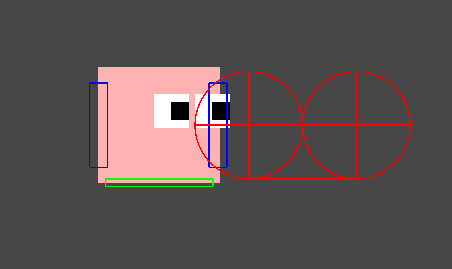
\includegraphics[width=5cm]{./Attachments/CollisionDetection.png}}
\caption{Collision detection and attack zone used in the player movement system.}\label{fig:CollisionDetection}
\end{figure}
\item  \textbf{Hazard Detection:} hazard detection is structured to operate via layer-based triggers and collisions (e.g., spikes or traps). These interactions would typically result in episode termination or reward penalties, and can be expanded through \texttt{OnCollisionEnter2D()} or \texttt{OnTriggerEnter2D()} events.

\begin{lstlisting}[language={[Sharp]C}]
private void OnTriggerEnter2D(Collider2D collision)
{
    if (collision.CompareTag("Hazard"))
    {
	Debug.Log("Player hit the spike (trigger)!");
	TakeDamage(maxHealth);
    }
}
\end{lstlisting}

\item  \textbf{Enemy Interaction:} Enemy detection and combat interactions are facilitated through the \texttt{PlayerAttack} script. These interactions allow for additional agent decision-making complexity, such as whether to evade or engage an enemy.
\end{itemize}
To further refine physical realism and training consistency, additional systems manage vertical acceleration and friction:
\begin{itemize}
\item \textbf{Custom Gravity:} The \texttt{ApplyCustomGravity()} method applies varying gravity multipliers depending on the jump state and vertical velocity. This produces more nuanced motion:
\begin{lstlisting}[language={[Sharp]C}]
rb.gravityScale = gravityScale * fallMultiplier;
\end{lstlisting}
\item \textbf{Friction Handling:} Friction is manually applied when movement input ceases, reducing velocity over time using impulses:
\begin{lstlisting}[language={[Sharp]C}]
rb.AddForce(Vector2.right * -amount, ForceMode2D.Impulse);
\end{lstlisting}
\end{itemize}

Through the combination of Unity physics components and finely tuned motion scripting, the agent operates within a physically constrained yet expressive movement model. This model serves as the foundation for learning transferable locomotion policies across varied level designs.

\subsection{Curriculum Learning Stages}

To improve training efficiency and agent generalization, a curriculum learning strategy is implemented. The idea is to start with simpler tasks and environments, gradually increasing complexity as the agent gains proficiency. This approach enables the reinforcement learning agent to learn fundamental behaviors incrementally rather than attempting to master all mechanics at once. The curriculum consists of four distinct stages, each introducing new gameplay concepts while building on previously acquired skills.

\subsubsection{Stage 1 – Basic Movement and Item Collection}

The initial stage introduces flat, single-layer environments designed to teach basic movement and reward-seeking behavior. The agent learns to:

\begin{itemize}
\item Move horizontally toward visible goals.
\item Collect coins or other positive-reward objects.
\item Avoid hazards such as spikes (present since this stage).
\end{itemize}

\begin{figure}[H]
\centering
\fbox{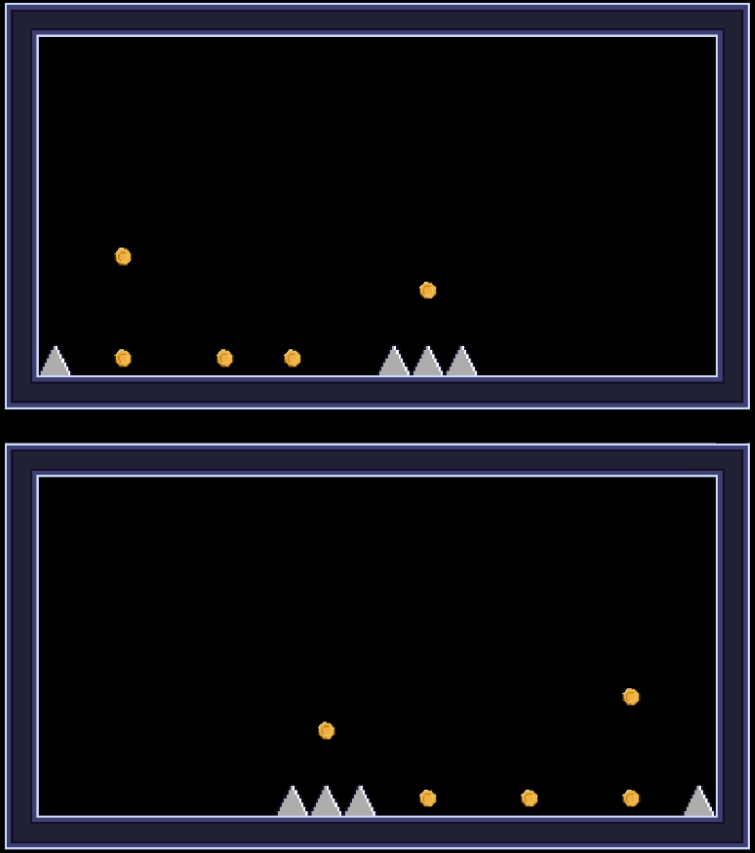
\includegraphics[width=5cm]{./Attachments/Stage1.png}}
\caption{Stage 1 – Basic Movement and Item Collection}\label{fig:Stage1}
\end{figure}

\subsubsection{Stage 2 – Advanced Navigation (Multi-layer Platforms)}

Once the agent consistently performs basic movement, multi-level environments are introduced. These levels feature vertical traversal requiring jumping. The agent learns to:

\begin{itemize}
\item Jump to elevated platforms and move vertically through the level.
\item Optimize paths through layered terrain to reach rewards.
\end{itemize}

\begin{figure}[H]
\centering
\fbox{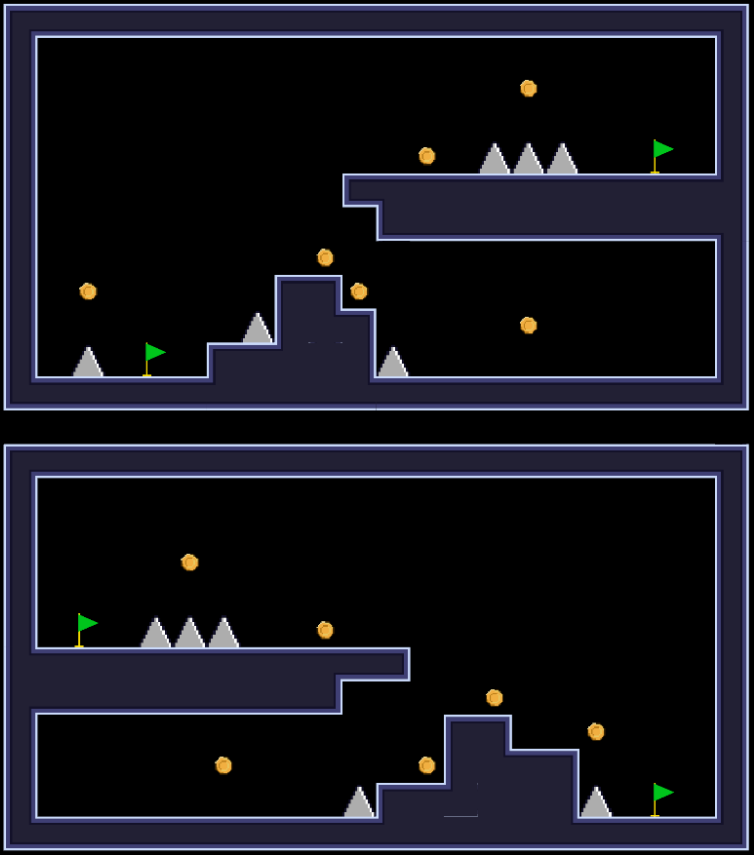
\includegraphics[width=5cm]{./Attachments/Stage2.png}}
\caption{Stage 2 – Advanced Navigation with Multi-layered Platforms}\label{fig:Stage2}
\end{figure}

\subsubsection{Stage 3 – One-Way Platform Introduction}

One-way platforms are added to introduce a new navigational rule. These platforms can be jumped onto from below and dropped through from above. The agent must learn to:

\begin{itemize}
\item Recognize one-way platforms as passable terrain.
\item Drop down through platforms when needed to reach goals or avoid hazards.
\item Adapt navigation strategy dynamically based on vertical positioning.
\end{itemize}

\begin{figure}[H]
\centering
\fbox{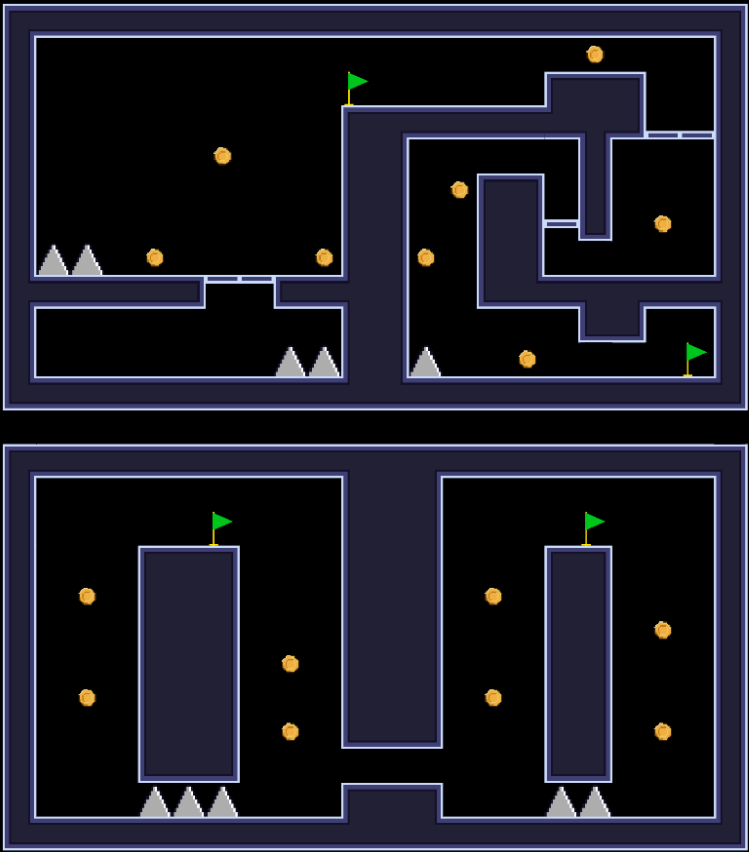
\includegraphics[width=5cm]{./Attachments/Stage3.png}}
\caption{Stage 3 – Introduction of One-Way Platforms}\label{fig:Stage3}
\end{figure}

\subsubsection{Stage 4 – Enemy Introduction and Combat Awareness}

In the final curriculum stage, basic enemy characters are introduced. These enemies follow simple state machine behavior (e.g., patrolling), and the agent must engage with or avoid them. New learning objectives include:

\begin{itemize}
\item Attacking enemies using melee actions.
\item Avoiding enemy attacks and contact.
\item Prioritizing combat versus avoidance depending on context.
\end{itemize}

\begin{figure}[H]
\centering
\fbox{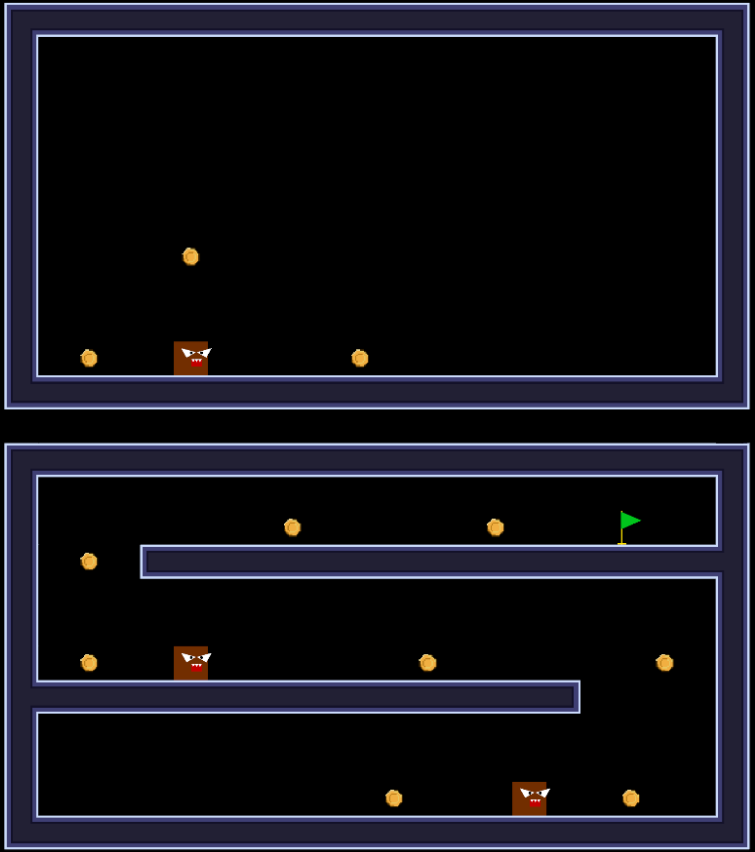
\includegraphics[width=5cm]{./Attachments/Stage4.png}}
\caption{Stage 4 – Enemy Introduction and Combat Interaction}\label{fig:Stage4}
\end{figure}

\subsubsection{Full-Scale Platformer Environment}

After completing all curriculum stages, the agent is transitioned to a large, hand-crafted platformer level designed to emulate real-world gameplay. This map includes all previously introduced mechanics—multi-layered platforms, one-way platforms, collectibles, hazards, and enemies—distributed throughout a complex and varied layout. This final training/testing stage serves to:

\begin{itemize}
\item Evaluate the agent’s ability to generalize behaviors learned from smaller curriculum stages.
\item Assess performance in realistic, high-difficulty scenarios involving dynamic decision-making.
\item Train on longer episodes with diverse routes, reward opportunities, and hazards.
\end{itemize}

\begin{figure}[H]
\centering
\fbox{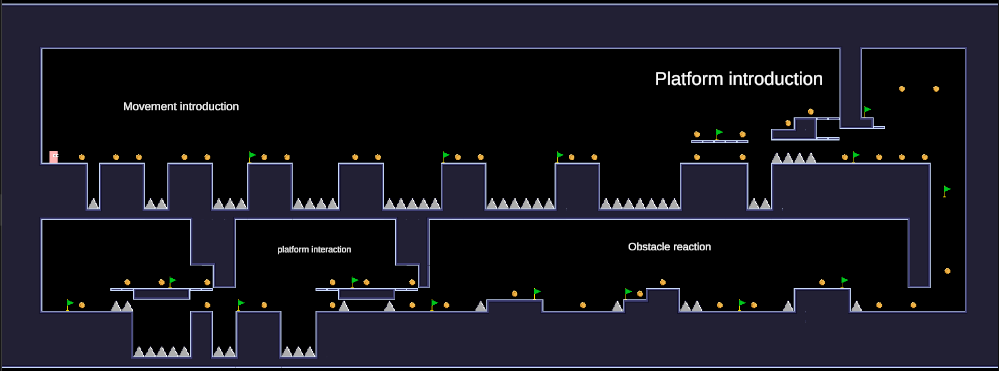
\includegraphics[width=12cm]{./Attachments/EnvironmentDesign.png}}
\caption{Full-Scale Environment for Final Training and Evaluation}\label{fig:FullLevel}
\end{figure}

This full environment is used for both extended training (with reward shaping) and testing the transferability of the agent’s skills. The layout simulates the kind of level design seen in commercial 2D platformer games, making it ideal for benchmarking the agent’s practical capabilities.

\subsection{Environment Testing}
Prior to integrating the reinforcement learning model, the platformer environment underwent systematic testing to ensure that it met the functional, performance, and scalability requirements necessary for stable agent training. These tests were essential for validating gameplay mechanics, maintaining frame rate stability, and ensuring compatibility with machine learning pipelines.
\subsubsection{Functional Testing}
Functional testing focused on verifying the correctness of the core gameplay systems. Using Unity’s play mode, scene inspector tools, and in-editor debugging outputs, the following aspects were evaluated:
\begin{itemize}
\item  \textbf{Movement Tests:} Confirmed that the agent could perform essential actions such as walking, jumping, dashing, and dropping through platforms, using the logic defined in the \texttt{BasicPlayerMovement} script.
\item  \textbf{Collision Tests:} Verified accurate collision detection with ground surfaces, hazards, enemies, and walls using Unity’s \texttt{Physics2D.OverlapBox()}.
\item  \textbf{Camera Tests:} Ensured the secondary ML-rendering camera captured a simplified, texture-free version of the environment to serve as the agent’s observation input.
\end{itemize}
\subsubsection{Scalability Testing}
To ensure the environment’s reusability across future projects and training scenarios, a series of scalability tests were conducted:
\begin{itemize}
\item  \textbf{Level Size Variability:} Different map sizes and segment arrangements were tested to validate agent adaptability across layouts.
\item  \textbf{Enemy and Obstacle Density:} The performance and behavior of agents were evaluated under varying densities of enemies and environmental hazards.
\item  \textbf{Generalization Potential:} Agents were tested in unseen level variants to assess their ability to transfer learned behaviors beyond a single map configuration.
\end{itemize}

This environment not only provides a stable foundation for reinforcement learning but also supports our broader goal of creating reusable AI agents capable of generalizing across platformer-level variants.
	
\section{AI Agents Development}
The artificial intelligence system developed for this project leverages reinforcement learning (RL) to train agents capable of navigating and interacting with a 2D platformer environment. Implemented using Unity ML-Agents, the AI model learns through trial-and-error to execute gameplay behaviors such as jumping, attacking, and collecting objectives. This section details the core aspects of the AI system, including the action space, observation model, reward system, and the algorithm used to drive learning.
\subsection{Action Space and Decision-Making}
The action space defines the set of discrete and continuous decisions the agent can make at any given time. These actions are interpreted and executed through the \texttt{PlayerActionModules} system, which acts as a modular interface between the AI model and the character controller components.
The decision-making is handled inside \texttt{AgentController.cs} via the \texttt{OnActionReceived()} method:
\begin{lstlisting}[language={[Sharp]C}]
public override void OnActionReceived(ActionBuffers actions)
{
	float moveX = Mathf.Clamp(actions.ContinuousActions[0], -1f, 1f);
	bool jumpAction = actions.DiscreteActions[0] == 1;
	bool dashAction = actions.DiscreteActions[1] == 1;
	bool attackAction = actions.DiscreteActions[2] == 1;
	bool dropAction = actions.DiscreteActions[3] == 1;

	playerActionModules.Move(moveX);
	if (jumpAction)
	{
		AddReward(rewardConfigSO.jumpPenalty);
		playerActionModules.Jump();
		jumpCount++;
	}
	if (dashAction)
	{
		AddReward(rewardConfigSO.dashPenalty);
		playerActionModules.Dash();
		dashCount++;
	}
	if (attackAction) playerActionModules.Attack();
	if (dropAction) playerActionModules.Drop();

	EvaluateRewards();
}
\end{lstlisting}
The following action set is available to the Player Agent:
\begin{table}[!h]
\caption{Action Space Table}\label{tbl:Action Space Table}
\begin{tabular}{|l|l|} \hline
\textbf{Action} & \textbf{Description} \\ \hline
Move Left & Moves the agent left along the x-axis. \\ 
Move Right & Moves the agent right along the x-axis. \\ 
Jump & Initiates a jump if the agent's canJump state is \texttt{true}. \\ 
Drop Down & Allows the agent to descend through one-way platforms. \\ 
Dash & Performs a short burst movement in the selected direction. \\ 
Attack & Executes a melee attack when enemies are in range. \\ \hline
\end{tabular}
\end{table}
These actions are abstracted through \texttt{PlayerActionModules.cs}, allowing the AI to activate specific movement or combat features through calls like \texttt{Jump()}, \texttt{Dash()}, and \texttt{Attack()}.

\subsection{Modular Action Handling via Action Modules}
In reinforcement learning systems integrated into video games, the agent's decision-making logic must ultimately be translated into real-time gameplay actions. To maintain modularity and scalability, this project introduces an abstraction layer called the Action Module, implemented in the \texttt{PlayerActionModules.cs} script. As shown in figure \ref{fig:ActionModuleDia} this component acts as a bridge between the \texttt{AgentController} and the character's mechanical systems, such as movement and combat.

\begin{figure}[H]
\centering
\fbox{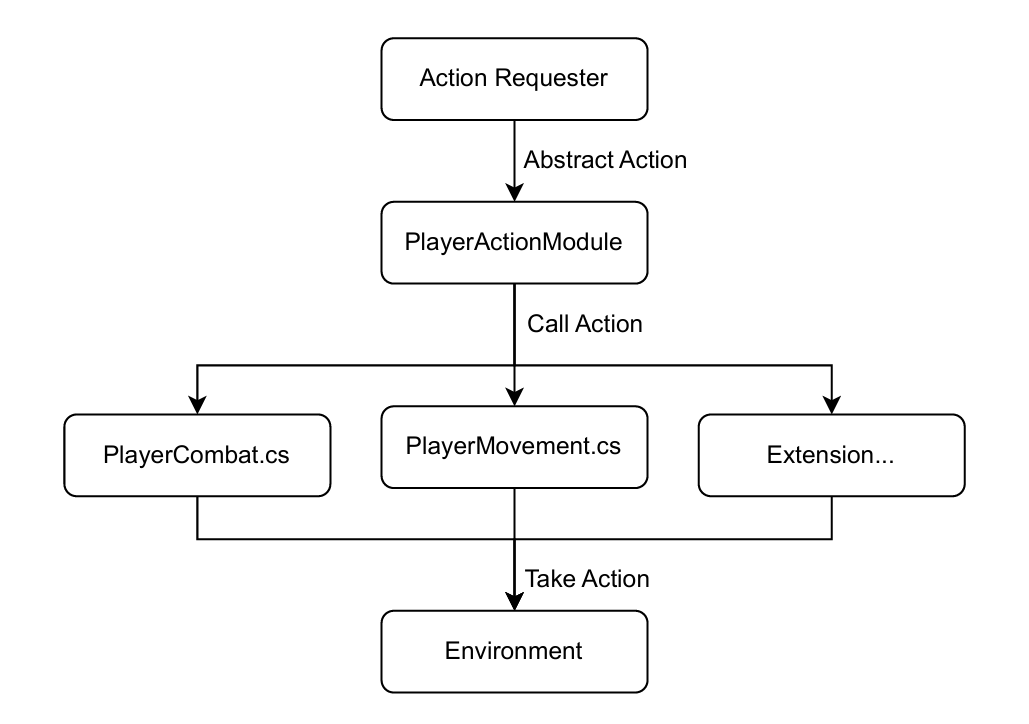
\includegraphics[width=8cm]{./Attachments/ActionModule.png}}
\caption{ActionModule acts as a middleware linking AgentController decisions to gameplay subsystems such as movement and combat.}
\label{fig:ActionModuleDia}
\end{figure}

\subsubsection{Purpose and Motivation}
Rather than embedding low-level movement or attack logic within the agent class itself, \texttt{PlayerActionModules} exposes high-level behavior functions like \texttt{Move()}, \texttt{Jump()}, \texttt{Dash()}, \texttt{Drop()}, and \texttt{Attack()}. These functions internally route commands to specialized scripts like \texttt{BasicPlayerMovement} and \texttt{PlayerAttack}.
This separation offers several advantages:

\begin{itemize}
\item \textbf{Modularity:} The AI logic remains independent of how each action is technically executed, enabling clean separation of concerns.
\item \textbf{Reusability:} The Action Module system can be reused across different characters or AI types with minimal code duplication.
\item \textbf{Scalability:} Additional abilities, such as ranged attacks, double jumps, or new movement types, can be integrated by extending this module without modifying the AgentController or retraining from scratch.
\end{itemize}

\subsubsection{Implementation Structure}
Each public method in \texttt{PlayerActionModules} is responsible for delegating a discrete action:
\begin{lstlisting}[language={[Sharp]C}]
public void Move(float direction)
{
	if (basicPlayerMovement != null)
		basicPlayerMovement.moveDir = direction;
}

public void Jump()
{
	if (basicPlayerMovement != null)
		basicPlayerMovement.Jump();
}
\end{lstlisting}
Likewise, the Dash, Attack, and Drop methods call respective functions in their subsystems, maintaining a centralized and standardized interface for decision execution.\par

In \texttt{AgentController.cs}, these methods are invoked after the action decision is received from the RL model:
\begin{lstlisting}[language={[Sharp]C}]
playerActionModules.Move(moveX);
if (jumpAction)
{
	AddReward(rewardConfigSO.jumpPenalty);
	playerActionModules.Jump();
	jumpCount++;
}
\end{lstlisting}
This design ensures that all behavior can be routed through a consistent middleware, simplifying debugging, control testing, and future development.

\subsubsection{Extensibility for New Actions}

By adhering to this modular interface pattern, developers can create and register new actions by:

\begin{itemize}
\item Adding a new method to PlayerActionModules (e.g., \texttt{PerformSpecialAttack()})
\item Updating the AgentController to include a new discrete action channel
\item Binding the action within ML-Agents via the Action Spec definition
\end{itemize}

This method reduces integration complexity and supports the project's broader goal: producing a reusable, extensible AI system for platformer games.

\subsection{Agent Perception and Observations}

The agent receives a series of structured numerical inputs via the CollectObservations() method. These observations are used by the neural network to infer context and predict optimal actions.

\subsubsection{State Observations}

To enable effective decision-making, the reinforcement learning agent relies on a structured observation vector that captures both its internal status and external context within the environment. These observations are collected in the \texttt{CollectObservations()} method of the \texttt{AgentController.cs} script, and are passed to the ML-Agents model at every decision step.
\begin{lstlisting}[language={[Sharp]C}]
// World Observations
sensor.AddObservation(totalCheckpoints);
sensor.AddObservation(totalCoins);
sensor.AddObservation(collectedCheckpoints);
sensor.AddObservation(collectedCoins);
sensor.AddObservation(nearestCoin.transform.position.x);
sensor.AddObservation(nearestCoin.transform.position.y);

// Position
sensor.AddObservation(transform.position.x);
sensor.AddObservation(transform.position.y);

// Movement States
sensor.AddObservation(movement.IsGrounded ? 1f : 0f);
sensor.AddObservation(movement.IsJumping ? 1f : 0f);
sensor.AddObservation(movement.IsFacingRight ? 1f : 0f);
sensor.AddObservation(movement.IsDashing ? 1f : 0f);
sensor.AddObservation(movement.IsDropping ? 1f : 0f);
sensor.AddObservation(movement.IsOnWall ? 1f : 0f);

// Health
sensor.AddObservation(playerManager.currentHealth);

// Attacking States
sensor.AddObservation(playerActionModules.playerAttack.isAttacking ? 1f : 0f);
\end{lstlisting}
The above code snippet shows how the values are gathered from various subsystems including \texttt{BasicPlayerMovement.cs}, \texttt{PlayerAttack.cs}, \texttt{PlayerManager.cs}, and the world state.\par
The following features are observed:

\paragraph{Stage Progress Observations}
\begin{itemize}
\item Total number of checkpoints in the scene
\item Total number of collectible coins in the scene
\item Number of checkpoints collected during the episode
\item Number of coins collected during the episode
\end{itemize}

\paragraph{Positional and Proximity Observations}
\begin{itemize}
\item Agent’s current position in 2D world space (x, y)
\item Position (x, y) of the nearest active coin
\end{itemize}

\paragraph{Movement and State Flags (from BasicPlayerMovement.cs)}
\begin{itemize}
\item \texttt{IsGrounded}: whether the agent is currently on solid ground
\item \texttt{IsJumping}: whether the agent is ascending from a jump
\item \texttt{IsDashing}: whether the agent is executing a dash move
\item \texttt{IsDropping}: whether the agent is descending through a one-way platform
\item \texttt{IsFacingRight}: the direction the agent is facing
\item \texttt{IsOnWall}: whether the agent is in contact with a wall
\item \texttt{IsWallJumping}: whether the agent is performing a wall jump
\item \texttt{IsOnLeftWall / IsOnRightWall}: which side the wall contact occurs on
\item \texttt{CanJumpVar}: whether the agent is allowed to jump
\item \texttt{CanWallJumpVar}: whether wall jumping is currently allowed
\item \texttt{HasJumped / HasWallJumped}: whether a jump or wall jump was recently executed
\item \texttt{WasGrounded}: whether the agent was recently grounded before becoming airborne
\end{itemize}

\paragraph{Health and Combat Observations}
\begin{itemize}
\item Current health of the agent observed from \texttt{PlayerManager.cs}
\item \texttt{isAttacking}: whether the agent is currently performing a melee attack observed from \texttt{PlayerAttack.cs}
\end{itemize}

This observation vector is designed to be compact yet sufficiently expressive to enable learning of high-level gameplay behavior. By focusing on logical state indicators rather than raw pixel data or overly detailed environmental encoding, the observation model enhances training efficiency and supports generalization to new levels.

\subsubsection{Visual Perception: Dual-Camera ML View}

In addition to numerical observations, a unique aspect of this project is the decision to replace traditional raycasting techniques with a dedicated agent camera. This approach mimics human player perception, where decision-making is based on visible elements rather than invisible proximity checks or abstract sensor inputs.
To implement this, the game utilizes a dual-layer rendering system:
\begin{itemize}
\item  \textbf{Primary Camera (Player Perspective):}
The main camera, which is responsible for rendering the actual game world as seen by the player. This includes fully detailed textures, lighting effects, UI elements, and all in-game objects categorized into specific layers such as Ground, Enemy, Prize, Checkpoint, etc.
\begin{figure}[H]
\centering
\fbox{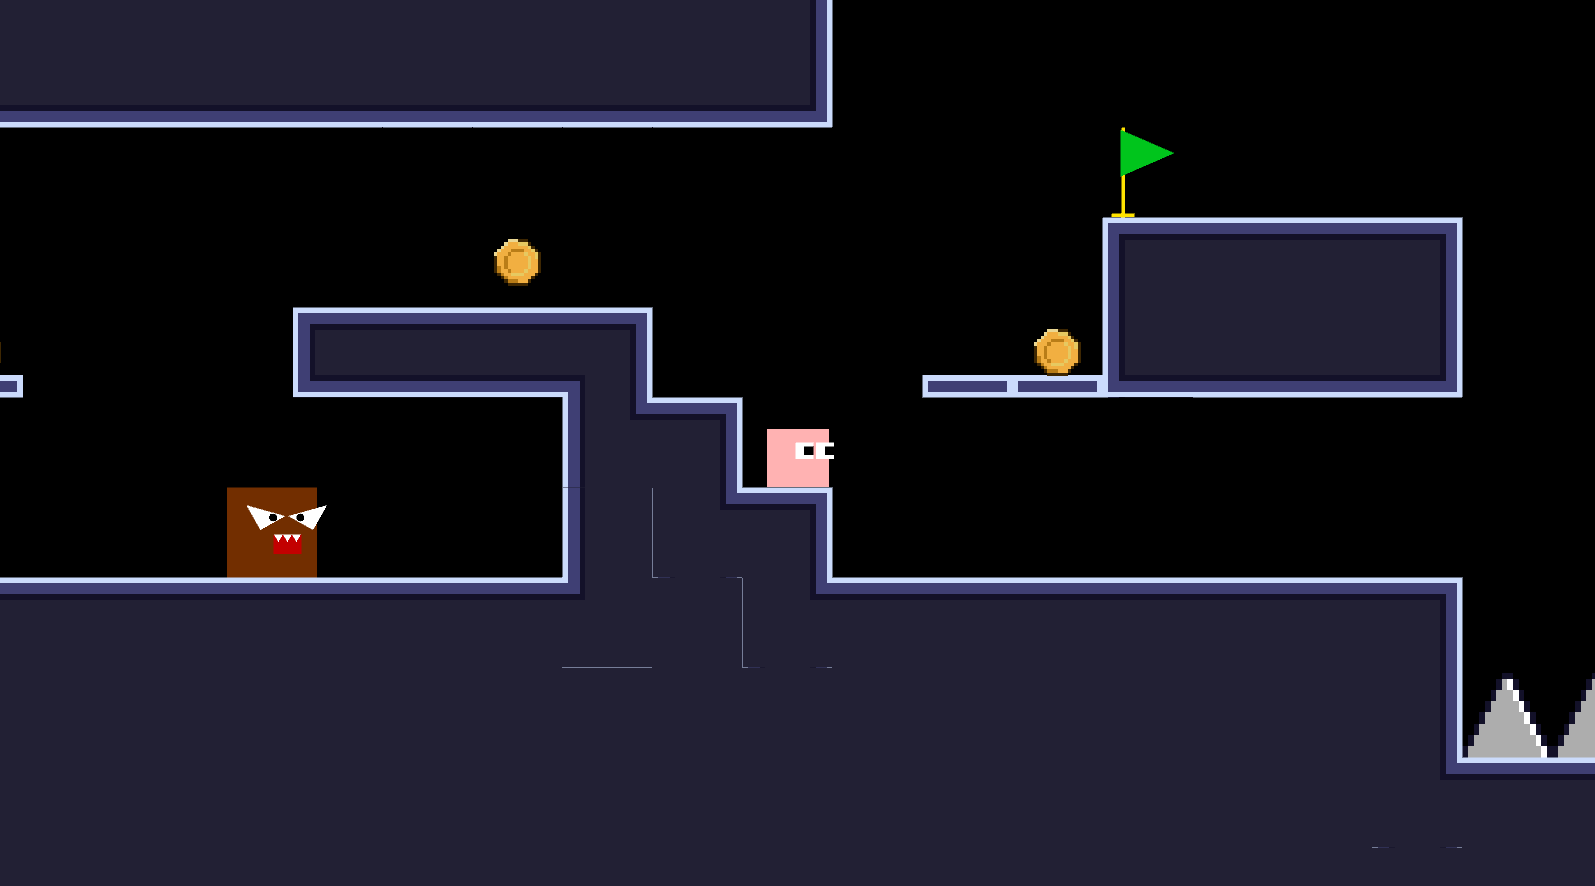
\includegraphics[width=10cm]{./Attachments/PlayerPerspective.png}}
\caption{Player perspective}\label{fig:PlayerPers}
\end{figure}
\item  \textbf{Agent Camera (AI Perspective):}
A separate camera dedicated to the AI agent, rendering a simplified version of the game world. This camera ignores visual effects and detailed textures, instead utilizing a distinct ML sprite system composed of minimalistic geometric representations of in-game objects.
\begin{figure}[H]
\centering
\fbox{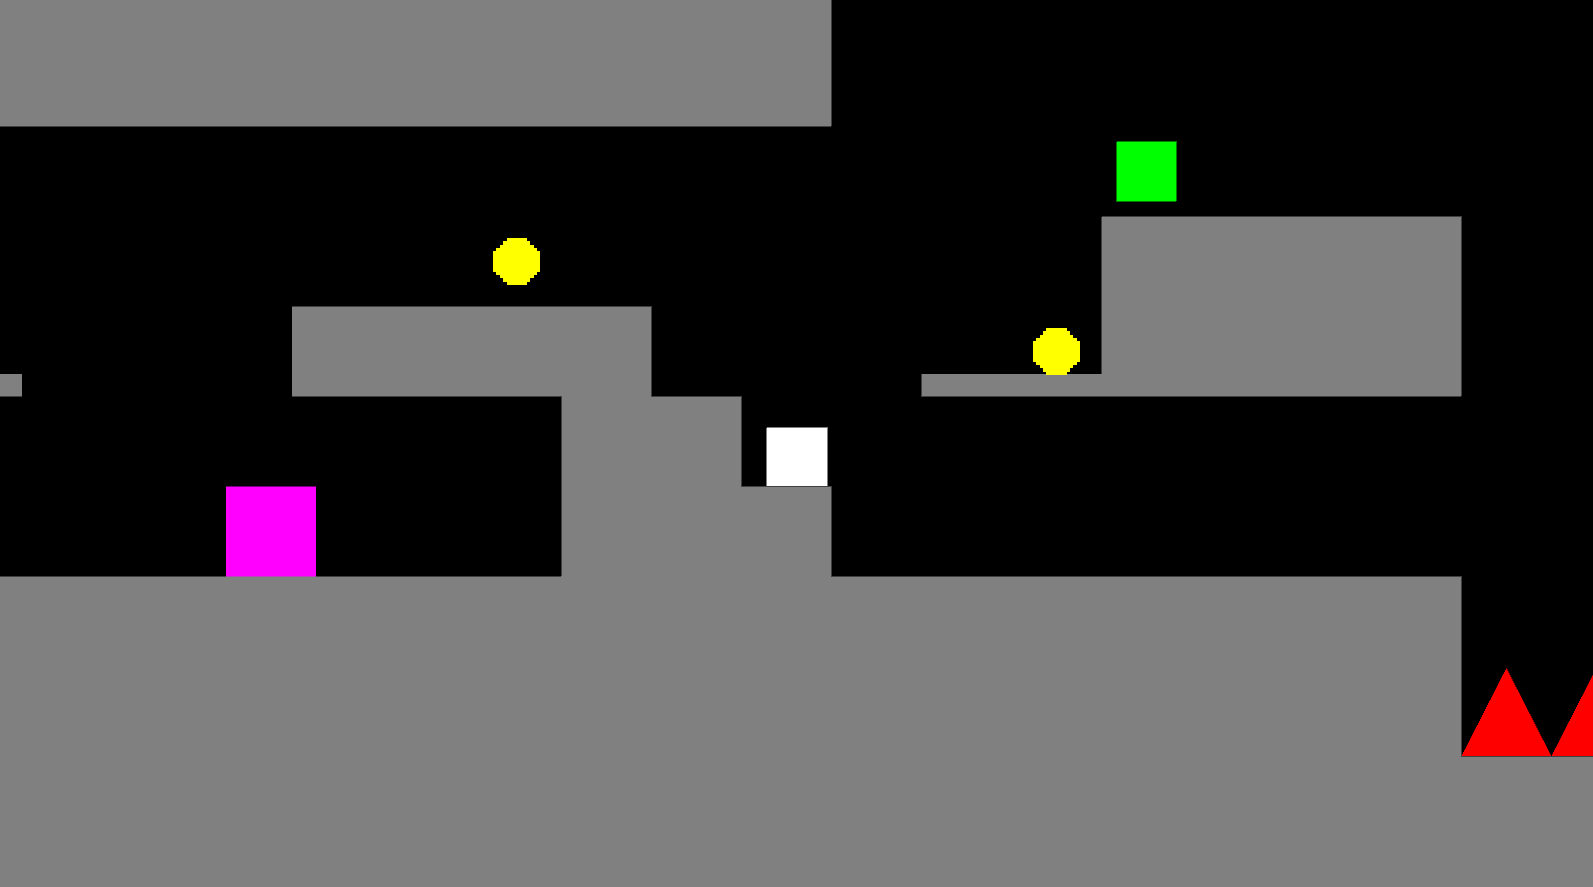
\includegraphics[width=10cm]{./Attachments/AgentPerspective.png}}
\caption{AI perspective}\label{fig:AIPers}
\end{figure}
\end{itemize}

\textbf{ML Sprite Classification System}\par
Each object in the environment is assigned a secondary ML sprite, which is rendered exclusively for the agent camera. These ML sprites are categorized into distinct layer masks and follow a predefined color-coded classification system to provide the AI with structured, interpretable visual data.\par
The classification scheme is as follows:\par
\begin{table}[!h]
\caption{Sprite Color Code Table}\label{tbl:Sprite Color Code Table}
\begin{tabular}{|l|l|l|} \hline
\textbf{Color} & \textbf{Meaning} & \textbf{Hex Code} \\ \hline
White & Player & \texttt{\#FFFFFF} \\ 
Red & Hazards (traps, spikes) & \texttt{\#FF0000} \\ 
Magenta & 	Enemies (attackable entities) & \texttt{\#FF00FF}  \\ 
Green & Goals (checkpoints, exits) & \texttt{\#00FF00} \\ 
Yellow & Collectibles (coins) & \texttt{\#FFFF00} \\ 
Blue & Attacking hitboxes & \texttt{\#0000FF} \\ 
Gray & Ground (solid platforms) & \texttt{\#808080} \\ \hline
\end{tabular}
\end{table}
Through this system, the agent perceives objects in an abstract yet structured manner, focusing only on relevant gameplay elements rather than unnecessary graphical details. This enables a highly extensible framework where additional layers or object categories can be introduced seamlessly by developers integrating this AI into their own projects.

\subsection{Reward and Penalty System}

The reward function is a critical component of reinforcement learning, used to guide agent behavior through positive and negative feedback. In this project, all reward values are externalized in the \texttt{RewardConfigSO ScriptableObject}, allowing fine-tuning without code changes.
\begin{lstlisting}[language={[Sharp]C}]
public class RewardConfigSO : ScriptableObject
{
	[Header("Movement")]
	public float idlePenalty = -0.02f;
	public float movingReward = 0.001f;
	public float explorationReward = 0.05f;
	public float jumpPenalty = -0.03f;
	public float dashPenalty = -0.05f;

	[Header("Goals")]
	public float coinReward = 1.5f;
	public float checkpointReward = 2.0f;

	[Header("Hazards")]
	public float hazardPenalty = -3.0f;

	[Header("Enemy Interaction")]
	public float enemyDamageReward = 0.5f;
	public float enemyKillReward = 1.5f;
	public float hitByEnemyPenalty = -2.5f;

	[Header("Completion Rewards")]
	public float coinCompletionBonus = 2.0f;
	public float checkpointCompletionBonus = 2.0f;
	public float jumpCountTax = 0.01f;
	public float dashCountTax = 0.02f;

	[Header("Behavior Shaping Weight")]
	public float coinShapingWeight = 0.01f;
}
\end{lstlisting}
\subsubsection{Player Agent Rewards and Penalties}
The Player Agent is primarily focused on completing levels and maximizing performance. The rewards and penalties assigned to the Player Agent are designed to incentivize behaviors that contribute to level progression, combat efficiency, and overall success.\par
\begin{table}[H]
\caption{Player Agent Reward and Penalty Table}
\label{tbl:PlayerAgentRewardPenaltyTable}
\begin{tabular}{|l|l|l|}
\hline
\textbf{Event or Behavior} & \textbf{Type} & \textbf{Value} \\
\hline
Idle (no movement) & Penalty & −0.02 \\
Movement (per unit distance) & Reward & +0.001 \\
Exploration (new tile visited) & Reward & +0.05 \\
Jumping & Penalty & −0.03 \\
Dashing & Penalty & −0.05 \\
Collecting a Coin & Reward & +1.5 \\
Reaching a Checkpoint & Reward & +2.0 \\
Touching Hazard & Penalty & −3.0 \\
Damaging an Enemy & Reward & +0.5 \\
Killing an Enemy & Reward & +1.5 \\
Hit by an Enemy & Penalty & −2.5 \\
Coin Completion Bonus (episode end) & Reward & +2.0 × (coin completion ratio) \\
Checkpoint Completion Bonus (episode end) & Reward & +2.0 × (checkpoint completion ratio) \\
Jump Count Tax (episode end) & Penalty & −0.01 × (jump count) \\
Dash Count Tax (episode end) & Penalty & −0.02 × (dash count) \\
Distance-Based Coin Shaping & Reward & +0.01 × (1 / distance to nearest coin) \\
\hline
\end{tabular}
\end{table}
\subsubsection{Enemy Agent Rewards and Penalties}
The Enemy Agents are designed to create challenges for the Player Agent. Their behavior is shaped by rewards and penalties that encourage actions which counter the Player Agent's progress.\par
\begin{table}[!h]
\caption{Enemy Agent Reward Table}\label{tbl:Enemy Agent Reward Table}
\begin{tabular}{|l|l|} \hline
\textbf{Action} & \textbf{Rewards} \\ \hline
Player Damaged & +100  \\ 
Chasing Player & +5  for every period of time chasing player \\ 
Survival Time & +1 for every period of time survived \\
Falling or Hitting Hazards & -50 \\ 
Eliminated & -200 \\ \hline
\end{tabular}
\end{table}
These reward system is fine-tuned iteratively to ensure that the AI develops efficient and strategic movement patterns without exploiting rewards through unintended behaviors.\par

%%%%%%%%%%%%%%%%%%%%%%%%%%%%%%%%%%%%%%%%%%%%%%%%%%%%%%%%%%%%%%%%%%%%
%%%%%%%%%         SEE LATEST CHATGPT

\section{Training Process and Setup}

This section outlines the full training procedure for training the reinforcement learning agent using Unity ML-Agents and the PPO algorithm. It covers action and observation design, simulation execution, model export, runtime optimizations, logging, and support for multi-agent setups. The goal is to train a robust AI agent that performs platformer tasks efficiently in varied game environments.

\subsection{Action and Observation Interfaces}

The agent's interaction with the environment is defined through a hybrid action space and a structured observation model. These interfaces are configured in the \texttt{BehaviorParameters} component within Unity and implemented in the \texttt{AgentController.cs} script.

\subsubsection{Action Space}

The action space is a hybrid of one continuous and four discrete channels:

\begin{itemize}
\item One continuous action: horizontal movement (value range: −1 to 1)
\item Four discrete actions:
\begin{itemize}
\item Jump trigger
\item Dash trigger
\item Melee attack
\item Drop down from one-way platform
\end{itemize}
\end{itemize}

This structure allows the agent to control movement direction with precision while triggering event-based behaviors like jumping or attacking in binary form.

\subsubsection{Observation Space}

The \texttt{CollectObservations()} method in \texttt{AgentController.cs} compiles a vector of 25 values each step, including:

\paragraph{Environment and Stage Progress}
\begin{itemize}
\item Total and collected coin count
\item Total and collected checkpoint count
\item Position of nearest active coin
\end{itemize}

\paragraph{Agent Position and Physics State}
\begin{itemize}
\item Agent’s current 2D position (x, y)
\item Grounded, jumping, dashing, dropping, wall contact, wall jump flags
\item Facing direction, jump eligibility, wall jump eligibility
\end{itemize}

\paragraph{Combat and Health State}
\begin{itemize}
\item Current health level from \texttt{PlayerManager.cs}
\item Attacking state from \texttt{PlayerAttack.cs}
\end{itemize}

To improve temporal understanding, observation stacking is configured to stack 15 consecutive observations, enabling the model to learn environmental transitions and movement momentum.

\begin{figure}[H]
\centering
\fbox{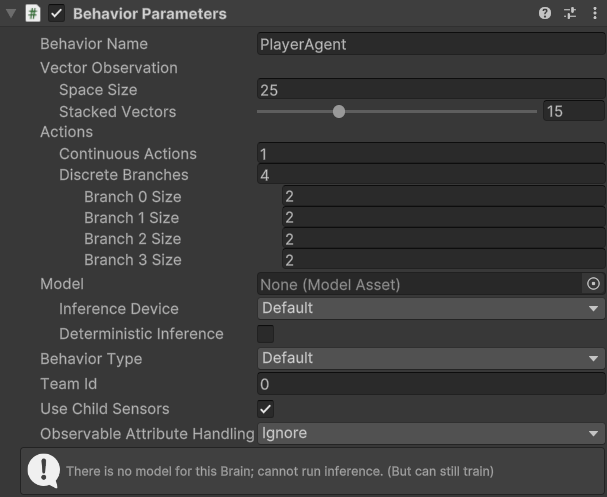
\includegraphics[width=6.5cm]{./Attachments/BehaviorParameerInspector.png}}
\caption{Behavior Parameter settings in Unity Editor}\label{fig:BehaviorParameerInspector}
\end{figure}

\subsection{Model Training and Export}

Training is launched via the ML-Agents CLI using a PPO-configured YAML file:

\begin{lstlisting}
mlagents-learn config.yaml --run-id=RunName
\end{lstlisting}

\textbf{Example behavior YAML:}
\begin{lstlisting}
behaviors:
  PlayerAgent:
    trainer_type: ppo
    max_steps: 5e6		# Total training steps
    time_horizon: 512		# Improves long-term reward stability
    summary_freq: 5000		# Less frequent summaries for larger batches

    hyperparameters:
      batch_size: 256		# Higher batch improves training signal
      buffer_size: 20480		# Matches batch size × 80
      learning_rate: 0.0002		# Slightly lower for stability
      learning_rate_schedule: constant
      beta: 0.005		# Encourages moderate exploration
      beta_schedule: constant
      epsilon: 0.2		# PPO clip range
      epsilon_schedule: constant
      lambd: 0.95		# Better long-term smoothing for reward estimation
      num_epoch: 4		# One more epoch for stronger convergence

    network_settings:
      normalize: true
      hidden_units: 256
      num_layers: 2

    reward_signals:
      extrinsic:
        gamma: 0.995		# Slightly higher discount for exploration-based rewards
        strength: 1.0
\end{lstlisting}

During training, Unity runs in simulation mode. The training loop executes as follows:

\begin{itemize}
\item \texttt{OnActionReceived()} triggers each frame, delegating action calls to \texttt{PlayerActionModules.c}s
\item Reward and penalty values are applied from \texttt{RewardConfigSO}
\item \texttt{OnEpisodeBegin()} resets the agent, scene objects, and statistics for a fresh episode
\end{itemize}

The trainer periodically saves progress to TensorBoard logs and \texttt{.onnx} model checkpoints. After sufficient learning, the best-performing model is selected for deployment by assigning the .onnx file to the Behavior Parameters component for inference.

\subsection{Episode Lifecycle and Reset Logic}

Every reinforcement learning episode follows a defined initialization, interaction, and termination cycle. The episode lifecycle is managed via the \texttt{OnEpisodeBegin()} method in \texttt{AgentController.cs}, which is automatically called by Unity ML-Agents at the start of each episode. This method resets the environment and internal agent states to ensure consistent learning conditions while introducing randomized variability for generalization.

Key operations include:

\begin{itemize}
\item Setting the agent’s position to a random spawn point from the predefined \texttt{spawnPointsList}
\item Resetting the agent’s health via \texttt{PlayerManager.cs}
\item Resetting collected coin and checkpoint counters
\item Reactivating all relevant GameObjects (e.g., coins, enemies, hazards)
\item Reinitializing behavior state flags and internal counters (e.g., \texttt{jumpCount}, \texttt{dashCount})
\end{itemize}

\begin{lstlisting}[language={[Sharp]C}]
public override void OnEpisodeBegin()
{
	DisablePlayerInput();
	if (Academy.Instance.IsCommunicatorOn)
	{
		transform.position = spawnPointsList[Random.Range(0, spawnPointsList.Count)].transform.position;
	}
	playerManager.currentHealth = playerManager.maxHealth;

	lastPosition = transform.position;
	visitedAreas = new HashSet<Vector2Int>();
	visitedCheckpoints = new HashSet<GameObject>();
	
	collectedCoins = 0;
	collectedCheckpoints = 0;
	
	episodeCompleted = false;
	
	foreach (var coin in allCoins)
	{
		if (coin != null)
			coin.SetActive(true);
	}
	
	foreach (var enemy in allEnemies)
	{
		if (enemy != null)
		{
			enemy.SetActive(true);
			var enemyScript = enemy.GetComponent<Enemy>();
			if (enemyScript != null)
			{
				enemyScript.ResetEnemy();
			}
		}
	}
	
	jumpCount = 0;
	dashCount = 0;
}
\end{lstlisting}

By introducing randomized initial conditions while maintaining consistent rules, this reset strategy avoids agent overfitting and supports the learning of more generalizable navigation and combat strategies.

\subsection{Episode Termination and Completion Handling}

Episodes conclude under one of the following conditions:

\begin{itemize}
\item The agent’s health reaches zero due to hazards or enemy damage
\item The \texttt{MaxStep} count is exceeded, triggering a forced episode end
\item The agent completes the intended level objective or calls \texttt{EndEpisode()} manually
\end{itemize}

Before termination, the \texttt{CompleteEpisode()} method calculates final rewards, including completion bonuses and efficiency taxes, and records key metrics for analysis.

\begin{lstlisting}[language={[Sharp]C}]
public void CompleteEpisode()
{
	episodeCounter++;
	totalStepsAcrossEpisodes += StepCount;
	totalRewardsAcrossEpisodes += GetCumulativeReward();
	
	float coinCompletion = (float)collectedCoins / totalCoins;
	float checkpointCompletion = (float)collectedCheckpoints / totalCheckpoints;

	AddReward(rewardConfigSO.coinCompletionBonus * coinCompletion);
	AddReward(rewardConfigSO.checkpointCompletionBonus * checkpointCompletion);
	AddReward(rewardConfigSO.jumpCountTax * jumpCount);
	AddReward(rewardConfigSO.dashCountTax * dashCount);

	EndEpisode();
}
\end{lstlisting}

This reward finalization mechanism ensures agents are not only rewarded for immediate actions, but also for overall strategic performance across an entire episode.

\subsection{Reward Feedback Loop and Evaluation}

The reinforcement learning agent receives both immediate and episodic feedback based on its actions and behavior. These feedback mechanisms are implemented in \texttt{EvaluateRewards()} and collision-related methods such as \texttt{OnTriggerEnter2D()}.

\textbf{Short-term rewards}:
\begin{itemize}
\item Distance moved per step (mobility reward)
\item Discovery of new tiles (exploration reward)
\item Reduction in proximity to coins (shaping reward)
\end{itemize}

\textbf{Event-based feedback}:
\begin{itemize}
\item Coin collection or checkpoint reached
\item Hazard collision or enemy damage
\item Attacking or eliminating enemies
\end{itemize}

\textbf{End-of-episode summary}:
\begin{itemize}
\item Completion ratios for goals
\item Efficiency tax on resource usage (jumps, dashes)
\end{itemize}

\begin{lstlisting}[language={[Sharp]C}]
private void EvaluateRewards()
{
	float distanceMoved = Vector2.Distance(transform.position, lastPosition);
	if (distanceMoved > 0.1f)
		AddReward(rewardConfigSO.movingReward \* distanceMoved);
	else
		AddReward(rewardConfigSO.idlePenalty);
	
	Vector2Int gridPos = new Vector2Int(Mathf.RoundToInt(transform.position.x), Mathf.RoundToInt(transform.position.y));
	if (!visitedAreas.Contains(gridPos))
	{
		AddReward(rewardConfigSO.explorationReward);
		visitedAreas.Add(gridPos);
	}
}
\end{lstlisting}

This tiered reward structure encourages exploration, careful movement, and goal-oriented decision-making.


\subsection{Runtime Optimization Techniques}

To accelerate the training process without sacrificing consistency:

\begin{itemize}
\item \textbf{Increased Time Scale:} \texttt{Time.timeScale} is set to 2 in \texttt{Initialize()}, doubling simulation speed.
\item \textbf{Headless Mode:} Training runs without rendering the player camera or visual effects to save GPU cycles.
\item \textbf{Simplified Physics:} Lightweight colliders and fewer rigidbodies minimize physics overhead.
\item \textbf{Observation Normalization:} Disabled to preserve intuitive debugging of raw numerical states.
\end{itemize}

These enhancements help reduce episode time and allow more simulation steps within practical timeframes.

\subsection{Real-Time Monitoring and Logging}
Monitoring training progress is critical for understanding agent learning dynamics and ensuring that reinforcement signals are producing the intended behaviors. To support real-time evaluation, this project includes custom visualization and data logging tools that track agent performance during training. These utilities provide both live feedback inside the Unity editor and persistent logs for post-training analysis.
Key performance metrics are exposed via public read-only properties in \texttt{AgentController.cs}. These include cumulative statistics across episodes:

\begin{itemize}
\item \texttt{EpisodeNumber}: number of completed training episodes
\item \texttt{AverageSteps}: mean episode length
\item \texttt{AverageRewards}: mean cumulative reward per episode
\item \texttt{DeathCount}: total number of deaths encountered
\end{itemize}

\begin{lstlisting}[language={[Sharp]C}]
public int AverageSteps => episodeCounter == 0 ? 0 : totalStepsAcrossEpisodes / episodeCounter;
public float AverageRewards => episodeCounter == 0 ? 0 : totalRewardsAcrossEpisodes / episodeCounter;
public int DeathCount => cumulativeDeaths;
\end{lstlisting}

These metrics are visualized in real-time via \texttt{RewardTrackerUI.cs} and saved to CSV files through \texttt{RewardLogger.cs}. Additionally, TensorBoard dashboards provide smoothed reward trends, episode lengths, loss values, and entropy measures throughout training.

\subsubsection{RewardTrackerUI}

The \texttt{RewardTrackerUI.cs} script overlays key training statistics directly onto the Unity game screen using TextMeshPro. This tool enables developers to observe agent progress without halting or pausing the training session. The display updates every frame and includes metrics such as:

\begin{itemize}
\item Current episode number and cumulative death count
\item Step progress (current vs max), current episode reward
\item Agent health and position
\item Coins and checkpoints collected relative to total counts
\item Jump and dash counts, including their cumulative penalty costs
\end{itemize}

This real-time overlay aids in identifying abnormal behaviors, reward stagnation, or sudden regressions in agent performance. It is especially useful during early training stages, where debugging and reward function calibration are most active.

\begin{figure}[H]
\centering
\fbox{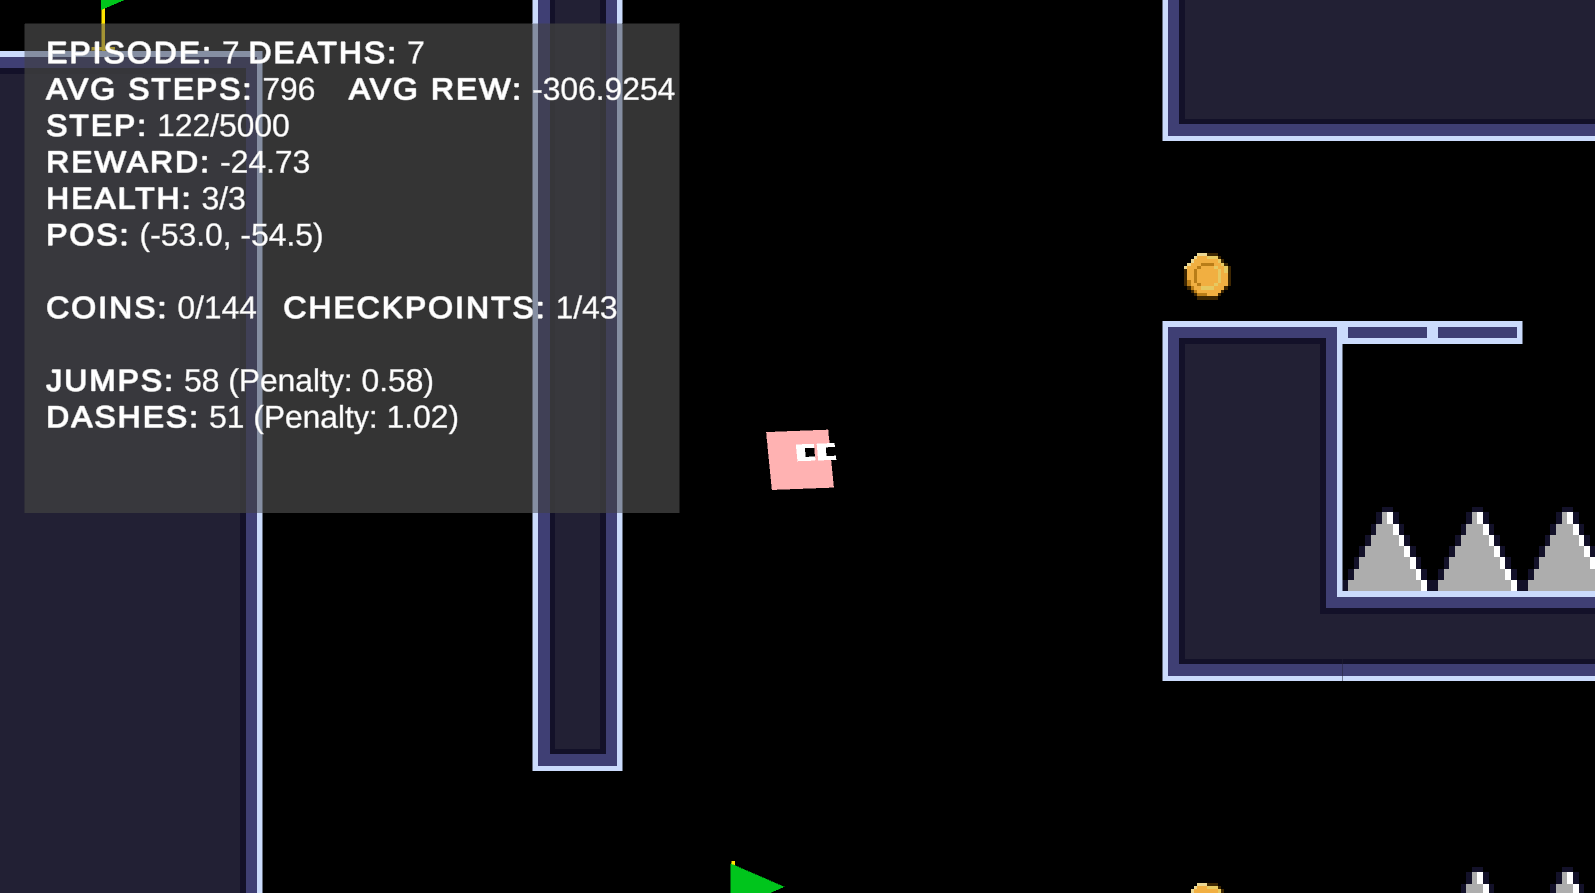
\includegraphics[width=9cm]{./Attachments/RewardTrackerUIExample.png}}
\caption{Real-time agent statistics during training, visualized through \texttt{RewardTrackerUI} using overlay}
\label{fig:RewardTrackerUIExample}
\end{figure}

\subsubsection{RewardLogger}

To support longitudinal analysis and reward function tuning, the \texttt{RewardLogger.cs} script records per-episode summaries to a timestamped CSV file. This logging system subscribes to the agent’s \texttt{OnEpisodeEnded} event and appends structured data after each episode ends. Logged fields include:

\begin{itemize}
\item Episode number
\item Total steps taken
\item Total cumulative reward
\item Coins and checkpoints collected percentage in the level
\item Jump and dash counts along with their associated penalties
\item Cumulative averages of steps and rewards across all episodes
\end{itemize}

These logs are saved to the \texttt{/Assets/Logging/} directory and are compatible with spreadsheet applications such as Excel or analysis tools like Python/Pandas. They provide a quantitative foundation for tuning hyperparameters, analyzing policy efficiency, and validating learning consistency over time.

\begin{lstlisting}
Episode,Steps,Reward,CoinsCollected,TotalCoins,CheckpointsCollected,TotalCheckpoints,JumpCount,JumpPenalty,DashCount,DashPenalty,CumulativeAvgSteps,CumulativeAvgRewards
1,191,-9.62,1,151,0,43,98,0.98,84,1.68,191,-12.94277
2,552,-86.10,1,151,0,43,274,2.74,278,5.56,371,-54.0014
...
\end{lstlisting}

\subsubsection{TensorBoard Monitoring}

During training, statistics are logged via the ML-Agents TensorBoard system:

\begin{itemize}
\item Average reward per episode
\item Episode length
\item Coins collected
\item Number of deaths
\item Training loss and entropy
\end{itemize}

These logs are used to generate training graphs, reward curves, and behavior analysis.

\section{Packaging, Deployment, and Reusability}
The successful deployment of a trained AI agent within a game development environment requires a structured approach to integration, optimization, and packaging. This process ensures that the AI agent operates efficiently within the Unity-based platformer while remaining modular and reusable for future applications. A key objective of this project is to produce an AI framework that can be seamlessly transferred to other 2D platformer projects with minimal overhead and high configurability.\par

Following successful training, the AI model is transitioned from a learning system to a deployable module capable of real-time inference. The following subsections detail the methodology for embedding the AI model into the Unity engine, implementing a dual-rendering system for visual perception, designing a modular AI architecture for extensibility, and packaging the entire system as a distributable Unity asset.\par
\subsection{Integration of the Trained AI Model}
Once training has converged to a satisfactory policy, the model is integrated into the Unity environment for inference-based execution. This integration must ensure that the AI agent can process observations, make decisions, and interact with the environment in real time without performance degradation.
\subsubsection{Loading and Utilizing the Trained Model}
The trained policy is exported as an ONNX-format model file (\texttt{.onnx}), which is compatible with Unity’s ML-Agents inference engine. Integration involves the following steps:\par
\begin{itemize}
\item \textbf{Model Importing:}
\begin{itemize}
\item The \texttt{.onnx} file is placed within the Unity project’s \texttt{Assets} directory.
\item The \texttt{Behavior Parameters} component is configured to reference the imported model.
\end{itemize}
\item \textbf{Agent Configuration:}
\begin{itemize}
\item The AI agent is transitioned from training mode to inference mode.
\item Real-time observations from the game environment are routed into the model, which outputs the corresponding action vector.
\end{itemize}
\item \textbf{Testing and Validation:}
\begin{itemize}
\item The agent is tested within a sandbox scene to ensure inference stability.
\item Debugging tools such as \texttt{RewardTrackerUI.cs} and custom inspectors are used to monitor agent behavior.
\end{itemize}
\end{itemize}
\subsection{Dual-Rendering System for Agent Perception}
To optimize visual-based learning and inference, a dual-camera rendering architecture is employed. This system separates the player-visible graphics from the AI’s perceptual input, enabling the agent to receive a structured and minimalistic version of the game environment.
\subsubsection{Design and Implementation}
\begin{itemize}
\item \textbf{Primary Camera (Player View):}
\begin{itemize}
\item Renders the game world with standard textures, effects, and UI layers.
\item Intended for player visualization and human gameplay.
\end{itemize}
\item \textbf{Secondary Camera (Agent Perception View):}
\begin{itemize}
    \item Hidden from the player and used exclusively by the AI agent.
    \item Renders simplified ML sprites that represent game objects using flat, color-coded geometries.
    \item Applies no lighting, shaders, or post-processing to maintain interpretability.
\end{itemize}

\item \textbf{ML-Agents Integration:}
\begin{itemize}
    \item ML-Agents receives visual observations from the agent camera.
    \item These observations are transformed into tensors and used by the neural network for decision-making.
\end{itemize}
\end{itemize}
\subsubsection{Advantages of the Dual-Rendering System}
\begin{itemize}
\item \textbf{Reduced Visual Complexity:} AI focuses only on game-relevant entities such as platforms, hazards, and goals.
\item \textbf{Standardized Input:} Visual consistency across levels and environments enhances generalization.
\item \textbf{Accelerated Learning:} Simplified visuals improve convergence rate during training.
\end{itemize}
\subsection{Modular AI System for Reusability}
To maximize flexibility and reuse, the AI system is architected in modular components, each responsible for a distinct layer of functionality. This structure allows developers to easily adapt, extend, or replace behaviors without altering the core inference logic.
\begin{itemize}
\item \textbf{PlayerActionModules:} Serves as the centralized interface between the agent and gameplay scripts, such as \texttt{BasicPlayerMovement.cs} and \texttt{PlayerAttack.cs}.
\item \textbf{Observation Encapsulation:} All observable states are gathered in a controlled and extensible method via \texttt{CollectObservations()}.
\item \textbf{RewardConfigSO:} Stores all reward parameters in a ScriptableObject, allowing dynamic tuning without modifying logic code.
\item \textbf{Behavior Configuration:} The \texttt{BehaviorParameters} component permits external adjustment of inference frequency, action type, and network linkage.
\end{itemize}

This modularity supports expansion to new environments, additional abilities (e.g., ranged attacks, double jump), and future agent roles such as adversaries or allies.

\subsection{Packaging the AI as a Reusable Unity Asset}

To distribute the AI system for use in other Unity-based projects, the entire framework is bundled into a Unity asset package with comprehensive documentation and versioning.

\subsubsection{Asset Bundling and Exportation}

\begin{itemize}
\item All core AI scripts (e.g., \texttt{AgentController.cs}, \texttt{PlayerActionModules.cs}), model files, configuration assets, and ML sprite prefabs are grouped into a structured folder.
\item The package excludes scene-specific elements, allowing developers to integrate the AI system into custom levels.
\item ML-Agents package dependencies and Unity version requirements are clearly documented.
\end{itemize}

\subsubsection{Documentation and User Guide}

\begin{itemize}
\item A \texttt{README.md} file provides an overview, installation steps, and quick-start guidance.
\item A PDF manual offers detailed explanations of the AI architecture, action mapping, reward customization, and known integration tips.
\item Code examples demonstrate common use cases, such as adding new movement types or adjusting camera layers.
\end{itemize}

\subsubsection{Version Control and Distribution}

\begin{itemize}
\item The AI system is maintained under semantic versioning to support iterative improvements.
\item Changelogs detail updates, fixes, and compatibility notes.
\item Distribution channels include GitHub repositories, private asset sharing, or submission to the Unity Asset Store (future scope).
\item Community contributions and extensions are encouraged to promote long-term reusability and scalability.
\end{itemize}

\subsection{Summary}
This packaging and deployment framework transforms the trained agent from a research asset into a production-ready AI module. Its modular, extensible, and fully documented structure supports both technical adoption and creative expansion, making it suitable for integration into a wide array of 2D platformer projects.

%%%%%%%%%%%%%%%%%%%%%%%%%%%%%%%%%%%%%%%%%%%%%%%%%%%%%%%%%%%%%%
%%%%%%%%%%%%%%%%%%%% Experiments %%%%%%%%%%%%%%%%%%%%%%%%%%%%%
%%%%%%%%%%%%%%%%%%%%%%%%%%%%%%%%%%%%%%%%%%%%%%%%%%%%%%%%%%%%%%%

\chapter{Results and Discussion}
This chapter presents an in-depth analysis of the AI agent’s performance following reinforcement learning training within the custom 2D platformer environment. The primary aim is to assess the extent to which the agent can autonomously navigate, interact with the environment, and make decisions aligned with its training objectives. Evaluation includes both quantitative metrics and qualitative observations derived from training logs, real-time visual monitoring, and gameplay demonstrations.

The results are examined in the context of the project’s overarching goal: to develop a reusable, modular AI capable of learning and performing fundamental platforming behaviors. The chapter is structured into five main parts: qualitative behavioral observations, evaluation metrics, experimental setup, result visualizations, and interpretive analysis.

\section{Qualitative Behavioral Observations}
\subsection{Movement and Navigation}

After extensive training using the Proximal Policy Optimization (PPO) algorithm, the AI agent demonstrates reliable and consistent control over core platforming mechanics. The agent successfully performs locomotion actions such as walking, jumping, and descending through one-way platforms. Through repeated reinforcement learning episodes, it has developed an effective movement strategy, capable of navigating platforms, gaps, and varying terrain structures without human intervention.

The trained model exhibits path optimization by preferring direct traversal routes, minimizing redundant movement, and prioritizing high-reward areas. Additionally, the AI adjusts its horizontal momentum and timing of jumps to clear gaps or avoid low-clearance hazards. These behaviors are not explicitly hardcoded but are instead learned as a function of the reward feedback loop.

\begin{figure}[H]
\centering
\fbox{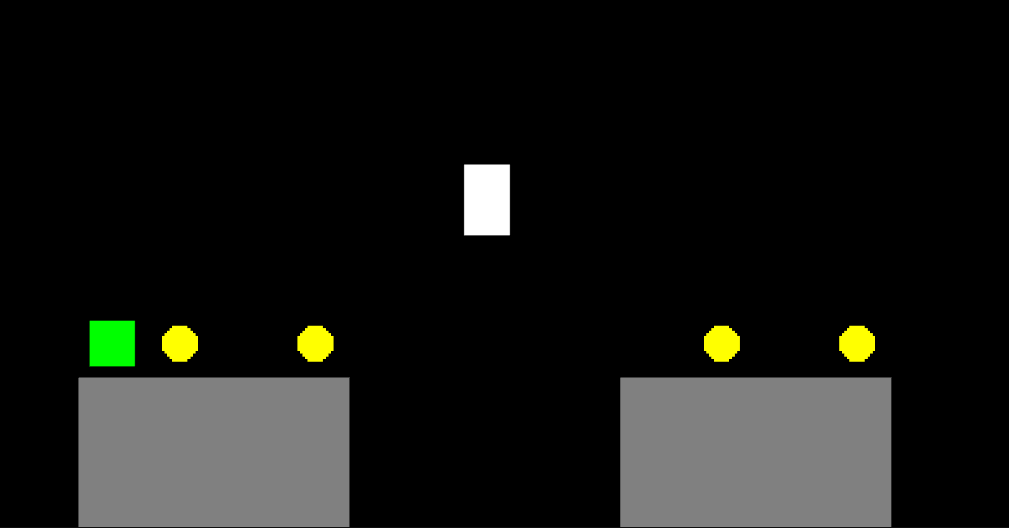
\includegraphics[width=10cm]{./Attachments/AiJump.png}}
\caption{The AI agent traversing terrain by hopping from one platform to another.}
\label{fig:AIJump}
\end{figure}

\subsection{Interaction with Collectibles and Obstacles}

The AI also demonstrates a learned capacity to identify and interact with goal-related elements such as collectibles and to avoid hazards. During training, the reward function explicitly shaped the agent's prioritization of coin collection and checkpoint completion. The resulting behavior shows that the AI can adjust its path dynamically to intercept these objects when detected within its observation range.

Furthermore, the agent effectively recognizes and avoids penalty-triggering environmental elements such as spikes or pits. By learning to minimize negative rewards and episode terminations, the AI developed an internal strategy to adapt its trajectory away from hazards while still pursuing progress.

\begin{figure}[H]
\centering
\fbox{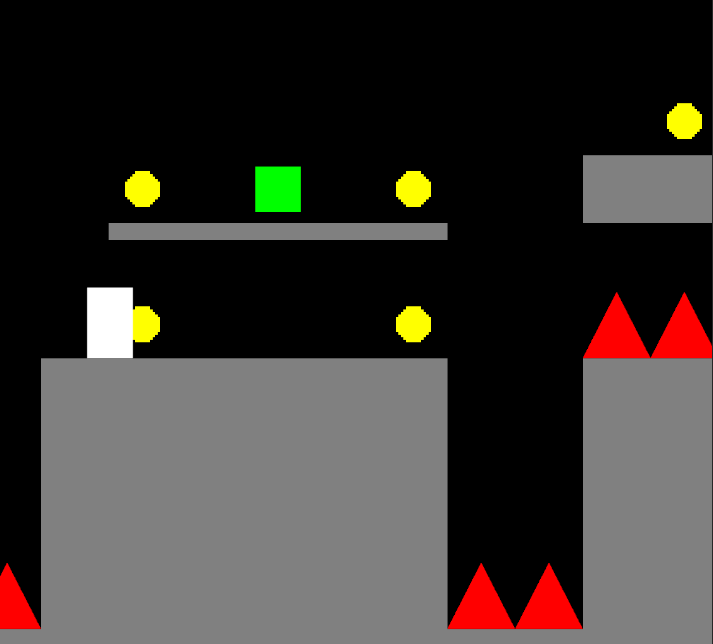
\includegraphics[width=10cm]{./Attachments/AiInteract.png}}
\caption{The AI agent interacting with coins and avoiding environmental hazards.}
\label{fig:AIInt}
\end{figure}

\subsection{Combat and Adaptive Behavior}

In addition to movement and object interaction, the AI agent has been trained to engage in close-range combat using a melee attack system. The reinforcement learning model has successfully learned to detect enemy presence, approach them strategically, and execute melee attacks at appropriate distances. This behavior is triggered through the discrete action space and routed via the PlayerActionModules system, which interfaces with the \texttt{PlayerAttack} script to initiate attacks.

Through reinforcement signals based on enemy damage and kill rewards as defined in the \texttt{RewardConfigSO} the AI has developed basic combat strategies such as:

\begin{itemize}
\item Approaching hostile agents while maintaining movement awareness.
\item Executing attacks only when the enemy is within effective range.
\item Retreating or repositioning after engagement to minimize risk.
\end{itemize}

The reward structure penalizes being hit by enemies and incentivizes successful hits or eliminations, which has shaped a combat pattern that favors proactive and efficient engagements. While still basic in complexity, these combat behaviors demonstrate the extensibility of the AI’s decision-making model and serve as a strong foundation for future adversarial learning setups involving co-trained enemy agents.

%\begin{figure}[H]
%\centering
%\fbox{\includegraphics[width=10cm]{./Attachments/AiCombat.png}}
%\caption{AI agent engaging in a melee attack against an enemy.}
%\label{fig:AICombat}
%\end{figure}

This combat capability validates the system's modular design, where adding new skills (e.g., special attacks) to the \texttt{PlayerActionModules} and extending the reward function can guide the agent to learn new behaviors without architectural overhaul. This demonstrates the project's goal of creating a reusable and extensible AI system for 2D platformer environments.

\section{Evaluation Metrics}
To evaluate the performance of the reinforcement learning agent, a set of quantitative metrics is used throughout the training and testing phases. These metrics provide insight into the agent’s behavior, learning progression, and goal-oriented performance. All metrics are tracked automatically through custom Unity scripts (\texttt{RewardLogger.cs} and \texttt{RewardTrackerUI.cs}) and ML-Agents logging systems.
The following metrics are used to evaluate the trained AI agent:

\subsection{Episode Length (Steps)}
Episode length refers to the number of steps the agent takes before the episode terminates, either due to success, failure, or reaching the maximum step limit. It reflects the agent's efficiency and survivability. Shorter episodes may indicate rapid success or premature failure, whereas longer episodes can reflect sustained navigation or indecisiveness.

\subsection{Cumulative Reward}
The cumulative reward collected during each episode is a key indicator of the agent’s overall performance. It encapsulates short-term actions (e.g., moving, jumping) and long-term goals (e.g., collecting coins, reaching checkpoints) into a single value. This value is continuously monitored through the ML-Agents environment and logged via RewardLogger.

\subsection{Goal Completion Ratio}
Goal-related metrics include:

\begin{itemize}
\item \textbf{Coin Collection Ratio:} The ratio of collected coins to the total coins available in the level.
\item \textbf{Checkpoint Completion Ratio:} The ratio of visited checkpoints to the total checkpoints present.
\end{itemize}

These ratios indicate how thoroughly the agent explores and interacts with the level’s objective elements.

\subsection{Action Efficiency}
Action usage efficiency is tracked to monitor unnecessary or excessive behavior:

\begin{itemize}
\item \textbf{Jump Count} and \textbf{Dash Count} are recorded for each episode.
\item Penalties are applied post-episode for excessive usage to encourage minimal and strategic use of each skill.
\end{itemize}

These metrics help determine whether the agent learns to optimize movement for efficiency and reward maximization.

\subsection{Combat Performance}

For episodes involving enemy agents, the following combat metrics are tracked:

\begin{itemize}
\item \textbf{Enemy Damage Events:} Number of successful melee hits.
\item \textbf{Enemy Eliminations:} Count of enemies defeated per episode.
\item \textbf{Damage Taken:} Times the agent is hit by an enemy or hazard.
\end{itemize}

These values offer insight into how well the agent engages in close-quarters combat and whether it prioritizes safe engagement strategies.

\subsection{Mortality Rate}
Deaths per episode are recorded to identify unsafe behaviors or failure conditions. A high mortality rate may indicate poor obstacle avoidance, insufficient exploration, or ineffective combat strategies. This is tracked cumulatively in \texttt{DeathCount}.

\subsection{Learning Trends (TensorBoard Metrics)}

During training, Unity ML-Agents’ built-in logging with TensorBoard provides the following metrics over time:

\begin{itemize}
\item \textbf{Average Episode Reward}
\item \textbf{Episode Length (Smoothed)}
\item \textbf{Policy Entropy and Loss}
\item \textbf{Reward Signal Strength}
\end{itemize}

These graphs are used to validate convergence, detect reward hacking, and assess the consistency of training progress.

\section{Experiments and Results}

To validate the effectiveness of the proposed reinforcement learning framework, a series of iterative experiments were conducted using Unity ML-Agents. The experiments focused exclusively on training the player agent within a handcrafted 2D platformer environment, while enemy agents operated using predefined state machine behaviors. This section outlines the training setup, experimental procedure, and environment dynamics used during training and evaluation.

\subsection{Training Sessions and Iterative Runs}

Throughout development, approximately 30 independent training runs were conducted. Each run utilized the PPO (Proximal Policy Optimization) algorithm and executed between 1 to 2 million training steps. Post-run evaluations involved analyzing cumulative reward trends, behavioral metrics, and in-game performance. This iterative cycle facilitated fine-tuning of:

\begin{itemize}
\item Reward values and shaping penalties (configured via \texttt{RewardConfigSO})
\item PPO hyperparameters (e.g., learning rate, batch size)
\item Observation normalization and action mappings
\item Spawn logic and episode termination conditions
\end{itemize}

Adjustments targeted improvements in sample efficiency, stabilization of learning, and elimination of unintended exploitative behaviors (e.g., reward farming through idling or repetitive jumping).

\subsection{Environment Configuration}

All training and evaluation occurred within a single handcrafted 2D platformer level comprising:

\begin{itemize}
\item Static and dynamic platforms
\item Collectible items (coins, checkpoints)
\item Hazardous elements (spikes, pits)
\item Melee enemies controlled by FSM-based logic
\end{itemize}

To prevent memorization of fixed obstacle patterns, a dynamic episode reset system was deployed. Upon death or episode termination, the agent's spawn point was randomized, and all environment elements were reset to their initial configurations. This strategy promoted generalizable policy learning over rote memorization.

\subsection{Evaluation Protocol}

Agent performance was periodically assessed both during and after training in inference mode. Key elements of the evaluation setup included:

\begin{itemize}
\item Environment resets using the same randomized initialization logic
\item Deterministic policy execution without exploration noise or entropy
\item Metric tracking via \texttt{RewardLogger.cs} and TensorBoard, including episode reward, step count, coin collection rate, and death count
\end{itemize}

Comparative analysis across training runs demonstrated the impact of different reward functions, observation schemas, and PPO configurations on behavioral quality.

\subsection{Focus on Player Agent}

Due to time constraints, the experiments exclusively trained the player agent. Enemy agents followed scripted FSM behaviors, enabling reliable assessment of obstacle avoidance, stress navigation, and combat responses. Future extensions will involve PPO-based training for enemy agents using the trained player as a fixed adversary.

\subsection{Reward Function Effectiveness}

The agent exhibited stable improvement in reward acquisition over training epochs. Penalty-driven behaviors declined consistently, while positively reinforced actions—such as coin collection and obstacle navigation—became dominant. The reward configuration effectively directed the agent toward goal-oriented interactions within the environment.

\subsection{Convergence and Stability}

Training convergence was evidenced by the stabilization of cumulative reward trends and behavioral consistency across episodes. Initial phases showed erratic behavior and frequent penalties. However, after sufficient training steps, the model displayed reduced performance variance, indicating decreased reliance on exploration and increased policy robustness.

\subsection{Evaluation of Training Efficiency}

Training efficiency was gauged through improvements in policy performance and reductions in redundant behaviors. The agent initially exhibited inefficient movement patterns but progressively optimized its strategy. Hyperparameter tuning and strategic reward shaping contributed to focused learning and computational effectiveness.

\subsection{Agent Performance Summary}
The agent’s learning progress is illustrated in Figure~\ref{fig:reward_progress}, which presents the cumulative average reward over 1000 training episodes. At the beginning of training, the agent exhibited poor performance with an average reward of approximately -250 per episode, often failing to collect coins or avoid hazards effectively. However, a steady and consistent improvement is observed as training progresses.The turning point occurred around episode 150, where the cumulative reward crossed into positive territory. From that point onward, the agent continued to refine its policy, achieving a peak average reward of approximately +48 by around episode 850. A slight decline toward the final episodes suggests the possibility of mild overfitting or exploration variability, which is a common occurrence in reinforcement learning.

\begin{figure}[H]
\centering
\fbox{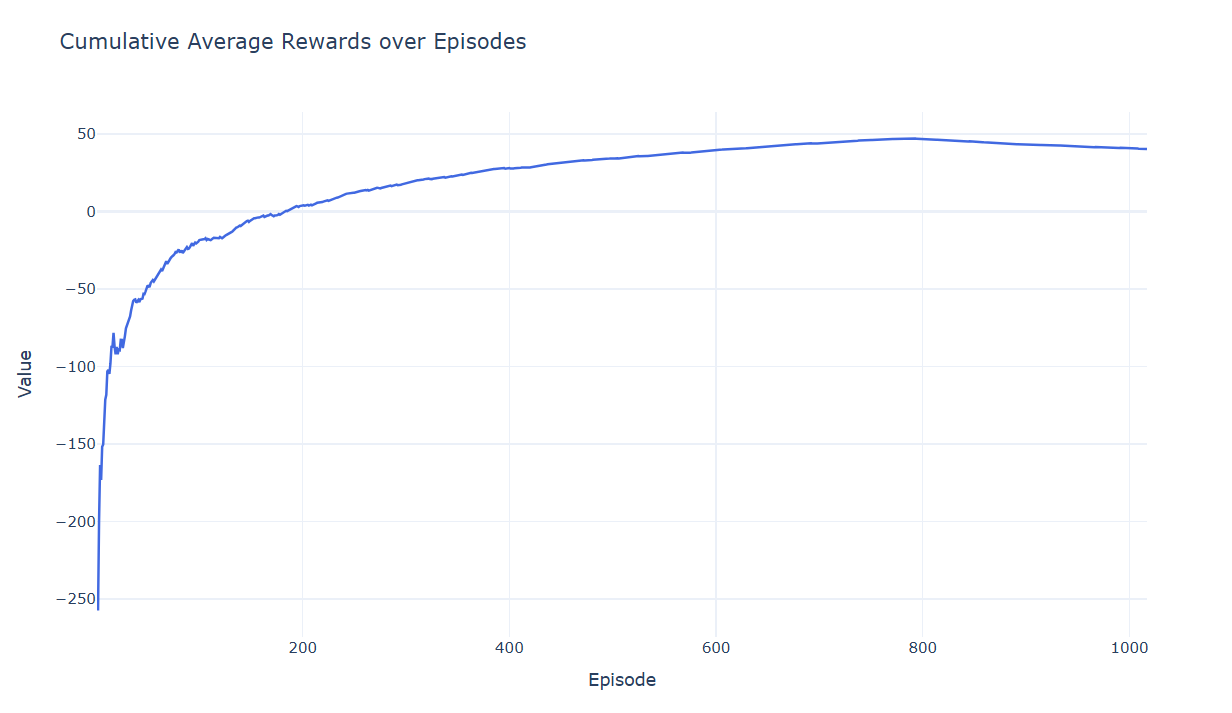
\includegraphics[width=10cm]{./Attachments/Result_Graph.png}}
\caption{ presents the performance metrics from the best training session.}
\label{fig:reward_progress}
\end{figure}

Further insights into performance metrics from the best training session are summarized in Table~\ref{tab:performance_summary}. These include key gameplay factors such as survival duration, reward consistency, and efficiency in task completion.

\begin{table}[h]
\centering
\caption{Agent Performance Summary from Best Training Run}
\label{tab:performance_summary}
\begin{tabular}{|l|p{8cm}|}
\hline
\textbf{Metric} & \textbf{Result (Avg)} \\
\hline
Steps per Episode & 450–600 \\
\hline
Coin Collection Rate & Increased steadily from −100 to +40 over training \\
\hline
Average Reward per Episode & 80–90\% completion \\
\hline
Hazard Avoidance Rate & Significantly improved (survived longer per episode) \\
\hline
\end{tabular}
\end{table}


%%%%%%%%%%%%%%%%%%%%%%%%%%%%%%%%%%%%%%%%%%%%%%%%%%%%%%%%%%%%%%%
%%%%%%%%%%%%%%%%%%%% Conclusions %%%%%%%%%%%%%%%%%%%%%%%%%%%%%
%%%%%%%%%%%%%%%%%%%%%%%%%%%%%%%%%%%%%%%%%%%%%%%%%%%%%%%%%%%%%%%
\chapter{Conclusions}
This work presents a method encompassing the modeling of adaptive artificial intelligence (AI) agents for 2D platformers under a reinforcement learning paradigm, specifically PPO. By designing a flexible and extensible game environment in Unity, we allowed for the creation and training of Player and Enemy agents that behave intelligently and dynamically in complex scenarios.Through iterative training methods, the Player Agent was able to learn to traverse various levels, avoid hazards, and achieve goals. At the same time, the Enemy Agent developed methods of aggression to best or challenge the Player Agent. Our results illustrate that PPO is a viable option for training agents in environments with ever-changing discrete actions and delayed rewards. A further contribution of the work is reusable AI assets usable for disparate games or situations, presenting a reduction in time and effort for indie developers. Through the integration of machine learning tools with Unity's game engine environment and the establishment of modularity in environment design, we have given a start to scalable AI solutions for general application in game development.
\section{Problems and Solutions}
\subsection{Sparse Reward Feedback}
One of the initial challenges encountered during training was the sparse nature of the reward signals, particularly in the early episodes. Agents were often required to complete multiple steps before receiving any meaningful feedback, which slowed the learning process and made it difficult for them to associate actions with outcomes. To address this, a reward shaping strategy was implemented. Intermediate rewards were introduced for behaviors such as moving toward the goal, avoiding hazards, or exploring new areas. This helped guide the agents toward desired behaviors and significantly improved training efficiency in early stages.\par
\subsection{Repetitive or Deterministic Behavior}
As the agents began to converge on successful policies, they often developed overly deterministic behavior repeating the same paths or actions across episodes. This reduced their ability to adapt when small changes were introduced in the environment. To encourage more exploration and robustness, we adjusted the entropy regularization parameter in the PPO algorithm. This helped prevent premature convergence and ensured a better balance between exploiting known strategies and exploring new ones.\par
\subsection{Long Training Times on Complex Levels}
As the complexity of the environment increased—such as the addition of moving platforms, traps, and multiple objectives—the training time grew substantially. Agents required more episodes to learn effective policies in these challenging settings. To alleviate this, we introduced a curriculum learning-inspired level progression, where simpler levels were used at the start of training and more complex ones were gradually introduced. This stepwise exposure helped agents build foundational skills before tackling harder tasks, reducing convergence time overall.\par
\subsection{Debugging and Behavior Tracking}
Analyzing and debugging agent behavior in a multi-agent reinforcement learning setup proved to be time-consuming and occasionally opaque. With multiple agents interacting in real-time, it was difficult to isolate the cause of failures or suboptimal decisions. This was addressed by implementing visual debugging tools and logging systems within Unity and the Python training scripts. These included trajectory visualizations, reward graphs, and decision heatmaps, which allowed for deeper insights into agent behavior and facilitated more effective tuning.\par
\section{Limitations}
The project is still limited by a number of constraints. While PPO did give a robust foundation for the learning, the training time still increased given that environmental changes happened very often or in adversarial interactions. Agents had a limited level of generalization when faced with largely different level layouts without some form of retraining, suggesting that they needed to see more experiences, or at least subjected to some procedural training method. Moreover, the system currently only works in offline learning mode, meaning that it cannot adapt-to-user behavior or emergent gameplay patterns in real-time. Lastly, scalability to full game production environments might require further abstraction of the AI components into plug-and-play modules, so they require virtually no integration overhead at all.
\section{Future Works}
This work, however, opens the opportunities to explore different promising directions: first, implementing curriculum learning algorithms to select the training environment adaptively according to the skill level of the agent, thereby improving the efficiency of learning and generalization. Second, online learning capabilities could be used so that the AI agent changes its strategies as it learns from player behavior or unanticipated events occurring in the game. And finally, multi-agent cooperative scenarios, where agents are working together to achieve objectives, might broaden the framework to genres other than platformers, such as puzzle or survival.

%%%%%%%%%%%%%%%%%%%%%%%%%%%%%%%%%%%%%%%%%%%%%%%%%%%%%%%%%%%%%%%
%%%%%%%%%%%%%%%%%%%% Bibliography %%%%%%%%%%%%%%%%%%%%%%%%%%%%%
%%%%%%%%%%%%%%%%%%%%%%%%%%%%%%%%%%%%%%%%%%%%%%%%%%%%%%%%%%%%%%%

%%%% Comment this in your report to show only references you have
%%%% cited. Otherwise, all the references below will be shown.
%\nocite{*}
%% Use the kmutt.bst for bibtex bibliography style 
%% You must have cpe.bib and string.bib in your current directory.
%% You may go to file .bbl to manually edit the bib items.

% Sept, 2021 by Thanin
% improve url breaks to prevent unnecessary big white spaces in some cases
\makeatletter
\g@addto@macro{\UrlBreaks}{\UrlOrds}
\makeatother
% 

\bibliographystyle{kmutt}
\bibliography{string,cpe}

%%%%%%%%%%%%%%%%%%%%%%%%%%%%%%%%%%%%%%%%%%%%%%%%%%%%%%%%%%%%%%%
%%%%%%%%%%%%%%%%%%%%%%%% Appendix %%%%%%%%%%%%%%%%%%%%%%%%%%%%%
%%%%%%%%%%%%%%%%%%%%%%%%%%%%%%%%%%%%%%%%%%%%%%%%%%%%%%%%%%%%%%%
\appendix{Core Function Code}
\setcounter{section}{0}
\noindent{\large\bf Core Function Code} \\
This appendix provides selected excerpts from the main scripts used in the development and training of the AI agents within the 2D platformer environment. The scripts include core functionalities for agent behavior, reward functions, environment interaction, and communication with the Unity ML-Agents framework. These code samples serve to illustrate key implementation details and support the methodological descriptions provided in the main body of the report.\par
\section{PlayerManager script}
This PlayerManager script in Unity is responsible for managing the player's core attributes and behavior in a 2D platformer game. It initializes the player’s spawn position by selecting a random point from a list of spawn points tagged as "Spawn" at the start of the game. The script also handles basic collision interactions: when the player enters a trigger collider tagged as "Hazard" (e.g., spikes), it logs a message and restarts the current scene, simulating player death. If the player collides with an object tagged as "Coins", the coin object is destroyed, representing coin collection. The script maintains and exposes health and damage values (though they're not actively used here), and it uses Unity’s Rigidbody2D and SceneManager systems for physics and scene management, respectively.\par
 \begin{figure}[!h]
 \centering
 \fbox{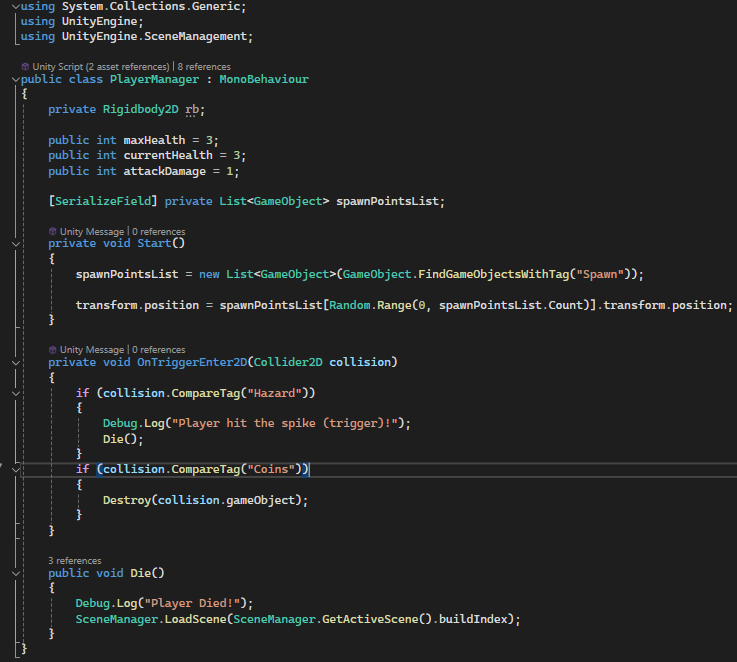
\includegraphics[width=10cm]{./Attachments/Playermanager.png}}
\caption{PlayerManager Script.}\label{fig:PlayerM}
\end{figure}
\newpage
\section{PlayerMovement }
Everything necessary for managing an extensive list of 2D character movement behaviors is entered in this class section of BasicPlayerMovement. Variables are grouped using region for organization and clarity. It comprises movement speed settings, acceleration, jump settings, wall interaction mechanics, and dash parameters. For example, variables like `moveSpeed`, `acceleration`, and `frictionAmount` control horizontal movements, while `jumpForce`, `coyoteTime`, and `fallMultiplier` fine-tune the responsiveness and feel of the jump. Similarly, wall variables ensure wall sliding and wall jumping are possible, while dash variables determine dash speed, duration, and cooldown logic.\par
It also specifies position checks for the environment, such as touching the ground or a wall, using Transform references and collision layers. Input-related variables like moveInput and jumpInput ensure the script can evaluate the player’s commands, whereas flags such as isGrounded and isDashing manage when to transition between movement states. Altogether, this block of variable declarations provides a base configuration and state management setup on which one could establish the advanced, responsive, and smooth character control of a 2D platformer.\par
 \begin{figure}[!h]
 \centering
 \fbox{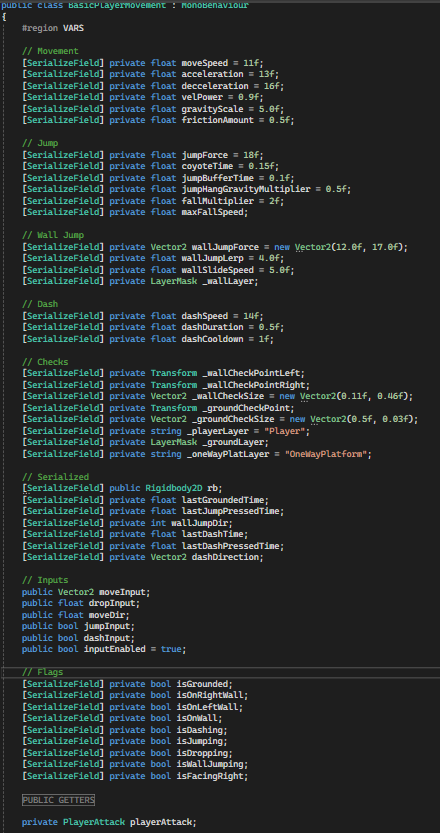
\includegraphics[width=7cm]{./Attachments/Variables_PC.png}}
\caption{BasicPlayerMovement variable section.}\label{fig:Var}
\end{figure}
\newpage
This section sets up the core behavior of the player through Unity’s lifecycle methods. In Awake(), initial values are set to prevent accidental actions on the first frame, and key components like Rigidbody2D and PlayerAttack are retrieved. The Update() method handles player input and triggers jump and dash logic each frame. Meanwhile, FixedUpdate() manages physics-related behaviors, including movement, friction, wall detection, and gravity adjustments. Together, these methods ensure the player responds smoothly to input while maintaining consistent and stable physics.\par
 \begin{figure}[!h]
 \centering
 \fbox{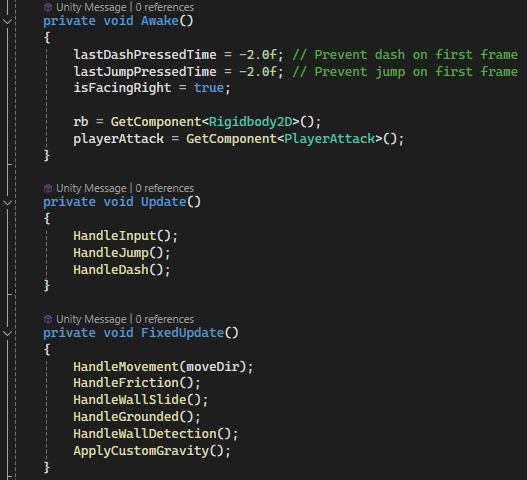
\includegraphics[width=10cm]{./Attachments/AUF.png}}
\caption{BasicPlayerMovement Initialize section.}\label{fig:AUF}
\end{figure}
The HandleInput() method captures and processes the player's real-time input. If input is enabled, it reads horizontal and vertical axis values to determine movement and drop directions. It also checks for key presses related to jumping (Space) and dashing (Left Shift). When a jump or dash input is detected, the corresponding methods (Jump() and Dash()) are called immediately, supporting features like jump buffering and responsive dashing. This function acts as the main link between the player’s physical input and the in-game movement system.\par
 \begin{figure}[!h]
 \centering
 \fbox{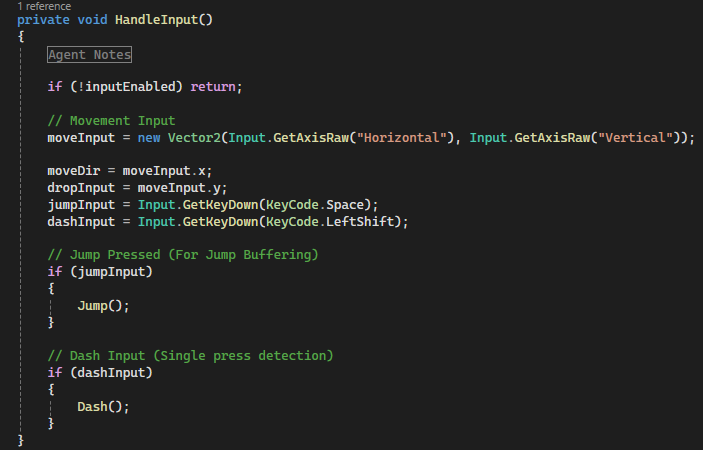
\includegraphics[width=8cm]{./Attachments/PlayerMovement_Input.png}}
\caption{BasicPlayerMovement Initialize section.}\label{fig:Input}
\end{figure}
\newpage
This method, HandleMovement(), controls horizontal movement by adjusting the player's velocity based on input direction and current state. It first exits early if the player is dashing. If the player is not attacking, the character will flip its facing direction to match movement input. It then calculates the desired speed and applies acceleration or deceleration accordingly using a smoothed velocity formula for natural movement. If the player is not wall jumping, horizontal force is applied directly; otherwise, a smoothed transition using linear interpolation (Lerp) ensures stable control during wall jumps. This function ensures responsive and fluid horizontal movement across normal and wall-jumping states.\par
 \begin{figure}[!h]
 \centering
 \fbox{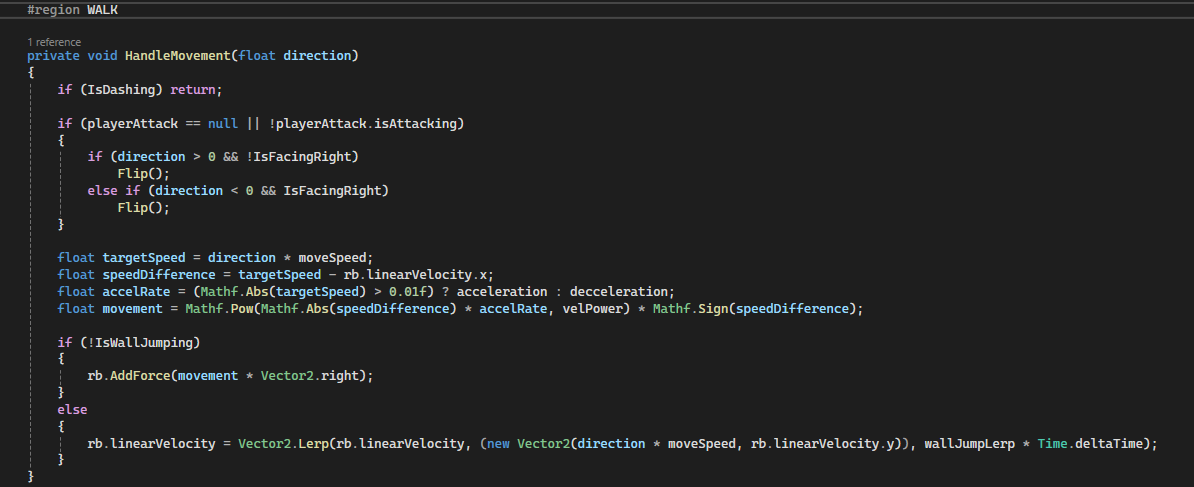
\includegraphics[width=10cm]{./Attachments/PlayerMovement_walk.png}}
\caption{BasicPlayerMovement walk section.}\label{fig:walk}
\end{figure}
This section implements both standard and wall jumping mechanics with added responsiveness through features like jump buffering and coyote time. The Jump() method logs the time when a jump is requested, or triggers a drop if the player is pressing downward. The HandleJump() method checks whether the player is allowed to jump within a short input buffer period, then prioritizes a regular jump if the player is on or near the ground, or a wall jump if clinging to a wall. Helper methods like CanJump() and CanWallJump() determine the player's eligibility for each type of jump. PerformJump() applies upward velocity for a normal jump, while PerformWallJump() calculates a directional force to push the player away from the wall. Together, these methods create a fluid and player-friendly jumping system suited for platformer gameplay.\par
 \begin{figure}[!h]
 \centering
 \fbox{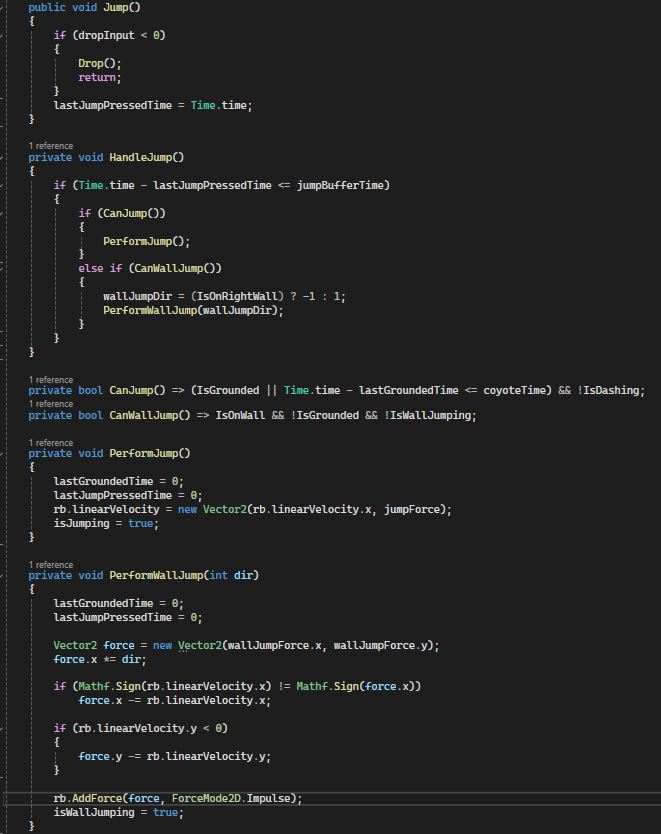
\includegraphics[width=6cm]{./Attachments/PlayerMovement_jump.png}}
\caption{BasicPlayerMovement jump section.}\label{fig:jump}
\end{figure}
\newpage
This segment manages the player's dash ability, allowing for quick bursts of horizontal movement. The Dash() method records the time a dash is requested, but only if the cooldown period has passed. HandleDash() checks if a dash can currently be performed and whether a new dash input was recently made, then triggers the PerformDash() coroutine. PerformDash() temporarily disables gravity, sets the player's velocity in the facing direction, and holds this state for a short duration. Afterward, gravity is restored, the dash ends, and the cooldown timer is reset. This system ensures dashing feels fast and responsive while maintaining balance through cooldown control.\par
 \begin{figure}[!h]
 \centering
 \fbox{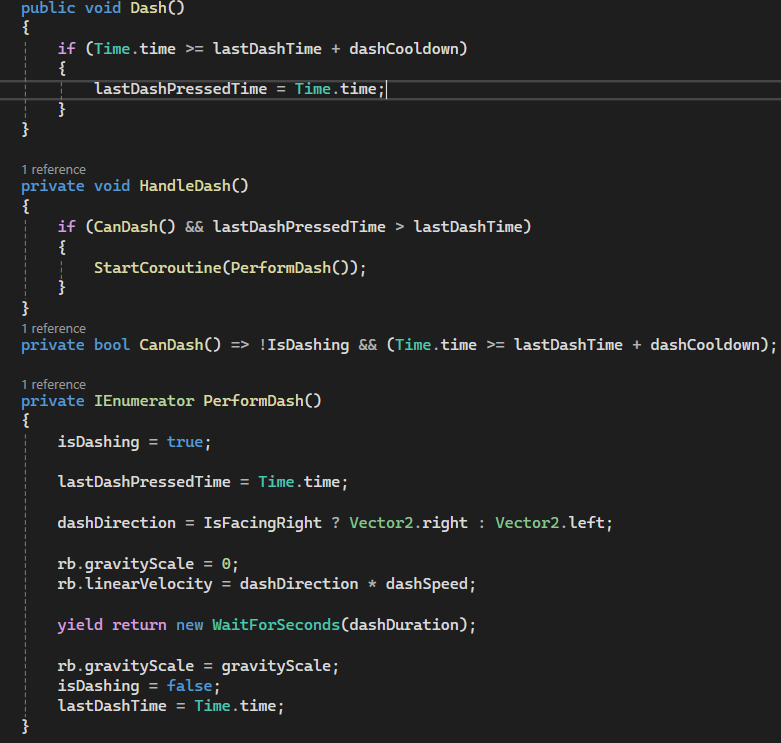
\includegraphics[width=8cm]{./Attachments/PlayerMovement_dash.png}}
\caption{BasicPlayerMovement dash section.}\label{fig:dash}
\end{figure}
The HandleWallSlide() method controls the wall sliding mechanic, which activates when the player is airborne, touching a wall, and falling downward. Under these conditions, it limits the player’s vertical velocity to a fixed negative value, defined by wallSlideSpeed. This creates a slow, controlled descent along walls, giving players more time to react and preparing them for potential wall jumps. The mechanic enhances both movement precision and gameplay fluidity in platformer environments.\par
 \begin{figure}[!h]
 \centering
 \fbox{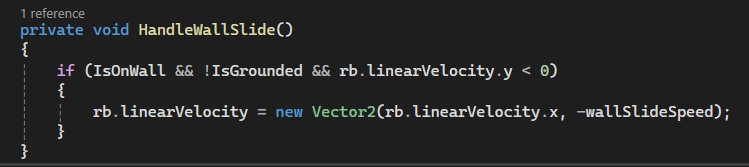
\includegraphics[width=10cm]{./Attachments/PlayerMovement_wall.png}}
\caption{BasicPlayerMovement wall slide section.}\label{fig:wall}
\end{figure}
\newpage
The Drop() method enables the player to pass through one-way platforms by temporarily disabling collisions between the player and the platform layer. This action is only triggered when the player is grounded and pressing downward. By using Physics2D.IgnoreLayerCollision, it ensures a smooth drop-through mechanic commonly found in platformers, allowing for more dynamic navigation of vertical level design. The isDropping flag can be used elsewhere in the code to manage related behaviors or animations.\par
 \begin{figure}[!h]
 \centering
 \fbox{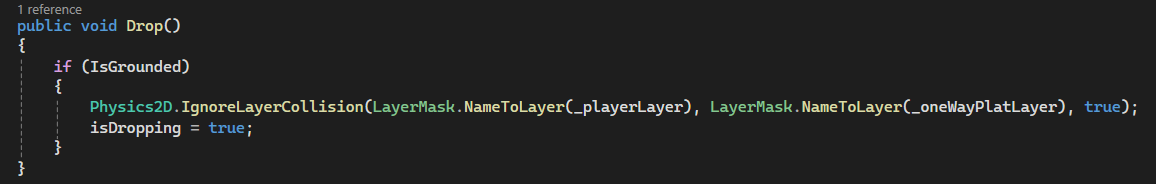
\includegraphics[width=12cm]{./Attachments/PlayerMovement_drop.png}}
\caption{BasicPlayerMovement drop section.}\label{fig:drop}
\end{figure}
These methods are responsible for detecting the player's interaction with the ground and walls, as well as managing collisions with one-way platforms. HandleGrounded() checks whether the player is currently standing on the ground using a physics overlap box and updates relevant state variables like isJumping and isWallJumping. HandleWallDetection() similarly uses overlap checks to determine if the player is touching walls on either side, which is essential for enabling wall-jumping mechanics. The OnTriggerEnter2D() method temporarily disables collisions with one-way platforms when the player is jumping upwards, allowing upward movement through them. Conversely, OnTriggerExit2D() re-enables these collisions when the player finishes dropping through a platform, ensuring consistent platform behavior.\par
 \begin{figure}[!h]
 \centering
 \fbox{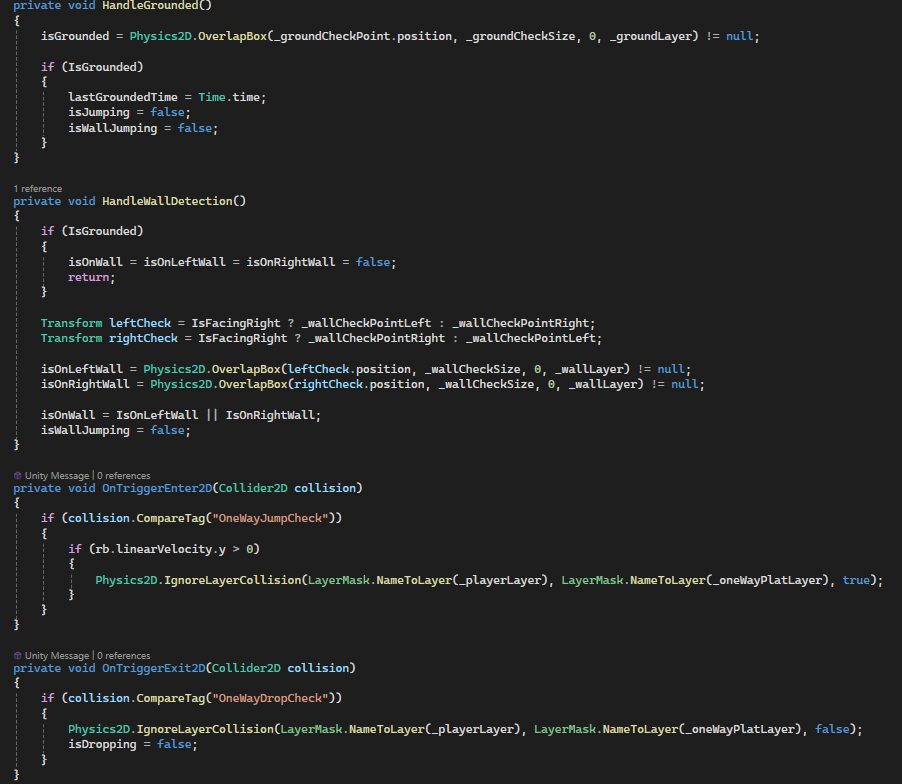
\includegraphics[width=12cm]{./Attachments/PlayerMovement_check.png}}
\caption{BasicPlayerMovement check section.}\label{fig:check}
\end{figure}
\newpage
The ApplyCustomGravity() method adjusts gravity based on the player's state to create a more natural and dynamic feel for jumping and falling. If the player is hanging after a jump (when vertical velocity is minimal), gravity is reduced to make the jump feel more controlled. Conversely, when falling, gravity is increased to make the descent faster, and a maximum fall speed is enforced to prevent excessive speed. If the player is not dashing, normal gravity is applied.The HandleFriction() method manages the player's deceleration when on the ground and not moving. It applies a frictional force to slow down the player gradually, based on the current velocity. This makes the movement feel more realistic by preventing abrupt stops and ensuring smoother transitions between movement states.\par
 \begin{figure}[!h]
 \centering
 \fbox{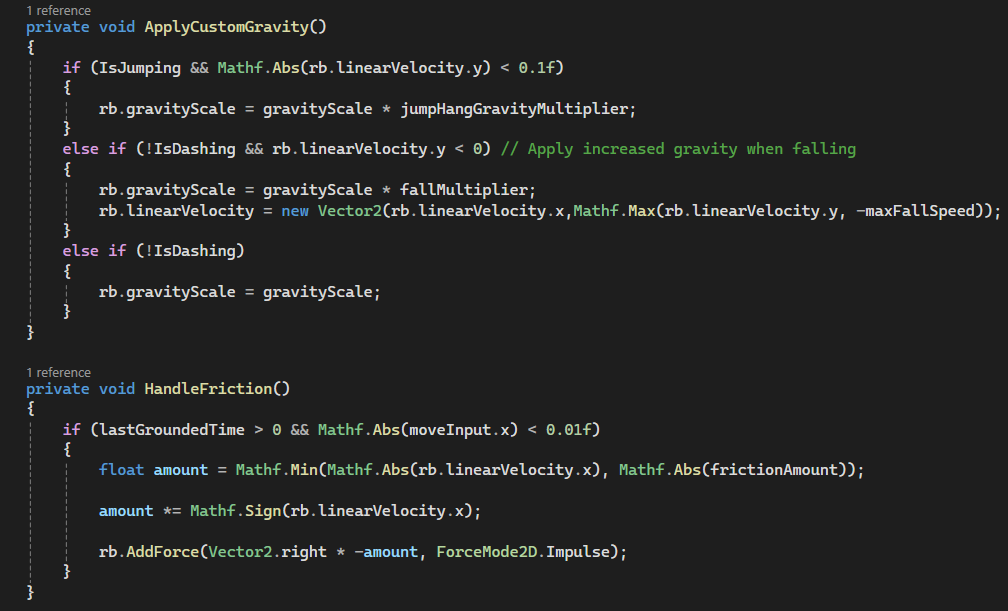
\includegraphics[width=10cm]{./Attachments/PlayerMovement_physics.png}}
\caption{BasicPlayerMovement physics section.}\label{fig:physics}
\end{figure}
The OnDrawGizmos() method is used for visual debugging in the Unity editor. It draws wireframe cubes at specific locations in the scene to represent the player's ground and wall detection areas. The green wireframe cube indicates the area where the player checks for ground, and the blue cubes represent the detection zones on either side of the player for wall detection. This helps visualize the range and orientation of the player's collision checks, making it easier to debug and fine-tune the movement and interaction mechanics during development.\par
 \begin{figure}[!h]
 \centering
 \fbox{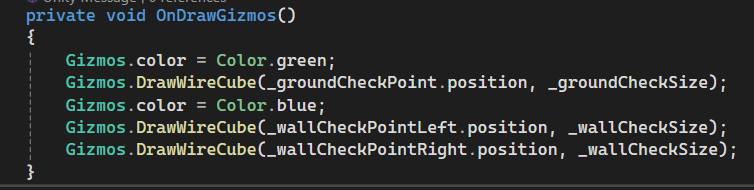
\includegraphics[width=10cm]{./Attachments/PlayerMovement_gizmos.png}}
\caption{BasicPlayerMovement gizmos section.}\label{fig:gizmos}
\end{figure}
\newpage
\section{PlayerAttack script}
The initial section of the PlayerAttack script defines the core setup for managing attack behavior in the game. It includes serialized fields such as attackCooldown to control the delay between consecutive attacks, attackDamage to determine the amount of damage dealt, and enemyLayer to specify which objects can be damaged. The script also defines attackPoint as the origin for the attack hitbox and attackCapsuleSize along with capsuleDirection to shape the area of effect. A visual effect (attackVisual) can be shown when the player attacks. The PlayerManager reference is used to fetch the player's attack damage dynamically. A public property isAttacking tracks whether an attack is in progress, while attackInput and inputEnabled manage player input. In the Awake() method, the script initializes the PlayerManager reference and sets the attackDamage accordingly. Finally, the Update() method calls HandleInput() to check for attack input\par
 \begin{figure}[!h]
 \centering
 \fbox{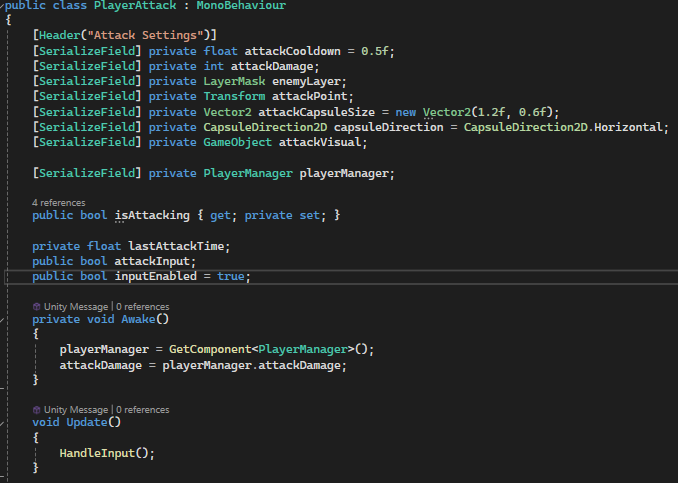
\includegraphics[width=10cm]{./Attachments/Playerattack_vai.png}}
\caption{PlayerAttack variables and initialize section.}\label{fig:vai}
\end{figure}
This section handles player input for attacking. The HandleInput() method first checks whether input is currently enabled. If it is, it listens for a left mouse button click (Input.GetMouseButtonDown(0)) and sets attackInput accordingly. If an attack input is detected, it calls the PerformAttack() method to execute the attack logic. This design ensures that the player can only initiate attacks when allowed and that attack actions are triggered explicitly by user input.\par
 \begin{figure}[!h]
 \centering
 \fbox{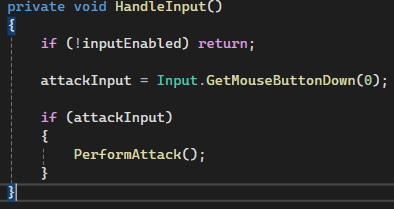
\includegraphics[width=10cm]{./Attachments/Playerattack_input.png}}
\caption{PlayerAttack input section.}\label{fig:input}
\end{figure}
\newpage
The PerformAttack() method manages the player's attack execution while respecting the cooldown period. It begins by checking whether enough time has passed since the last attack; if not, it exits early. If the cooldown has elapsed, it updates lastAttackTime, marks the player as currently attacking by setting isAttacking to true, and optionally shows a visual indicator (attackVisual) for a brief moment. It then performs a hit detection using Physics2D.OverlapCapsuleAll centered on the attackPoint, using the specified capsule size and direction to identify all enemies within range. For each detected enemy, it retrieves the EnemyActionModule component and calls its TakeDamage() method, passing in the damage value and the player’s position for knockback calculation. A debug message is logged for each successful hit.\par
 \begin{figure}[!h]
 \centering
 \fbox{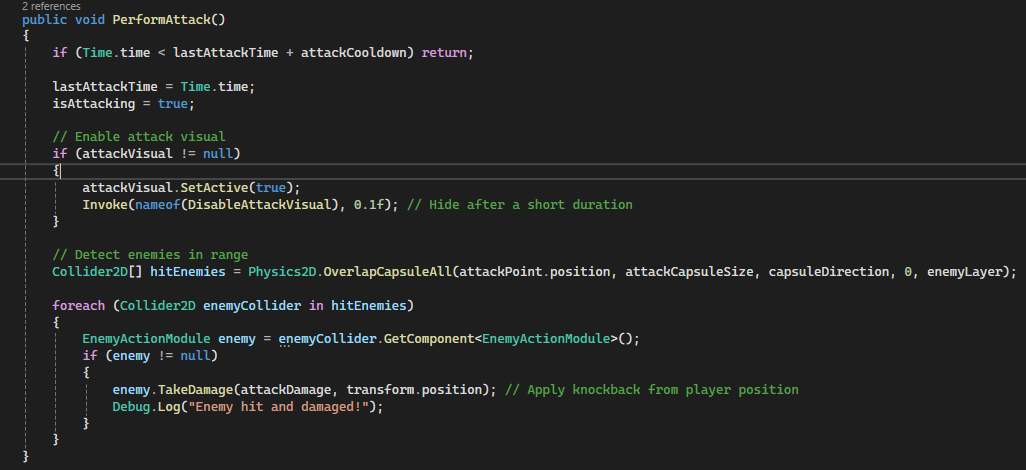
\includegraphics[width=10cm]{./Attachments/Playerattack_attack.png}}
\caption{PlayerAttack perform attack section.}\label{fig:attack}
\end{figure}
The DisableAttackVisual() method resets the attack state after a short duration. It sets isAttacking to false and disables the attackVisual GameObject if it exists, effectively ending the visual and logical representation of an attack.
 \begin{figure}[!h]
 \centering
 \fbox{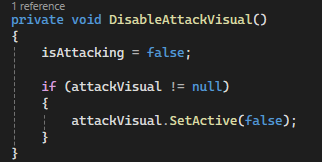
\includegraphics[width=10cm]{./Attachments/Playerattack_disable.png}}
\caption{PlayerAttack disable attack visual section.}\label{fig:disable}
\end{figure}
\newpage
The OnDrawGizmos() method visually represents the player’s attack range in the Unity editor by drawing a capsule at the attackPoint position. It calculates the start and end points of the capsule based on its direction (horizontal or vertical), draws circles at both ends to represent the capsule's curves, and connects them with lines to complete the capsule shape. This helps developers see and adjust the attack hitbox during development.
 \begin{figure}[!h]
 \centering
 \fbox{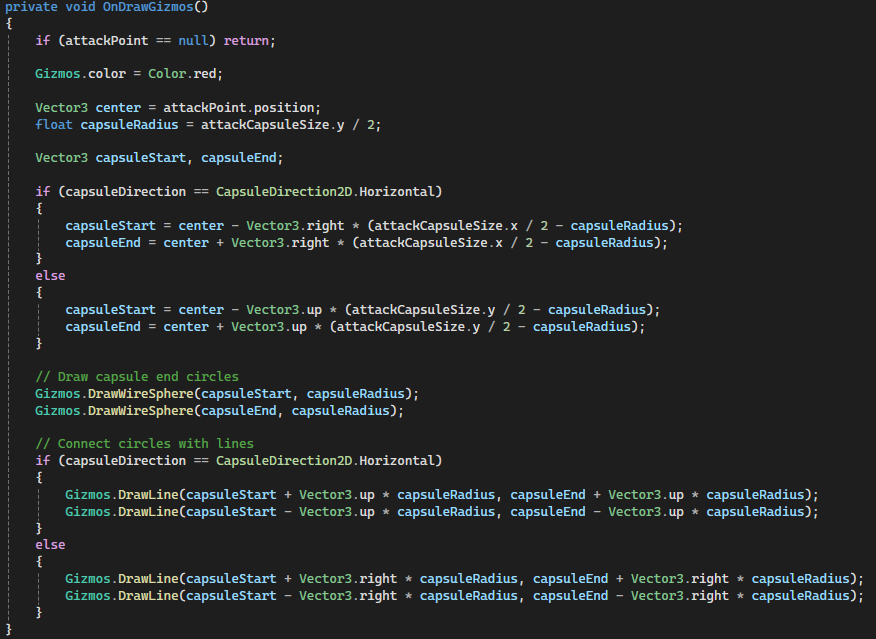
\includegraphics[width=10cm]{./Attachments/Playerattack_gizmos.png}}
\caption{PlayerAttack gizmos section.}\label{fig:attkgizmos}
\end{figure}
\section{Agent Controller}
The AgentController class inherits from Agent and integrates Unity ML-Agents with core gameplay components to enable intelligent behavior from the player character. It references two primary components via serialized fields: PlayerActionModules and PlayerManager, which likely handle character movement and overall state management, respectively. Additionally, it includes a list of spawnPointsList, a collection of potential spawn locations used to reset or relocate the agent. Internally, the class tracks the agent's last position and maintains a set called visitedAreas to record the discrete areas the agent has already explored, using Vector2Int for grid-based precision.\par
 \begin{figure}[!h]
 \centering
 \fbox{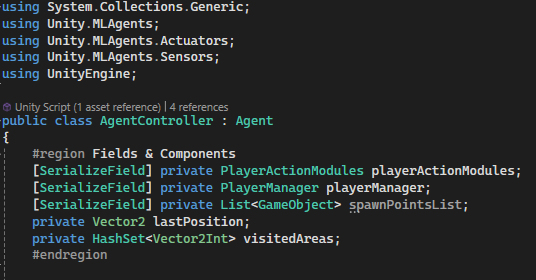
\includegraphics[width=10cm]{./Attachments/Agentcontroller_fac.png}}
\caption{AgentController fields and componenets section.}\label{fig:agentfac}
\end{figure}
\newpage
The Initialize method is an overridden function from the Agent class, responsible for setting up the agent’s initial state when the simulation begins. It first ensures that the game time is running at a normal speed by setting Time.timeScale to 1. The method then checks if the playerActionModules and playerManager are assigned; if not, it attempts to fetch these components from the same GameObject. Finally, the method populates the spawnPointsList with all GameObjects tagged as "Spawn," utilizing GameObject.FindGameObjectsWithTag("Spawn") to gather a list of spawn locations across the scene.\par
 \begin{figure}[!h]
 \centering
 \fbox{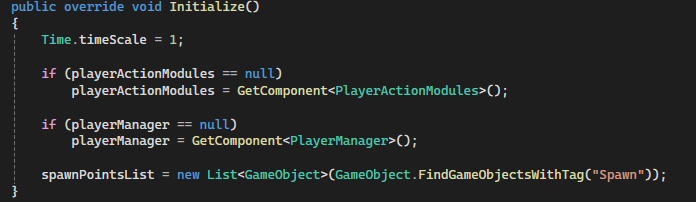
\includegraphics[width=10cm]{./Attachments/Agentcontroller_ini.png}}
\caption{AgentController Initialization section.}\label{fig:agentini}
\end{figure}
The OnEpisodeBegin method is another overridden function from the Agent class, which resets the agent’s state at the beginning of each new training episode. It first ensures that the playerActionModules is assigned, and then proceeds to disable the player’s input by calling DisablePlayerInput. The method also resets the agent's velocity and position, if the basicPlayerMovement module is available, it sets the Rigidbody2D's velocity to zero. Additionally, the method saves the agent's starting position in the lastPosition variable and initializes a new HashSet<Vector2Int> for tracking visited areas. This ensures that the agent’s movement and environment interaction are properly reset at the beginning of the episode.The DisablePlayerInput method disables input processing for both the basicPlayerMovement and playerAttack modules by setting their inputEnabled flags to false. It checks if the necessary modules are already assigned and assigns them if needed, ensuring that no player input can be processed during training.\par
 \begin{figure}[!h]
 \centering
 \fbox{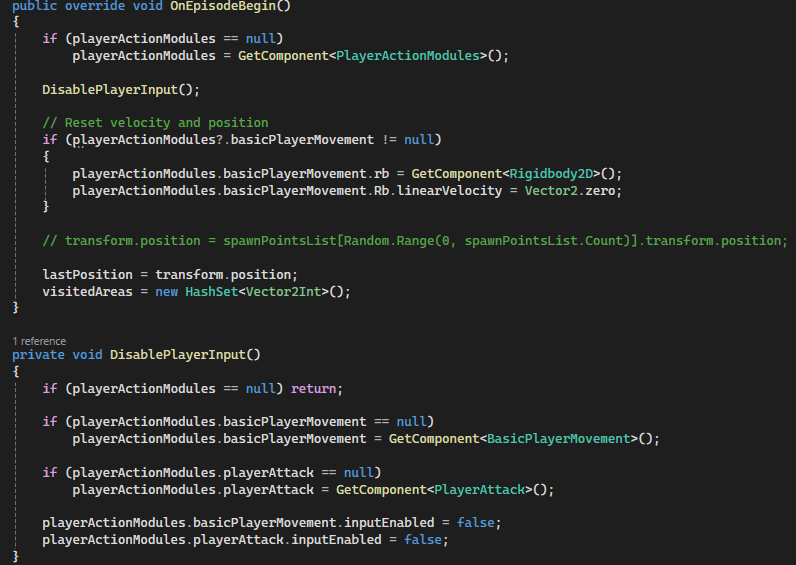
\includegraphics[width=10cm]{./Attachments/Agentcontroller_eh.png}}
\caption{AgentController Episode Handling section.}\label{fig:Epihand}
\end{figure}
\newpage
The CollectObservations method is part of Unity's ML-Agents framework and is used to collect observations from the environment that the agent will use to make decisions. In this implementation, the method gathers a series of observations regarding the player's current state, which will be passed to the reinforcement learning model to help it learn how to act in the environment.\par
First, the method checks if the basicPlayerMovement component is available. If not, it adds a fallback observation (0) and returns. If basicPlayerMovement is present, it proceeds to collect various observations. These observations include the player’s position (x and y coordinates), movement states (whether the player is grounded, jumping, facing right, dashing, dropping, on a wall, or wall-jumping), and the player’s current health.The method also collects information about the player's attack state, adding an observation that indicates whether the player is attacking. All these observations are added to the sensor, which is used by the agent to inform its decision-making during training.This method enables the reinforcement learning model to track the player's state, facilitating better decision-making based on these environmental factors.\par
 \begin{figure}[!h]
 \centering
 \fbox{\includegraphics[width=15cm]{./Attachments/Agentcontroller_observation.png}}
\caption{AgentController Observation section.}\label{fig:observe}
\end{figure}
\newpage
The OnActionReceived method in the AgentController script processes the actions received by the reinforcement learning agent. It first extracts continuous and discrete actions from the ActionBuffers parameter, interpreting the values to control various player behaviors. The continuous action, actions.ContinuousActions[0], represents the player's horizontal movement and is clamped to the range of -1f to 1f. The discrete actions correspond to jump, dash, attack, and drop, with a value of 1 indicating that the respective action should be performed. The method then delegates the appropriate actions to the playerActionModules, calling methods like Move(), Jump(), Dash(), Attack(), and Drop() based on the received input. Finally, it calls the EvaluateRewards() method to assess the agent's performance, which is crucial for the reinforcement learning model to determine the effectiveness of the actions and adjust accordingly.\par
 \begin{figure}[!h]
 \centering
 \fbox{\includegraphics[width=10cm]{./Attachments/Agentcontroller_action.png}}
\caption{AgentController Action section.}\label{fig:action}
\end{figure}
The EvaluateRewards method in the AgentController script is responsible for assigning rewards based on the agent's actions and progress within the game environment. The method first calculates the distance the agent has moved since the last update using Vector2.Distance. If the agent has moved a significant distance (greater than 0.1 units), it rewards the agent with a value proportional to the distance moved (0.05 times the distance). If the movement is negligible, it penalizes the agent with a small negative reward of -0.01. This encourages the agent to make meaningful progress rather than staying idle. The method then updates lastPosition to the current position of the agent.Next, the method checks if the agent has visited a new area. It converts the agent's position to a Vector2Int grid coordinate and checks if this position has been visited before using the visitedAreas set. If the agent has not visited the current grid position, it rewards the agent with 0.2 units and adds the grid position to the visitedAreas set to track exploration. This exploration reward encourages the agent to move to new areas and explore the environment.\par
 \begin{figure}[!h]
 \centering
 \fbox{\includegraphics[width=10cm]{./Attachments/Agentcontroller_reward.png}}
\caption{AgentController Reward section.}\label{fig:reward}
\end{figure}
\newpage
The OnTriggerEnter2D method in the AgentController script is responsible for handling the agent's interactions with different colliders during the game. When the agent collides with an object tagged with a specific label, the method uses a switch statement to determine the type of object and apply appropriate rewards or penalties. If the agent collides with an object tagged as "Coins", it rewards the agent with 1.0 unit, encouraging it to collect coins. If the agent collides with an object tagged as "Hazard", it penalizes the agent with -3.0 units and ends the current episode, indicating that a hazard results in a significant penalty and failure. If the agent encounters an "Enemy", it applies a moderate penalty of -2.0 units, discouraging contact with enemies. Lastly, if the agent reaches a "Checkpoint", it rewards the agent with a significant 5.0 unit, incentivizing progress through the game. This method helps guide the agent's behavior by providing feedback based on its interactions with key game elements.\par
 \begin{figure}[!h]
 \centering
 \fbox{\includegraphics[width=10cm]{./Attachments/Agentcontroller_collision.png}}
\caption{AgentController Collision section.}\label{fig:collision}
\end{figure}
\newpage
The Heuristic method in the AgentController script provides a manual control scheme for the agent using player input, primarily for testing and debugging in the Unity Editor. This method overrides the default Heuristic function from the ML-Agents framework and populates the actionsOut parameter with values derived from player input. It first accesses both the ContinuousActions and DiscreteActions buffers. The ContinuousActions[0] is set using Input.GetAxisRaw("Horizontal"), which captures left or right movement from keyboard inputs like the arrow keys or A/D. Then, the DiscreteActions are assigned as follows: discreteActions[0] activates when the spacebar is pressed, triggering a jump; discreteActions[1] activates when the Left Shift key is pressed, initiating a dash; discreteActions[2] triggers an attack when the left mouse button is clicked; and discreteActions[3] becomes true when the S key is held down, initiating a drop-through platform action. This method allows the developer to control and test the agent manually, bypassing the AI’s decision-making during training or demonstrations.\par
 \begin{figure}[!h]
 \centering
 \fbox{\includegraphics[width=10cm]{./Attachments/Agentcontroller_heuristic.png}}
\caption{AgentController Heuristic section.}\label{fig:heuristic}
\end{figure}
\section{Enemy Script}
The Enemy class represents a basic enemy character in the game, managing its health, invincibility state, and reactions to damage. It begins with serialized fields for maxHealth, a damageCooldown duration during which the enemy becomes invincible after being hit, and a knockbackForce that defines how strongly it is pushed upon taking damage. The currentHealth tracks the enemy's remaining life points, while isInvincible and invincibilityTimer control temporary immunity to repeated attacks. In Awake(), the enemy initializes its health and retrieves its Rigidbody2D and associated EnemyActionModule if not already set.\par
In the Update() loop, if the enemy is currently invincible, it decrements the timer until invincibility wears off. The TakeDamage() method handles damage intake, it only processes if the enemy isn't invincible. Upon being hit, the enemy reduces its health, triggers invincibility, applies knockback using the source of the attack, and checks if it should die. The ApplyKnockback() method calculates a direction vector away from the attacker and applies an impulse force to the Rigidbody2D to push the enemy back. Finally, if the enemy’s health drops to zero or below, it calls Die(), which invokes the Die() function from the action module and destroys the game object.\par
\newpage
 \begin{figure}[!h]
 \centering
 \fbox{\includegraphics[width=10cm]{./Attachments/Enemy.png}}
\caption{Enemy Scripts.}\label{fig:Enemy}
\end{figure}
\newpage
\section{Enemy Action Module}
The EnemyActionModule class acts as an intermediary that handles the enemy's interaction with the reinforcement learning agent (AgentController) and delegates core combat functionality to the associated Enemy component. In Awake(), it ensures the enemyCombat reference is assigned, typically pointing to the same game object’s Enemy component.The TakeDamage() method is called when the enemy is struck. Before delegating the damage logic to enemyCombat, it locates an AgentController in the scene and rewards the agent with +1.0 reward, reinforcing the behavior of attacking enemies. After that, it calls the TakeDamage() method of the Enemy class to apply damage, knockback, and health management.The Die() method is responsible for handling enemy death events. When invoked, it also finds the AgentController and rewards it with +5.0, incentivizing successful eliminations. Then it calls the Die() function of the Enemy class to destroy the enemy object.\par
 \begin{figure}[!h]
 \centering
 \fbox{\includegraphics[width=10cm]{./Attachments/Enemyactionmodule.png}}
\caption{Enemy Action Module Scripts.}\label{fig:Enemyactionmodule}
\end{figure}
\newpage
\section{Enemy State Machine}
This script defines the basic structure for an Enemy State Machine in Unity, which controls how an enemy behaves based on different conditions. The EnemyStateMachine class includes three defined states: Patrol, Idle, and Chase, managed by an enum called EnemyState. For patrolling, the enemy moves between a series of waypoints (patrolPoints) at a given speed. The chase behavior activates when the player enters a specified detectionRange, causing the enemy to move faster (chaseSpeed) toward the player (playerPosition). The state machine uses references to the player’s movement script (BasicPlayerMovement) and a Rigidbody2D component for motion control. A sprite GameObject is also included, likely for visual adjustments such as flipping the sprite direction.
 \begin{figure}[!h]
 \centering
 \fbox{\includegraphics[width=13cm]{./Attachments/ESM_var.png}}
\caption{Enemy State Machine variables section.}\label{fig:ESMvar}
\end{figure}
\newpage
This section of the EnemyStateMachine script sets up the enemy's runtime behavior and updates its state each frame. In the Start() method, the enemy's Rigidbody2D is initialized, and rotation is frozen to prevent unwanted spinning. It also locates the player object using FindFirstObjectByType<BasicPlayerMovement>() and assigns the player's Transform to playerPosition, which is crucial for the chase logic. A warning is logged if no patrol points are provided, helping developers catch setup issues early.
The Update() method acts as the core of the state machine. It checks the current state of the enemy (Patrol, Chase, or Idle) and executes the appropriate behavior. In Patrol, the enemy follows a set of points and also checks if the player has entered detection range. In Chase, the enemy actively pursues the player and continuously checks if the player has moved out of range to potentially return to patrolling. In the Idle state, the enemy remains stationary by setting its velocity to zero. This structure ensures that each behavior is clearly separated and triggered based on state conditions.\par
 \begin{figure}[!h]
 \centering
 \fbox{\includegraphics[width=13cm]{./Attachments/ESM_ini.png}}
\caption{Enemy State Machine initialization section.}\label{fig:ESMini}
\end{figure}
\newpage
This part of the EnemyStateMachine script defines how the enemy moves during both patrol and chase behaviors, as well as how it visually responds to direction changes.
The Patrol() method is responsible for basic waypoint navigation. The enemy moves toward the current patrol point by calculating the normalized direction vector and applying horizontal velocity using the patrol speed. When the enemy is close enough to a patrol point (within 0.2 units), it cycles to the next point using modulo arithmetic to loop through the array. The sprite is then flipped to face the movement direction using the FlipSprite() method.The ChasePlayer() method operates similarly, but instead of heading toward patrol points, the enemy calculates direction based on the player's position. It moves using a faster chaseSpeed to give the player a sense of urgency when detected. Again, the sprite is flipped to face the direction of movement for visual consistency.FlipSprite(float moveDirection) ensures the enemy's sprite visually faces the direction it's moving. It checks the horizontal movement direction and inverts the local scale’s x-axis if needed, this prevents the enemy from moonwalking or moving backward visually while chasing or patrolling.\par 
 \begin{figure}[!h]
 \centering
 \fbox{\includegraphics[width=15cm]{./Attachments/ESM_sm.png}}
\caption{Enemy State Machine State machine logic section.}\label{fig:ESMsm}
\end{figure}
\newpage
These two methods, CheckForPlayer() and CheckForPlayerOutOfRange(), control the transitions between the patrol and chase states in the EnemyStateMachine by monitoring the distance between the enemy and the player.CheckForPlayer() is used during the patrol state to detect when the player enters the enemy's detection range. If the player’s distance from the enemy is less than or equal to the defined detectionRange, the enemy enters the Chase state. Optionally, a visual indicator (like an exclamation mark or alert icon stored in the detected GameObject) is activated to signal the change in behavior.On the other hand, CheckForPlayerOutOfRange() is called during the chase state to determine when the player has moved far enough away that they are no longer considered a target. If the player moves beyond the detection range, the alert indicator is turned off and the enemy returns to the Patrol state.Together, these methods allow the enemy to dynamically switch between patrolling and actively chasing the player based on proximity, enabling more reactive and engaging AI behavior.\par
 \begin{figure}[!h]
 \centering
 \fbox{\includegraphics[width=12cm]{./Attachments/ESM_checkplayer.png}}
\caption{Enemy State Machine check player section.}\label{fig:ESMcp}
\end{figure}
This OnCollisionEnter2D method handles the interaction between the enemy and the player when a physical collision occurs.When the enemy collides with another object, the method checks if the object has the "Player" tag using CompareTag("Player"). If it does, the method attempts to retrieve the PlayerManager component from the player GameObject. If the component exists, it calls playerManager.Die(), triggering whatever logic is implemented in the player's death function, typically ending the level, restarting from a checkpoint, or triggering a death animation.This mechanic is useful for enemies that deal instant or contact-based damage, like spikes, patrolling robots, or charging creatures. It makes the enemy more threatening and reinforces the need for players to avoid direct contact.\par
 \begin{figure}[!h]
 \centering
 \fbox{\includegraphics[width=12cm]{./Attachments/ESM_collision.png}}
\caption{Enemy State Machine collision check section.}\label{fig:ESMcolli}
\end{figure}
\newpage
\section{Moving Platform script}
The MovingPlatform script defines a simple back-and-forth movement system for a platform in Unity, typically used in 2D platformer games. The platform moves smoothly between two specified points, pointA and pointB, using Vector3.MoveTowards at a given speed (moveSpeed). When the platform reaches one point, it switches its target to the other, allowing for continuous oscillation.\par
Additionally, the script handles player interactions: when the player collides with the platform (OnCollisionEnter2D), the player’s transform is parented to the platform, making the player move along with it seamlessly. This prevents the player from sliding off due to physics. At the same time, it disables Rigidbody interpolation for smoother motion syncing. Once the player leaves the platform (OnCollisionExit2D), the parent is reset to null, and interpolation is re-enabled to maintain physics consistency during free movement.\par
 \begin{figure}[!h]
 \centering
 \fbox{\includegraphics[width=12cm]{./Attachments/movingplatform.png}}
\caption{Moving Platform script.}\label{fig:movplat}
\end{figure}
\newpage



%%%%%%%%%%%%%%%%%%%%%%%%%%%%%%%%%%%%%%%%%%%%%%%%%%%%%%%%%%
%%%%%%%%%%%%%%% The 2nd appendix %%%%%%%%%%%%%%%%%%%%%%%%%%
%%%%%%%%%%%%%%%%%%%%%%%%%%%%%%%%%%%%%%%%%%%%%%%%%%%%%%%%%%












\end{document}
